\documentclass[a4paper,10pt]{article}
\usepackage[utf8]{inputenc}
\setcounter{tocdepth}{2} %Only show sections and subsections in toc.

\usepackage{longtable} %used for acro
\usepackage{acro} %list of acronyms

%!TEX root = ../main.tex
\DeclareAcronym{ui}
{
	short = {UI},
	long = {User Interface}
}

\DeclareAcronym{gui}
{
	short = {GUI},
	long = {Graphical User Interface}
}

\DeclareAcronym{gps}
{
	short = {GPS},
	long = {Global Positioning System}
}

\DeclareAcronym{zybo}
{
	short = {ZB},
	long = {Zybo Board}
}

\DeclareAcronym{can}
{
	short = {CAN},
	long = {Controller Area Network}
}

\DeclareAcronym{pdo}
{
	short = {PDO},
	long = {Process Data Object}
}

\DeclareAcronym{sdo}
{
	short = {SDO},
	long = {Service Data Object}
}

\usepackage{colortbl}
\usepackage{siunitx} %Package for SI units
\sisetup{per-mode=fraction}
\usepackage{mathdots}
\usepackage{textcomp} %Vertically centered tilde (~)
\usepackage{amsmath}
\usepackage{graphicx}
\usepackage{standalone}
\usepackage{lscape} % to rotate OD table
\usepackage{array,etoolbox}
\preto\tabular{\setcounter{magicrownumbers}{0}}
\newcounter{magicrownumbers}
\newcommand\rownumber{\stepcounter{magicrownumbers}\arabic{magicrownumbers}}

\usepackage[font={footnotesize}]{caption}
\usepackage[font={footnotesize}]{subcaption}


\newcommand{\mikkel}[1]{\todo[inline,linecolor=green!100,backgroundcolor=red!70, bordercolor=green, author = Mikkel]{#1}}
\newcommand{\martin}[1]{\todo[inline,color=blue!30, author = Martin]{#1}}
\newcommand{\thomas}[1]{\todo[inline,color=black!30, author = Thomas]{#1}}
\newcommand{\catalin}[1]{\todo[inline,color=green!100, author = CataLinux]{#1}}
%newcommand{\bb}[1]{\mathbb{#1}}

\usepackage[hidelinks]{hyperref}
%\hypersetup{
%    colorlinks = false,
%    linkbordercolor = {white},
%}


%\hypersetup{
 %   colorlinks,
 %   linkcolor={red!50!black},
 %   citecolor={blue!50!black},
 %   urlcolor={blue!80!black}
%}

\usepackage{float}
\usepackage[procnames]{listings}
\usepackage{epstopdf} %Convert EPS files to PDF format
\usepackage{pdfpages} %Utility to include pdf documents into the report, used to include datasheets in appendices.

\usepackage{tikz} 			%Utility to draw nice figures
\usetikzlibrary{shapes.geometric, arrows}
\usepackage{standalone}
\usepackage{circuitikz} 	%Utility to draw circuits in tikz

\usepackage[T1]{fontenc}	% Quotes

\usepackage{todonotes}
\usepackage{listings}
\lstset{
  tabsize=3,
  frame=l,
  language=c++,
  escapeinside={(*@}{@*)},
  basicstyle=\small,
  numbers=left,
  numberstyle=\tiny\color{gray},
  keywordstyle=\color{blue},
  commentstyle=\color{green}\ttfamily,
  stringstyle=\color{mauve},
  upquote=true
  %texcl=true 
}
\renewcommand{\lstlistingname}{Code} %Let listings have code instead of figure

\usepackage{multirow}


\usepackage{url}
\renewcommand{\UrlFont}{\large\tt}

\usepackage{chngcntr} %Change the counters of objects. Used to make figure/table and equation counting specific to the section they are in.
\counterwithin{figure}{section}
\counterwithin{equation}{section}

\setcounter{tocdepth}{2}

%Make counter of listings specific to sections
\AtBeginDocument{%
  \counterwithin*{lstlisting}{section}
  \renewcommand{\thelstlisting}{%
    \ifnum\value{subsection}=0
      \thesection.\arabic{lstlisting}%
    \else
      \ifnum\value{subsubsection}=0
        \thesection.\arabic{lstlisting}%
      \else
        \thesection.\arabic{lstlisting}%
      \fi
    \fi
  }%
}

%\usepackage[inner=2cm,outer=4cm]{geometry}

\setlength{\parindent}{0pt}

\title{Electronics - 2. Semester Project}
\author{Thomas Søndergaard Christensen, Mikkel 
Skarup Jaedicke, Martin Brøchner Andersen, Catalin Ionut Ntemkas‎}
\date{dd/mm/2016}

\begin{document}
%!TEX root = ../main.tex
\begin{titlepage}
%\newgeometry{left=3cm,right=3cm}
\begin{center}

\textsc{\LARGE University of Southern Denmark}\\[1.5cm]
\textsc{\Large MSc in Engineering - Electronics}\\
\textsc{\large 2. Semester Project}\\[0.5cm]

\vfill
\vspace{3cm}
\hrule ~\\[0.3cm]
{ \LARGE \bfseries Monitoring System for the SDU Go-Kart\\[0.4cm] }
\hrule ~\\[1.5cm]

\vfill

%\includegraphics[width=0.3\textwidth]{graphics/sdu_logo}
\vspace{7cm}
% Author and supervisor
\begin{minipage}[t]{.55\textwidth}
\begin{flushleft} \large
\textbf{Authors:}\\
230390 Martin Brøchner Andersen\\
151088 Catalin Ionut Ntemkas\\
030192 Mikkel Skaarup Jaedicke\\
100589 Thomas S. Christensen
\end{flushleft}
\end{minipage}
\begin{minipage}[t]{.44\textwidth}
\begin{flushright} \large
\textbf{Supervisor:} \\
Leon Bonde Larsen
\end{flushright}
\end{minipage}

\vspace{1cm}
Date: 19-12-2016

\vspace{1cm}

\end{center}
%\restoregeometry
\end{titlepage}
\newpage
\pagenumbering{Roman}
%!TEX root = ../main.tex
\section*{Preface}
\addcontentsline{toc}{section}{Preface}

\section*{Acknowledgment}
\addcontentsline{toc}{section}{Acknowledgment}
This project would not have been possible without the invaluable assistance and patience of our supervisor. 
A Tremendous thank you to Leon Bonde Larsen.
The process was simplified by Assistant Professor Kjeld Jensen from which the sensory equipment used in the report was supplied.
\thomas{Rewritten - needs a bit more?}
\martin{Who else should we thank? Viking Pizza?}
\mikkel{NEW URL}
\vspace{5cm}
\begin{center}
	\begin{minipage}[t]{.55\textwidth}\large
		\begin{center}
		Catalin Ionut Ntemkas\\
		\vspace{1cm}
		\hrule
		\vspace{0.5cm}
		Martin Brøchner Andersen\\
		\vspace{1cm}
		\hrule
		\vspace{0.5cm}
		Mikkel Skaarup Jaedicke\\
		\vspace{1cm}
		\hrule
		\vspace{0.5cm}
		Thomas Søndergaard Christensen
		\vspace{1cm}
		\hrule
		\end{center} 
	\end{minipage}
\end{center}

\vspace{1.2cm}
  \begin{center}
    \textsl{The report, source code, data, plotting script and simulations can be found at:}  
    \end{center}
    \vspace{-5pt}
    \begin{center}
	\renewcommand{\UrlFont}{\color{black}\normalsize\tt}
    \url{github.com/mikkeljae/SEM1PRO_ELECTRONICS}
   \end{center}
\newpage

\section*{Abstract}
\addcontentsline{toc}{section}{Abstract}
A go-kart has been supplied as a development platform for student projects at University of Southern Denmark.
In the interest of enabling more complex projects, a unified data collection system is necessary.
This is developed throughout this report. 
An analysis is done to determine the requirements of such a system.
It was found that a two-part network is suitable for this application.
The two parts are a CAN network and an ad-hoc WiFi network.
A custom protocol for use on CAN, GoCAN, is developed.
GoCAN supports up to 16 sensors from which data can be monitored on a remote monitoring station using the WiFi connection.
The system was only partially implemented since a connection between the CAN network and Linux was not achieved.
\thomas{Rewritten}
\newpage
\tableofcontents
\newpage
\listoftodos
\listoftables
\addcontentsline{toc}{section}{Acronyms}
\printacronyms
\clearpage
\newpage
\pagenumbering{arabic}
\part{Preface}
%!TEX root = ../main.tex
\section{Introduction} % (fold)
\label{sec:introduction}
Something here....
% section introduction (end)
\newpage
%!TEX root = ../main.tex
\section{System Description}
\label{sec:system_description}
This project is aimed at developing a backbone for data collection on the SDU go-kart.
As mentioned, the go-kart is intended as a development platform to be used by students on the master's programme in electronics on SDU.
Some projects may implement new sensory equipment while others may work on improving the inverter.
Common for all of them is that they require access to the data that their system is producing.
Providing a unified structure for gathering data from the go-kart will greatly ease the development on the platform, especially across different projects with different developers.
A system will be developed which provides a simple method for accessing data wirelessly on the go-kart while driving.
Live access of parameters while driving, realistically, requires some form of wireless communication between a monitoring system and the go-kart, see figure \ref{fig:simple}.

\begin{figure}[h]
 	\centering
    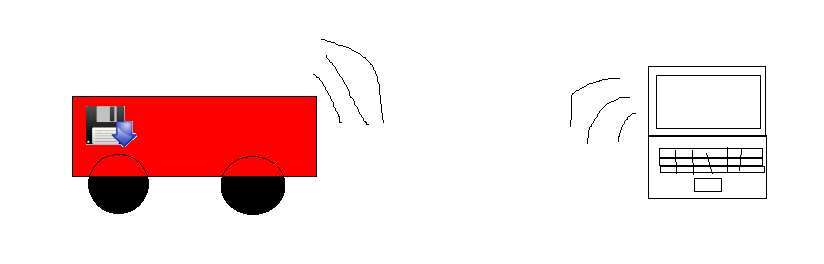
\includegraphics[width=0.6\textwidth]{graphics/go_kart_network_simple}
    \caption{SDU go-kart transferring data to a stationary computer wirelessly.}
    \label{fig:simple}
\end{figure}

While the system should be able to provide a live feed of the data being collected on the system, it should also log all data during a drive, with the possibility of transferring it later.
This will enable the user to do more advanced data analysis on the dataset than what can be achieved by monitoring the data.
In some cases, certain parameters may be irrelevant to the test being performed.
Transmitting these parameters should be avoidable by providing the possibility to start and stop data collection from specific data producers.

\begin{figure}[h]
 	\centering
    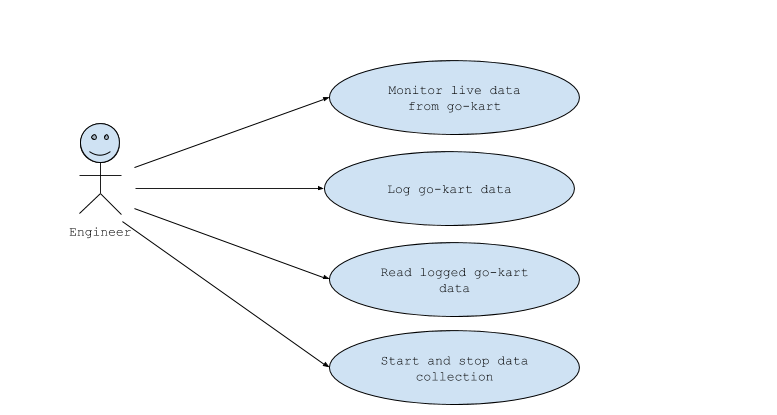
\includegraphics[width=1\textwidth]{graphics/use_cases}
    \caption{Use case diagram for the system.}
    \label{fig:usecases}
\end{figure}

As the goal of this system is to ease development on the go-kart, it should not only ease data collection, but also allow for simple addition of new sensors or other equipment.
Different projects may also have different requirements in terms of the presentation of data.
For this reason it should be possible to add a custom (G)UI of the projects design.
These requirements introduces a distinction between the actors expected to work with the system, the user and the developer.
The user will use the system to extract data from the system.
The developer will work on integrating new data producers into the system.
A use case narrative for each of the use cases is shown in appendix \ref{app:usecase}.
\newpage
\part{Analysis}
%!TEX root = ../main.tex
\section{System Analysis} % (fold)
\label{sec:system_analysis}
A thorough system analysis is needed in order to design an embedded system that meets the needs expressed by the use cases. 
This section will present the analysis of the complete embedded system, through the following topics:

\begin{itemize}
\item Parameters of interest. The use cases do not describe what parameters should be monitored meaning that it should be investigated which are relevant to monitor.
\item Hardware for monitoring parameters. It should be analysed what hardware is necessary in order to measure the parameters found to be relevant. 
\item Amount and frequency of data????. Something clever about this. Martins sections should be used for it.
\item Data collection. It should be analysed how data is collected on the go-kart.
\item Micro-controller. It should be analysed what micro-controller should be used on the go-kart.
\item Wireless network. It should be analysed how data is transferred from the go-kart 	to the stationary computer.
\item Local storage. There needs to local storage on the go-kart and it needs to be analysed what kind this should be and how it should be implemented.
\item Software on stationary computer. It should be be analysed how the software on stationary should prensent the transferred data to the user in an UI.
\end{itemize}

\subsection{Parameters of Interest}
\label{sec:parameters}
In developing new hardware or evaluating current hardware, it is necessary to be able to monitor a range of parameters.
This section will investigate what parameters need to be logged in order to provide a useful and complete logging of the behavior of the go-kart.
The parameters in question fall into three categories; Physical parameters, electrical parameters and mechanical parameters.
These will be dealt with in turn in the following sections
\paragraph*{Physical Parameters}
This category comprises all information about the motion of the go-kart.
\begin{itemize}
	\item \textbf{Position, Absolute:} Providing a means to record the absolute position of the go-kart is a useful feature in certain fields.
	Especially any form of localisation and path finding will be able to put this information to use.
	The absolute position of the go-kart can be recorded using a GPS module or possibly by using a known starting coordinate and information about the relative movement of the go-kart.
	\item \textbf{Position, Relative:} The relative position of the kart can be, as just mentioned, used to infer the absolute position of the go-kart.
	Additionally it can provide a means to analyze a drivers performance on track the or detect drift while cornoring.
	The relative position includes both translational, as well as rotational information.
	This information can be gathered using an inertial measurement unit (IMU).
	An IMU is a compound device, comprising of an accelerometer and a gyroscope and, in some cases, a magnetometer.
	\item \textbf{Velocity:} The velocity of the go-kart is key in optimising lap-times, clearly, it is desirable to monitor this parameter.
	It can be extracted by reading the motor encoders.
	However, the driving wheels are prone to slippage when cornoring, this would give an inaccurate reading of the actual velocity of the go-kart.
	Instead, a simple encoder can be mounted on either one, or both of the front wheels as these are freerunning and independent.
	Once the rotational speed of the axle is known, the velocity of the go-kart can be infered using the tyre diameter.
	\item \textbf{Acceleration:} It may be of interest to monitor the forces exerted on the go-kart, or, its acceleration, as it drives on the track.
	This information is already provided by the accelerometer in the IMU mentioned above and as such provides no additional complication.
\end{itemize}
Three sensors are mentioned in this section.
A GPS, an IMU and an encoder.
In order to limit the scope of the project only the GPS and the IMU will be implemented.
\paragraph*{Electrical Parameters}
This category comprises all information about the electrical aspects of the go-kart.
\begin{itemize}
	\item \textbf{Motor Currents:} Providing a means of monitoring the currents flowing through the motor allows the user to calculate the torque exerted by the motor as well as the current power draw of the motor.
	Knowing the currents could also prove an invaluable debugging tool when developing a new inverter for the go-kart.
	\item \textbf{Throttle Position:} The throttle on the go-kart is connected to a potentiometer.
	Measuring the voltage output of this potentiometer provides a simple way of monitoring the position of the throttle.
	\item \textbf{Desired Currents:} Based on the current throttle position a set of desired currents are calculated.
	Monitoring these allows spotting any discrepancies between the desired and the actual currents.
	\item \textbf{Duty Cycles:}
	\todo[inline]{Mikkel: What do you mean?}
	\item \textbf{Battery Voltage:} As the go-kart is electrical, naturally, it has a battery.
	Monitoring the current battery status could give the user an indication of how much driving time is left, or how long until the batteries are recharged afterwards.
	\item \textbf{Motor Angle:} Knowing the angle of the motor at all times gives a means of more accurately calculate the currents at specific times.
	Additionally, it can be used in Clarke-Parke transformations, again, providing information in debugging an inverter in development.
\end{itemize}
These parameters are all available from the sevcon gen4 motor controller mounted on the go-kart.
This controller has a CANopen interface from which this data can be extracted.
Any users who wish to add their own inverter will simply need to obey the API stated by the sevcon gen4 CANopen interface in order to correctly log the data.
\paragraph*{Mechanical Information}
This category comprises all information about the mechanical aspects of the go-kart.
\begin{itemize}
	\item \textbf{Steering Wheel Angle:} Monitoring the angle of the steering wheel allows analysing the performance of the driver.
	In addition it opens up for the possibility of mechanical control of the go-kart.
	Similarly to monitoring the velocity, the steering wheel angle can be monitored by adding an encoder to the steering column.
	\item \textbf{Braking Pedal Position:} The braking system on the go-kart is similar to that of an ordinary car.
	The braking disc is mounted on the driving axle and the braking calibers connected to the brake pedal by a series of oil-filled hoses.
	Monitoring its actuation allows analysing the performance of the driver and as mentioned above, may potentially allow for mechanical control of the go-kart
\end{itemize}
As both of these parameters would require mechanical changes to the go-kart, they are beyond the scope of this project and as such will not be implemented.
\subsubsection*{Conclusion}
In this section a multitude of different parameters have been discussed.
Most of them can be logged using just three components; a Sevcon Gen4 motor controller, an IMU and a GPS.
These are the three components from which data logging will be implemented throughout this project.
This provides a solid platform to prove the concept and additional sensory equipment can be added at a later date, should it be required.


























\subsection{Hardware for Monitoring Parameters}
\label{sec:hardware_for_par}
In section \ref{sec:parameters} an overview of the different parameters that may be of interest for logging is given.
It was concluded that three components would suffice as a proof of concept; the Sevcon Gen4 motor controller, an IMU and a GPS.
This section will explore in more detail what requirements and communication schemes exists for each of the components.

\subsubsection*{Sevcon Gen4 Motor Controller}
\label{sec:interfacin_with_sevcon}

The Sevcon Gen4 motor driver is a general purpose AC motor driver. 
This means, it can be used for both asynchronous and synchronous motors of a wide range of sizes.
The controller can then be set up for the particular motor and peripherals, and run without interfacing to another computer.
However, it is also possible to read data from it while running, and in some cases set values.
It is therefore possible to use this to access the electrical parameters. \\
\todo[inline]{Mikkel: Martin add something here about CANOPEN?}


\subsubsection*{Inertial Measurement Unit (IMU)}
\label{sec:imu}
IMU's, generally, exist in two versions.
A 6D and a 9D version.
Both include an accelerometer and a gyroscope.
In addition to these the 9D IMU includes a magnetometer, enabling measurement of absolute direction, as opposed to the relative measurement of direction granted by the magnetometer.
The requirement in terms of each of these parts is given as:
\begin{itemize}
	\item \textbf{Accelerometer [\si{\metre\per\second^2}]:} As the name implies, the accelerometer measures accelerations.
	That is, when the component changes speed or direction the force exerted on the accelerometer is measured.
	Professional drivers using professional grade go karts driving upwards of 250 \si{\kilo\metre\per\hour} can reach up to 2-3 g's of force exerted on them.
	The go kart available in this project has a theoretical maximum speed of 50 \si{\kilo\metre\per\hour}.
	Clearly, the forces exerted on this platform will be lower, however, a minimum requirement of $\pm$ 3g will be set for the accelerometer in the IMU.
	\item \textbf{Gyroscope [\si{\degree\per\second}]:} 
\end{itemize}
\thomas{Short conversation about the vectornav and why it fulfills the requirements.}

\subsubsection*{Global Positioning System (GPS)}
\todo[inline]{Mikkel: Something here?}


\subsubsection*{Conclusion}
\todo[inline]{Table with chosen sensors and their interfaces}


\subsection{Data Rate}
This section will explore the amount of data that can be expected from a sensor connected to the system.
In section~\label{sec:parameters}, a number of different parameters are presented which may be of interest to monitor.
Many of these parameters pose different requirements in terms of the desired sample rate as well as the size of each sample.
A temperature sensor, for instance, does not require nearly the same sampling frequency as an accelerometer.
Due to these differences, clearly, the data rate expected from one sensor may differ wildly from another.
In order to provide a safe estimate, the expected data rate is calculated using a "worst-case" sensor.
That is, the type of sensor which set the highest requirements in terms of sampling frequency as well as data size.
The IMU chosen for this project, see section~\ref{sec:imu}, is a 10-axis sensor.
It provides data at a rate up to 300\si{\hertz} at 32 bit floating point precision.
This would result in a data rate of:

$$300\cdot32\cdot10=96\,\text{Kb/s}$$

As previously mentioned, this is the assumed worst case for the system.
As such there may be only a few sensors providing data at this rate.
Most other sensors will provide only limited data in relation to the IMU, either due to a much lower sampling frequency or an overall smaller data size.
A GPS generally provides an update only at a few \si{\hertz} and an encoder, while it may have a reasonably high sampling rate, it is most likely not close to 32 bit resolution.
\\~\\
Assuming five sensors running at the assumed worst-case rate and ten running at half that rate, the resulting data rate will be 960 Kb/s or approximately 1 Mb/s.

% \subsection{Data Logging}
% \todo[inline]{Mikkel: Should maybe change name?}
% A feature will be data logging. 
% Any data could be put into the log, although some signals can be logged at significantly higher rates than others
% If all data is recorded at the fastest rate, this could present a storage problem.
% This challenge will be analyzed here.

% \subsubsection{Sample Rate}
% Datalogging should be useful for working with an inverter as was the case on the first semester.
% Likely it would be interesting to log the phase-current to the motor at high enough rate to accurately depict their sinusoidal short term average.
% The ripple current or voltage at the motor terminals should be measured in the lab, as this requires a high sample rate, and more control than offered on the test track.
% This data logging would be useful for recording current in the motor as the go kart is driving.
% Additionally it would be relevant to record the encoder output, and possibly the DC voltage at the input of the inverter and the duty for each phase.
% Only the currents are bound to change rapidly, and as such they determine the minimum acceptable sample rate.
% By looking at the maximum frequency of the motor and the most extreme rate of change permissible by the armature inductance, it is possible to set a sample rate for the log file.\\

% According to the manufacturer of the motor, the maximum rotational velocity is 5000 RPM.
% With four pole pairs, this comes to a maximum sinusoidal frequency of 333 Hz. 
% It is not necessary to record at a rate significantly larger than the Nyquist limit in order to adequately record the sinusoidal.
% Simulations show, that by using Clark-Park transformation, interpolation and then the inverse Clarke-Park transformation, there is nearly no difference between a low sample rate of $1\si{\kilo\hertz}$, and a higher sample rate of $3.3\si{\kilo\hertz}$, as shown below.

% \begin{figure}
% 	\centering
% 	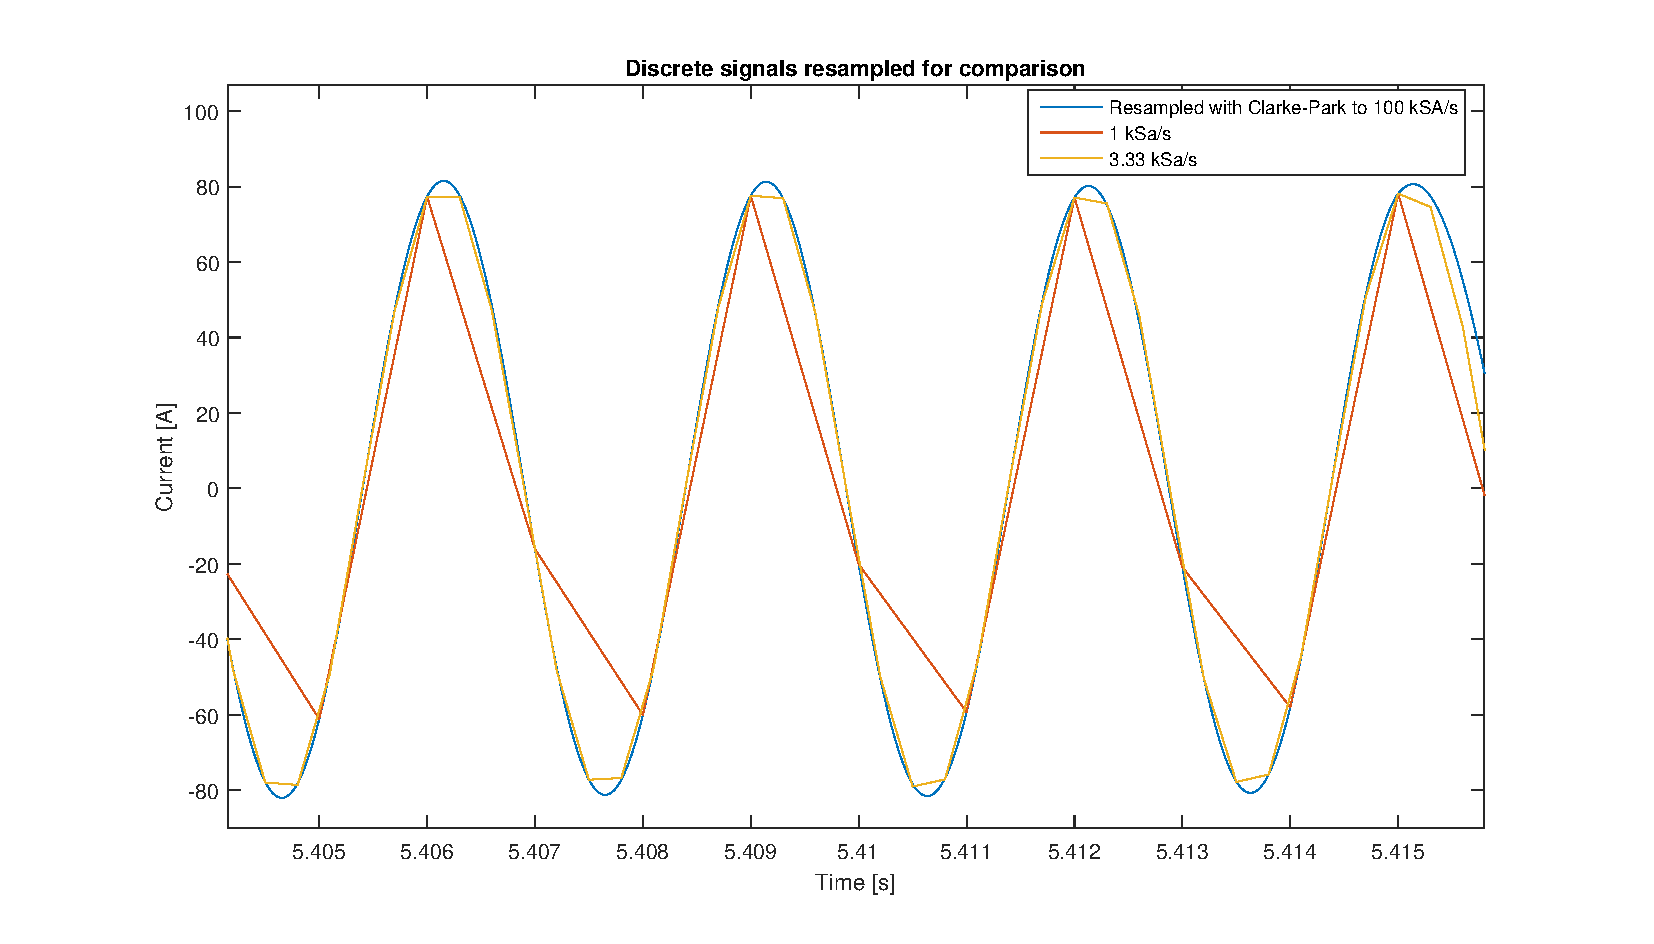
\includegraphics[width = 0.9\linewidth]{graphics/Clarke-park_resampled}	
% 	\caption{Comparison of data recorded at 1 kSa/s and 3.33 kSa/s, against 100 kSa/s resampled using Clarke-Park}
% 	\label{fig:Clarke-park_resampled}
% \end{figure}

% The resampled data from the 1 kSa/s and 3.3 kSa/s (orange and purple respectively on figure\ref{fig:Clarke-park_resampled}) are almost identical.
% However, there is a small visible difference around the time 5.527 s, likely due to the limited precision of the encoder.
% This also doesn't take into account any disturbance or noise, which could make it hard to reconstruct the signals with lower sample rates.\\

% Additionally, the Matlab function, resample, produces nicely filtered vectors with smaller time steps, so it is possible to use a low sample rate for time invariant signals.\\
% Another way to look at this is to calculate the maximum change in current from one sample to another.
% This is determined by the inductance of the motor, which is $600 \si{\micro \henry}$ \todo[inline]{when one half bridge is high, and the two others are low, it's one armature inductance of 400 uH in series with two parallel armature inductances}, and the maximum voltage across it, which is $V_{BAT}=52.8 \si{\volt}$. 
% At a sample rate of 3.33 kSa/s, this results in a theoretical maximum step of $264\si{\ampere}$.
% A sample rate lower than this, would make it hard to properly record such sudden steps.

% \subsubsection{Data Type}
% When the sample rate is known, it is possible to get an estimate of how much storage space would be needed. 
% It would be easiest, and most useful, to record using simple comma separated files, but these tend to take up more space than necessary.
% The analog input to the Zybo are 12 bit, which means, that full precision of these would be possible with 4 digits, and often a decimal point and potentially a negative sign.
% Including the horizontal separator, this comes to 6.5 bytes per point.\\

% An example of recording could include time, two currents, a voltage and the encoder output, as displayed below
% \begin{lstlisting}
% Time	Ia	Ib	V	Encoder
% 1.0000	052.3	-278.1	52.56	16
% 1.0003	057.7	-280.4	52.54	17
% \end{lstlisting}
% That brings each line length to 32 bytes (8 bytes for time, 5.5 for the three analog, 3 bytes for encoder, 5 for separators).
% At a sample rate of 3.33 kSa/s, this comes to 6.1MB per minute. 
% With the current SD cards having 4 GB of free un-partitioned space, this gives up to 11 hours of recording time.\\

% Alternately, it is possible to invent a file structure, that allows several arrays of with different data types.
% By storing numbers in binary files instead of text, it is possible to reduce the space requirements to a third (2 bytes per analog, 4 bytes per timestamp (allowing up to 49 days of ms), and 1 byte for encoder).
% This however will reduce the readability greatly, and include the workload, as one will need to write code both for encoding and decoding the file. \\

% Since this is out of the scope of this project, and the sample rate isn't larger than it is, logging in standard ASCII will suffice.
% Likely, different sample rates will be recorded to different log files









\subsection{Data Collection}
\label{sec:data_collection}
As described earlier there needs to be several sensors on the system in order to measure relevant parameters.
It should also be possible to add sensors at a later time by other developers. 
One micro-controller could be used for all sensors, but it would not be feasible when the numbers of sensors grow. 
The micro-controller would not have enough I/O peripherals to accommodate a lot of sensors. 
It might also not have the needed computational power. 
\\
Therefore a network needs to be realized. Each node in the network being a micro-controller and one or more sensors.
All sensor data needs to be collected by a node that transfers it wirelessly to the stationary computer.
This node will also need to log data as this eases the task of transferring log data to the stationary computer.
This node will be referred to as the wifi node.

\subsubsection{Network Topology}

There are various network topologies that can be used to setup the required node network for this project.
These include the ring-, bus-, mesh-, star- and tree-network topology. 
Before choosing a topology, a brief description of the purpose and functionality of the network as well as an overview of their advantages and disadvantages are needed. 

\paragraph{Purpose of the Network}~\\
\todo{Add the abbreviation ov = on-vehicle somewhere somehow}
The purpose of this network is to accommodate multiple nodes, such as sensors sub-networks and in general data-producers.
These nodes need to be able to transfer their data and receive massages from the wifi node.

The reasons for this is, that the use cases specify that sensor data should be transferred wirelssly and it needs to be possibly to start and stop specific nodes.
\\\\
The communication between the various nodes and the wifi node does not require a central hub.
Furthermore, in the case that one node fails, the network as a whole should still be operative.
Since it is a multi-node network and it may require more nodes in the future, scalability is also required.

\paragraph{Different Topologies}~\\
\todo[inline]{Thomas: This section needs to be cleaned of any statements such as "this is the simplest and cheapest...". They are broad conclusions that we have no merrits on saying}
\begin{itemize}
\item \textbf{Bus:} This is the simplest and cheapest topology.
All nodes communicate through a central bus and it is scalable with the addition of extra nodes on the two ends of the cable.
The central bus introduces the risk of complete network failure in case of the bus failure and the decrease in performance in case of many nodes or heavy traffic.
\item \textbf{Ring:} All the nodes in this type of network form a ring, where each node is connected to its two neighbors.
It has the advantages of the bus network as well and it shows better performance, even under heavy load.
A centralized control is not required for this type and in case of a node failure, the ring breaks and it can continue to function as a bus network.
It is scalable, but to a less extent than the bus.
\item \textbf{Mesh:} In this type, each node has direct connections to each other node present in the network.
That provides speed and reliability in case of node failures, but requires more hardware and processing power to manage the connections.
It is very robust but scalability is certainly not one of its features.
\item \textbf{Star:} The star topology is a centralized type of networking.
All nodes are connected to a central hub, handling all the communication between them.
It is fast, easy to implement and offers great reliability in case of node failures.
The major disadvantage is that if the hub fails, the entire network fails.
It can be scalable to a certain point, since the hub can be upgraded to handle more connections.
\item \textbf{Tree:} The last type, the tree is an extension of the bus and the star topologies combined.
It can be easily scalable, but that adds extra difficulty in its maintenance.
It also requires a lot of connections and in case the top (root) node fails, then all the network is down as well.
\item \textbf{Hybrid:} The last type is the hybrid one, where depending on the needs and purpose of the network, two or more topologies can be combined to achieve the best balance between their advantages and disadvantages.
\end{itemize}

\paragraph{Suitable Topology}~\\
For the systems networking purpose, the mesh type is not suitable, since it adds extra hardware requirements such as processing power and many redundant connections.
A node may be a simple sensor with a small micro-controller and hence, connecting it to such a network is not feasible.
%In our system, a small embedded board computer will be the ov-computer which requires to maintain its connection with the network even in case of failures and also possibly the central hub in centralized topologies that such as the star and the tree.
The star network requires a lot of connections which normally are not present at standard micro-controllers.
%Thus, these two topologies are not suited, since in case of its failure, the whole network fails.
Thus, the mesh and star networks are not suited for this system
Scalability is also a requirement for the future connection of nodes.
Although the majority of the types provide a level of scalability, the addition of extra nodes always decrease the overall performance of any network.
Hence, a topology that balances the decrease in performance against the network's expansion is best suited for the project.\\\\
The approach that fits the requirements is implementing a bus network, where each node may be a subnetwork of a different type depending on the needs, making it into a hybrid network having a bus topology as its basis.
This type provides a good balance of reliability, scalability, hardware requirements and communication speed in comparison to the others.

\subsubsection{Networking technology}

\paragraph{Existing Technologies}~\\
Different networking technologies exist in use today, such as Ethernet, CANbus, CANopen and Powerlink, among others.
CANbus is widely used in the automotive industry with data rates up to 1Mbit/s for small networks lengths, but the classic Ethernet and Powerlink support data rates of at least 10Mbit/s.
Furthermore, Powerlink is suitable for transmission of time-critical data and timing-synchronization of the nodes and CANopen networks are very robust and reliable.
\paragraph{Choosing a Technology}~\\
\todo[inline]{Mikkel: Remove were..}
The two choices that were considered for the scope of this project were Powerlink and CANopen.
The first one can be implemented using openPowerlink at a software level and utilizing PmodNIC100 modules provided by the university.
On the other hand, CANopen can be implemented using CANopenSocket\footnote{https://github.com/CANopenNode/CANopenSocket}, an open source git project built on CANopenNode.
This library is easily implemented in Linux and can use various hardware, one of them being a USB to CAN interface board named USBtin\footnote{http://www.fischl.de/usbtin/}.
Another available module to use is the CANbus.
Since CANbus is a technology widely used in the automotive industry, it is chosen for this system.



\subsection{CAN-bus}
The CAN (Controller Area Network) protocol was originally developed in the 1980's by Bosch.
It is a multi-master network, where each node connects to a common bus.
All nodes are able to broadcast data to all other nodes.
The CAN protocol includes an overhead of 47 bit per message.
The data sent in a message can vary in size from 0 to 8 bytes.
This is described in detail in section~\ref{sub:CanMessageFrame}.
The bus offers 1 Mbit/s on a bus of up to 40 \si{\metre} of length.

\begin{figure}[h!]
	\centering
	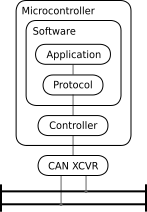
\includegraphics{graphics/canbus_setup}
	\caption{CAN node architecture}
	\label{fig:canbus_setup}
\end{figure}

Some hardware is necessary in order to properly realise a CAN network.
The structure of each node can be seen on figure~\ref{fig:canbus_setup}.
The following paragraphs explain the physical parts of this structure as well as the requirements of the protocol.

\todo[inline]{Thomas: My understanding of our protocol is that we are just interpreting the CAN messages in a different way. Do we actually need a detailed explanation of the actual CAN protocol?}
\todo[inline]{Thomas: Split this entire section into paragraphs, one for each (meaningful) box in figure~\ref{fig:canbus_setup}}

\paragraph*{The CAN Bus}~\\
The bus is shown on the bottom of figure~\ref{fig:canbus_setup}.
It is a differential signal bus.
This means that the value on the bus is determined by the difference of the two wires, rather than the absolute value of either signal.
The bus has to be made of twisted pair wires with a characteristic impedance of $\si{120 \ohm}$ and terminated at each end with a $\si{120 \ohm}$ resistor.
That means, that if the bus is broken at any point, no communication will work, even if two nodes are still connected.
Alternatively, it is possible to terminate each node, but this greatly reduces transmission speed.\\
\todo[inline]{Mikkel: Not sure I understand it.}
\paragraph*{The CAN Transceiver (XCVR)}~\\
The transceivers translate a Tx voltage signal to the differential CAN signal, and simultaneously translates the bus signal to Rx voltage signal. 
For this reason, it is not possible to implement this in most if not all microprocessors.
Because the CAN bus is differential, a transceiver would be able to read the signal it's putting out itself, but they do not transmit these to the Rx pin of the controller.
Other than this blocking of its own signal, it will translate whatever the controller puts out with.
CAN transceivers are reasonably simple in design and while they can be procured, it was decided to create a custom transceiver.
\todo[inline]{Mikkel: Above section is confusing for me.}
\todo[inline]{Thomas: And me too, The actual role of the xcvr is not clear from the text.}
\todo[inline]{Thomas: What analysis resultet in us deciding to build our own? Is this the right place for this decision?}

\paragraph*{The CAN Controller}~\\
This element can be standalone hardware, but it is in many cases built into the micro-controller.
The major advantage of having the controller built into the micro-controller is that it would not otherwise require another protocol to communicate between the microprocessor and controller.
\todo[inline]{Thomas: You mean that you would have to communicate with the controller through I2C, UART or w/e?}
The controller has an input and an output FIFO, meaning that the CAN bus communication operates asynchronously. 
This is necessary as there is only one bus and it is likely that there will be a queue of nodes trying to write to the bus.

\paragraph*{Protocol}~\\
The protocol in this case refers to a protocol running on top of CAN.
CANopen is a widely used protocol made specifically to expand on the usability of CAN.
The SevCon gen4 used on the go-kart utilises CANopen in its communication.
This makes CANopen a reasonable option to employ generally across the network.
CANopen is, however, quite complex and implements many features which are not needed in the monitoring system being developed.
Using CANopen would complicate greatly, the task of learning how to add new nodes to the system.
Another option is to design a protocol that fulfills the requirements,
\todo[inline]{Thomas: Are the requirements of the protocol actually outlined at this point?}
\todo[inline]{Thomas: At this point it needs to be clear that we want some scalability in the system, enabling us to add up to n (yes n, not 16), nodes. We may need to move figure \ref{fig:analysisnodes} to some other place.}
while still maintaining a simple structure.
As is shown on figure \ref{fig:analysisnodes}, it should be possible to add up to $n$ nodes.
This requirement should be considered in determining the design of the protocol.

\begin{figure}
	\centering
	\includegraphics[width=.75\linewidth]{graphics/analysis_nodes}
	\caption{Overview of the network structure.}
	\label{fig:analysisnodes}
\end{figure}

The design of this protocol will be described in more detail section~\ref{sub:CAN_protocol}.\\







\todo[inline]{Thomas: Section describing the requirements of the structure and what requirements that would that result in in terms of the protocol}

\subsection{Micro-controller}
As described in section \ref{sec:data_collection} there should be a CAN network of nodes on the go-kart.
Each node is a sensor or other data producing unit along with a micro-controller.
From the perspective of the network the only requirement for the micro-controller is that it has a CAN controller.
In principle the network could consist of 16 different micro-controllers.

\subsubsection*{Sensor Nodes}
As described in section \ref{sec:hardware_for_par}, it was chosen to use an IMU and a GPS with a USB interface. 
As specified in the use cases one of the nodes needs to transfer data wirelessly from the go-kart to the stationary computer. 
Both USB interface and wireless data transfer drivers are implemented in operating systems like Linux, Mac OS X and Windows.
Thus choosing a micro-controller supporting such an operating system will greatly simply the code that needs to be written for those sensor nodes.
Developing software for Linux is a part of a course that the group is attending therefore Linux will be used as the operating system.
\\
The Zybo board will be used for the sensor nodes as it has a built-in CAN controller, it has the ability to run Linux and the group has access to it.

\subsubsection*{Zybo Board}
The Zybo board has a Xilinx Zynq Z-7010 chip, which has a processing system (PS) part and a programmable logic (PL) part.
The PS consists among other of a dual-core ARM Cortex-A9 processor and I/O peripherals including CAN and USB.
The PL consists of a Xilinx 7-series Field programmable gate array. 
The PL and PS are connected through a bus called AXI.
The Zybo board itself is a developing platform consisting, among other, of several buttons, switches, LEDs and connections for USB, Ethernet, HDMI and several PMOD connectors.


\subsubsection*{Linux on the Zybo Board}
Several Linux distribution are configured to run on the Zybo board. 
The group has experience with a the Xillinux \footnote{http://xillybus.com/xillinux} distribution, therefore this will be used.
Xillinux is based upon the Xilinx distribution which is based upon Ubuntu 12.04.
In the Xillinux architecture there is a bus between the PL and PS named Xillybus.
Xillybus is implemented as an IP core in PL and a corresponding Xillybus driver in the Xillinux kernel.
In PL the IP core is interfaced through standard FIFO buffers and the Xillybus is reached in userspace through \textit{"/dev/xillybus\_"}.
\todo[inline]{Mikkel: Check this path on Zybo.}

\subsubsection*{Conclusion}
Nodes on the network need not to be a specific micro-controller, they just need to able to use CAN.
The Zybo board running Xillinux will be used for IMU, GPS and wireless network node to ease development as Linux includes both USB and network drivers. 



















\subsection{Wireless transmission}
The wireless transmission between the go-kart computer and the stationary computer could be a number of different technologies.
This section seeks to find an appropriate one.

\subsubsection{Range}
The range of the transmission is determined by the length of the test track. 
Normally the SDU kart is tested on parking lots with a maximum lenght of 50m and width of 20m.
There are almost no obstacles for the transmission on such a parking lot. 
This test track sets a minimum requirement that the wireless setup should be able to transmit data at 55m with no obstacles.
\\
At some point it would be interesting to test the go-kart on a real go-kart track. 
The nearest go-kart track is \textit{Odense gokart Hal}, which is also thought to be an average indoor go-kart track.
The track is about 70m long and 40m in width with no obstacles other than the barriers. 
If the wireless transmitter and receiver are placed above the barrier then they will not an obstruction on the transmission. 
This track sets a minimum requirement of 80m transmission. 

\subsubsection{Speed}
The transferred data is from xx sensors producing a maximum of yy bites per sample. 
Data is only used for human inspection and therefore a sample frequency of 100Hz would be sufficient.
This gives a minimum requirement for the speed of the transmission to be ZZ Mbit/s. 

\subsubsection{Compatibility}
It should be possibly to change the stationary computer and therefore the chosen wireless transmission technology should be compatible with standard computers running linux.
The chosen hardware should be compatible with standard linux computers and the Zybo board. 
Both have USB ports and Ethernet ports as a standard, therefore the chosen hardware should one of those.

\subsubsection{Technologies}
Bluetooth is a technology that is compatible with standard computers running linux. 
Bluetooth 5.0 has a maximum speed of 50Mbit/s, which is sufficient.
The range of typical class 2 Bluetooth device is 10m \footnote{https://en.wikipedia.org/wiki/Bluetooth}.
This range is definitely not enough for this application.
\\
\\  
WiFi is also compatible with standard computers running linux and typical WiFi units has speeds that is a lot higher than the required. 
WiFi can be operating in the 2.4GHz band and in the 5GHz band. 
2.4GHz units has the highest range. 
The 802.11n protocol generally has the best range compared to the other 802.11 protocols \footnote{https://en.wikipedia.org/wiki/IEEE\_802.11\#802.11n}.
\\
A local network between computers without connection to existing networks such as the internet is referred to as an ad-hoc network. 
It is a required that the found hardware is capable of doing an ad-hoc network.

\subsubsection{Conclusion} 

\begin{table}[]
\centering
\caption{Minimum requirements for wireless transmission.}
\label{tab:req_wifi}
\begin{tabular}{|l|}
\hline
80m transmission range       \\ \hline
ZZ Mbit/s                    \\ \hline
802.11n protocol             \\ \hline
USB or Ethernet              \\ \hline
ad-hoc network compatability \\ \hline
\end{tabular}
\end{table}
Based on the requirements in table \ref{tab:req_wifi} it was chosen to us the TP-LINK TL-WN722N, as it uses the 2.4GHz band, the 802.11n protocol, is compatible with linux, has an external antenna and uses USB. 






















\subsection{Software on stationary computer}
There needs to be a user interface on the stationary computer to let the user monitor the go-kart parameters and start/stop sensors. 
This UI needs to present data in a graphical interface to ease the users "understanding".. Aaarh. Need.. Better... Words... 
\todo[inline]{Mikkel: better words.}
Different sensors will be added to the system continuously  
This means that the software on the stationary computer needs to be expandable and that there should be developed a generic way to access the go-kart data.
The generic structure should be similar to that of figure \ref{fig:setup_ui}.


\begin{figure}[h]
	\centering
	\includegraphics{graphics/UI}
	\caption{UI.....}
	\label{fig:setup_ui}
\end{figure}

\subsubsection*{Simple UI}
To develop a sophisticated graphical user interface is not the focus of this project and will therefore be omitted, but a simple UI should be implemented to give the system the wanted functionality shown in the use cases.
It could be a command line UI giving the user the 

\subsection{Local Storage}
Somewhere this should be answered!

How should local data storage be realised?

	


% section system_analysis (end)
\newpage
\part{Requirements}
%!TEX root = ../main.tex
\subsection{System Requirements} % (fold)
\label{sec:system_requirements}

\mikkel{Is it beautifull enough for you guys? otherwise go check out this link: http://azup.org/wp-content/uploads/2015/07/attractivewomanatbeach.jpg}
\begin{table}[H]
\centering
\caption{System requirements}
\label{tab:requirements}

\begin{tabular}{ |p{0.3cm}|p{10.5cm}| }
\hline
\multicolumn{2}{|c|}{\textbf{Functional}}\\
\hline
1 & Read data from sensors/data producers 				\\
2 & Timestamps all data 								\\
3 & Transmit data wireless between Zybo and monitoring station	\\
4 & Log data to SD card 								\\
5 & Transfer logs to monitoring station 								\\
6 & Start/stop transmission from nodes 					\\
7 & Present data to user								\\
8 & Provide an API for data access						\\
9 & Must continue to function on node failure			\\

\hline
\multicolumn{2}{|c|}{\textbf{Operational}}\\
\hline	
10 & A developer can add new nodes 										 \\
11 & A developer can modify existing nodes 								 \\
12 & A user can start/stop data transmission from nodes					 \\
13 & A user can request a data log 										 \\
14 & A developer can add API for specific sensor 						 \\
15 & A developer can add custum (G)UI									 \\


\hline
\multicolumn{2}{|c|}{\textbf{Quality of Service}}\\
\hline	
16 & Can support 16 nodes							 					\\
17 & Has wireless range of > 80 m						 				\\
18 & CAN network has 1 Mb/s data bandwidth			 					\\
19 & Timestamps with a precision of 1 ms 			 					\\

\hline
\multicolumn{2}{|c|}{\textbf{Design}}\\
\hline	
20 & Must allow for integration of new nodes		 					 \\
21 & Software must be modular to allow for simple integration of nodes	 \\

\hline
\multicolumn{2}{|c|}{\textbf{Interfaces}}\\
\hline	
22 & USB 		 						\\
23 & 5 V DC		 						\\
24 & WiFi	 							\\
25 & CAN 		 						\\
26 & CANOpen 		 					\\
27 & SD-card 		 					\\
\hline
\end{tabular}
\end{table}

\newpage
\begin{figure}[!h]
	\centering
	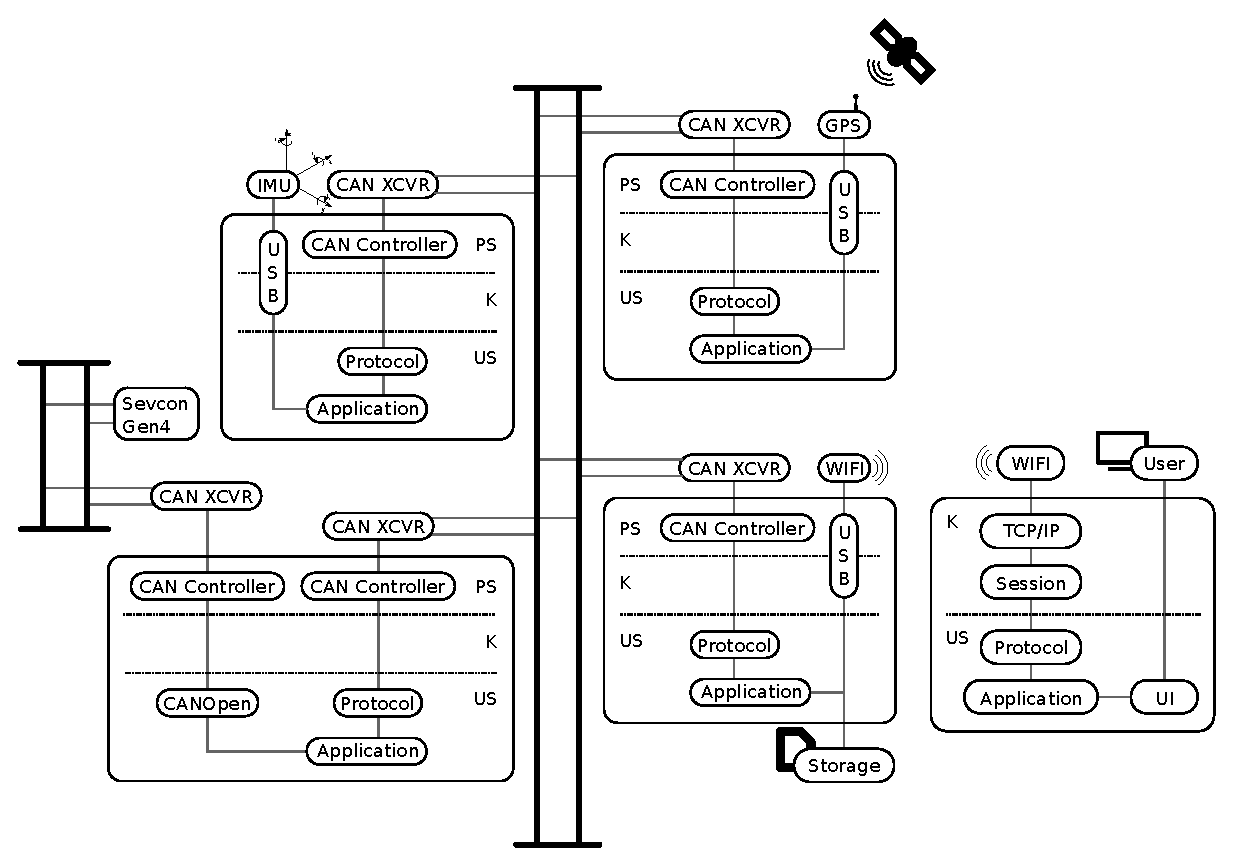
\includegraphics[angle=90,width=\textwidth]{graphics/analysis_complex.eps}
	\caption{The big system........}
	\label{fig:complete_system}
\end{figure}

% \subsection{Actors}
% The only actor on the system is an engineer.

% \subsection{Interfaces}
% \begin{itemize}
% \item Wifi, for data transfer between go-kart and stationary computer.
% \item CAN bus, for local network.
% \item CanOpen, for interfacing the Sevcon.
% \item USB, for GPS and IMU.
% \item ??, for SD card connection.
% \item Powersupply, for Zybo boards.
% \end{itemize}

% \subsection{Functional requirements}
% The system: 
% \begin{itemize}
% \item Reads data from sensors.
% \item Reads data from Sevcon.
% \item Transfers data to stationary computer using Wifi.
% \item Presents data to the user.
% \item Logs sensordata to SD card.
% \item Read data from SD card.
% \item Timestamps all data. 
% \end{itemize}

% \subsection{Operational requirements}
% The system monitors go-kart data.% when engineer starts the system by powering it on.

% \subsection{Quality of service requirements}
% \begin{itemize}
% \item IMU data must be sampled with xx Hz.
% \item GPS data must be sampled with zz Hz.
% \item Data logging with qq Hz.??
% \end{itemize}

% \subsection{Parametric requirements}
% Wifi range must be greater than xx meters.

% \subsection{Design requirements}
% The system:
% \begin{itemize}
% \item must be scalable to at least 16 sensors/nodes.
% \item must be modular to allow easy integration of new sensors/nodes.
% \item must be functional if one or more sensors/nodes stop working.	 
% \end{itemize}


% section system_requirements (end)
\newpage
\part{Implementation}
%!TEX root = ../main.tex

A node can be any kind of microcontroller, but this section will only address the case where a Zybo is used. 

Throughout the analysis a number of decisions were made regarding the hardware and technologies to be used in the realisation of the system.
These are outlined in section \ref{sec:analysisconclusion}.
It was found that it is necessary to implement two different networks, one for collecting the data on the go-kart and one for transmitting the data to a monitoring station, assumed to be a standard PC throughout the remainder of the report.
These two networks will be referred to as the on-vehicle and off-vehicle networks, respectively.
The implementation of these, along with the remainder of the system, is described in this part.
Should a user or developer wish to implement their own node, a guide exists in appendix \ref{app:addnode}, outlining the steps necessary to implement a node.
\thomas{Rewrite}
\mikkel{REMEMBER TO TELL THAT WE DO NOT HAVE ANY KIND OF REALTIME !!!!! SOMEWHERE THIS SHOULD BE DESRIBED !!}
\section{On-Vehicle Network}
%!TEX root = ../main.tex

\subsection{On-kart network}\label{sec:CANbus}
The CAN is described in this section, starting with the implementation of the physical layer.
After that, the CAN framework is described, and finally how this framework is used to create a protocol for this project

\subsubsection{Physical Layer}\label{sub:CANphys}
The physical layer has three main parts: The CAN controller, the CAN transceiver and the bus itself. \\

The Zybo supports CAN, and has a CAN controller in its PS.
An IP core is also available if FPGA implementation was desired.\\

The CAN transceiver is connected to the controller by Rx and Tx voltage signals, and connects to the bus through two differential ports. 
The transceiver must support the standard ISO11898-2, as this is what the Sevcon motor driver uses.
The device SN65HVD232 from Texas instruments support this standard, and is supplied with 3.3 V, so it can be plugged right into the Zybo, and still communicate with the Sevcon even though its CAN bus uses $\si{5 \volt}$.
According to TI itself\cite{3.3V_CAN}, this family of $\si{3.3 \volt}$ transceivers are compatible and interoparable with other \si{5 \volt} transceivers, so long as they support the same standard.\\

PCBs for the CAN transceivers are reasonably simple in design and while they can be procured, it was decided to create a custom transceiver.
This way it is possible to create a more mechanically solid stack.
The transceivers have been mounted on boards, that plug directly into the Zybo's 12-pin PMOD connector, which will be stacked on top of each other. 
The schematic is shown below.

\begin{figure}[h!]
	\centering
	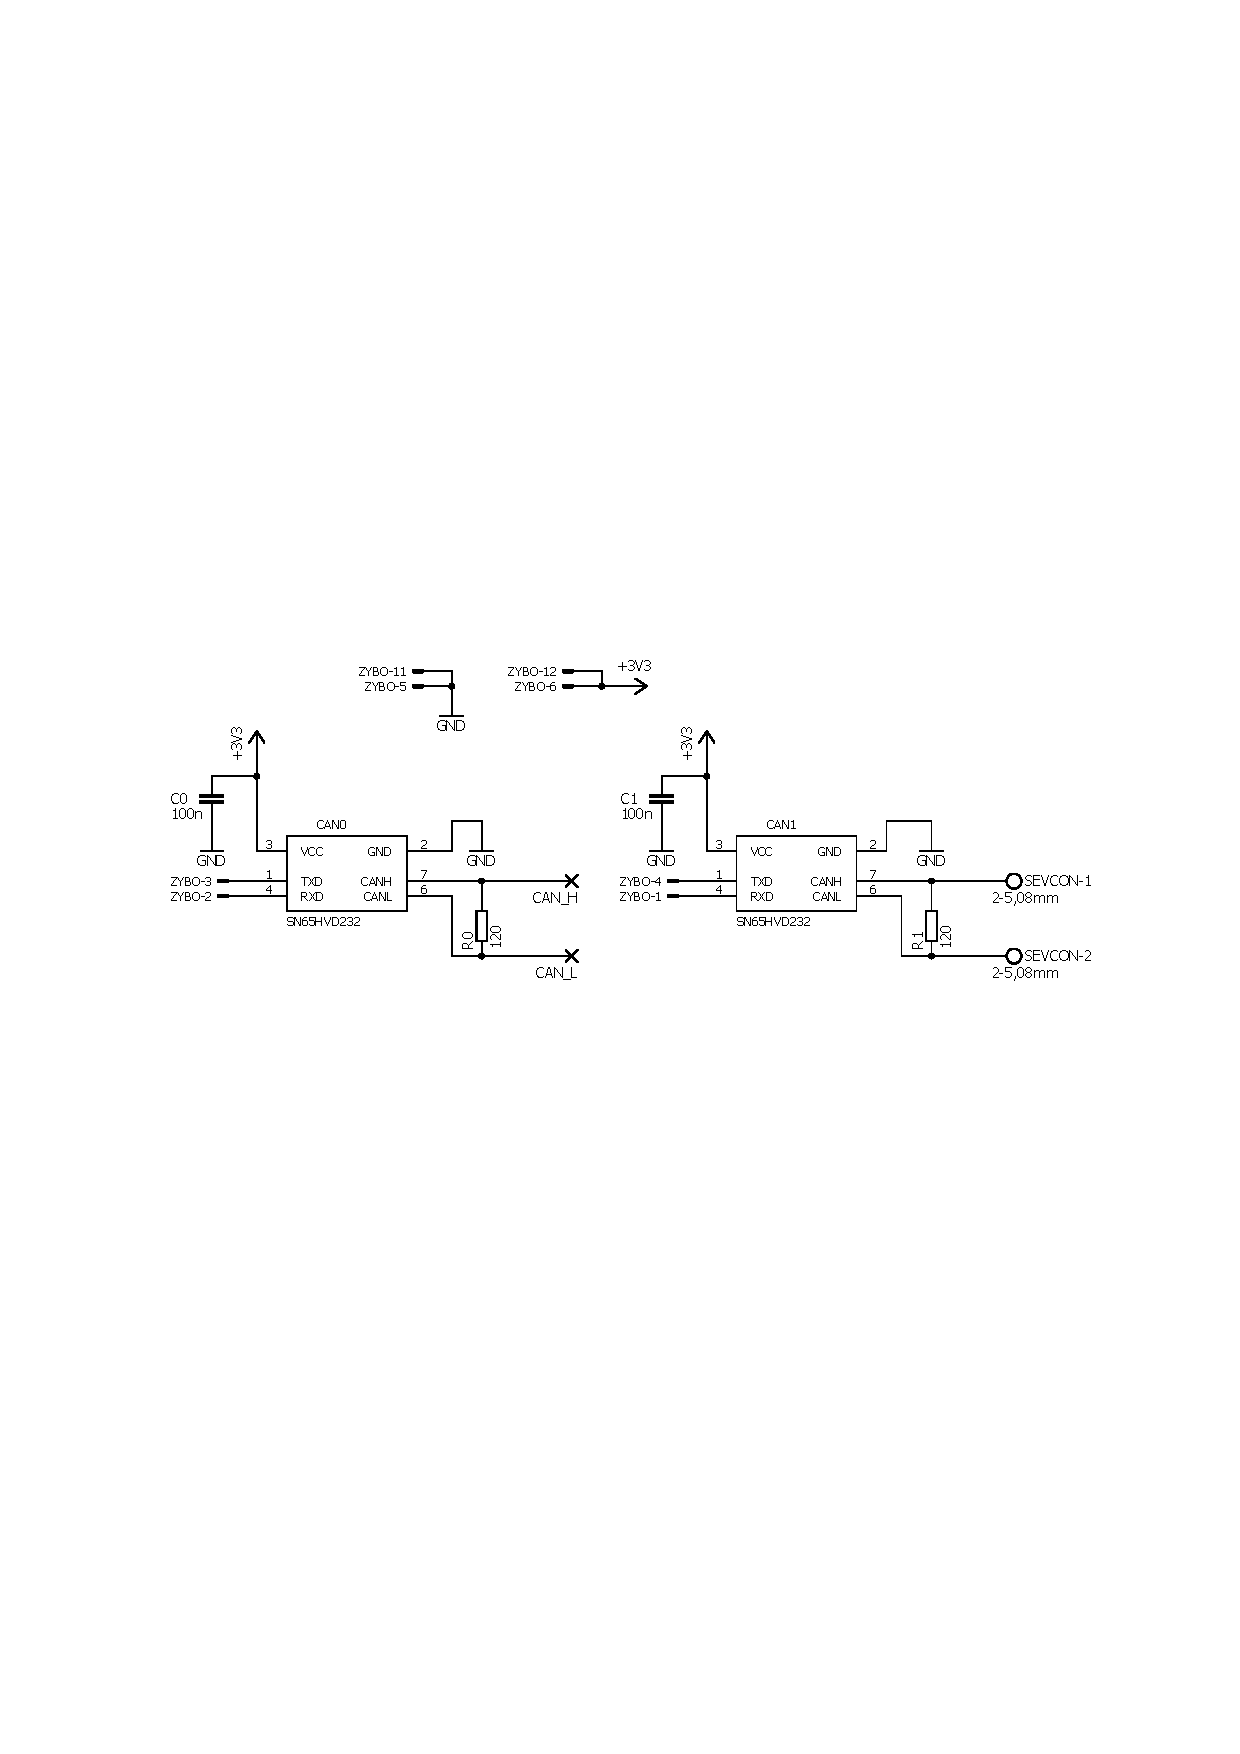
\includegraphics[width = 0.7\linewidth]{graphics/CAN_Schematic}
	\caption{Schematic of the two can transceivers. One board is build for two transceivers each with pads for termination}
	\label{fig:CAN_Schematic}
\end{figure}

The board has been designed to use the MIO ports, available in the PMOD JF. 
This is necessary to utilize the build in CAN controllers on the PS part of the Zybo.
Although the schematic contains two transceivers and two termination resistors, most of these devices are not mounted. 
Four boards will be made, all containing CAN0, C0 and the ZYBO connector. 
One board will also include the resistor R0 - this is the bottommost board
Another board will include R0, R1 CAN1, C1 and the SEVCON connector.
Ths is placed on top, to allow the SEVCON connector's screws to be accessible. 
The stack is visible below

\begin{figure}[H]
	\centering
	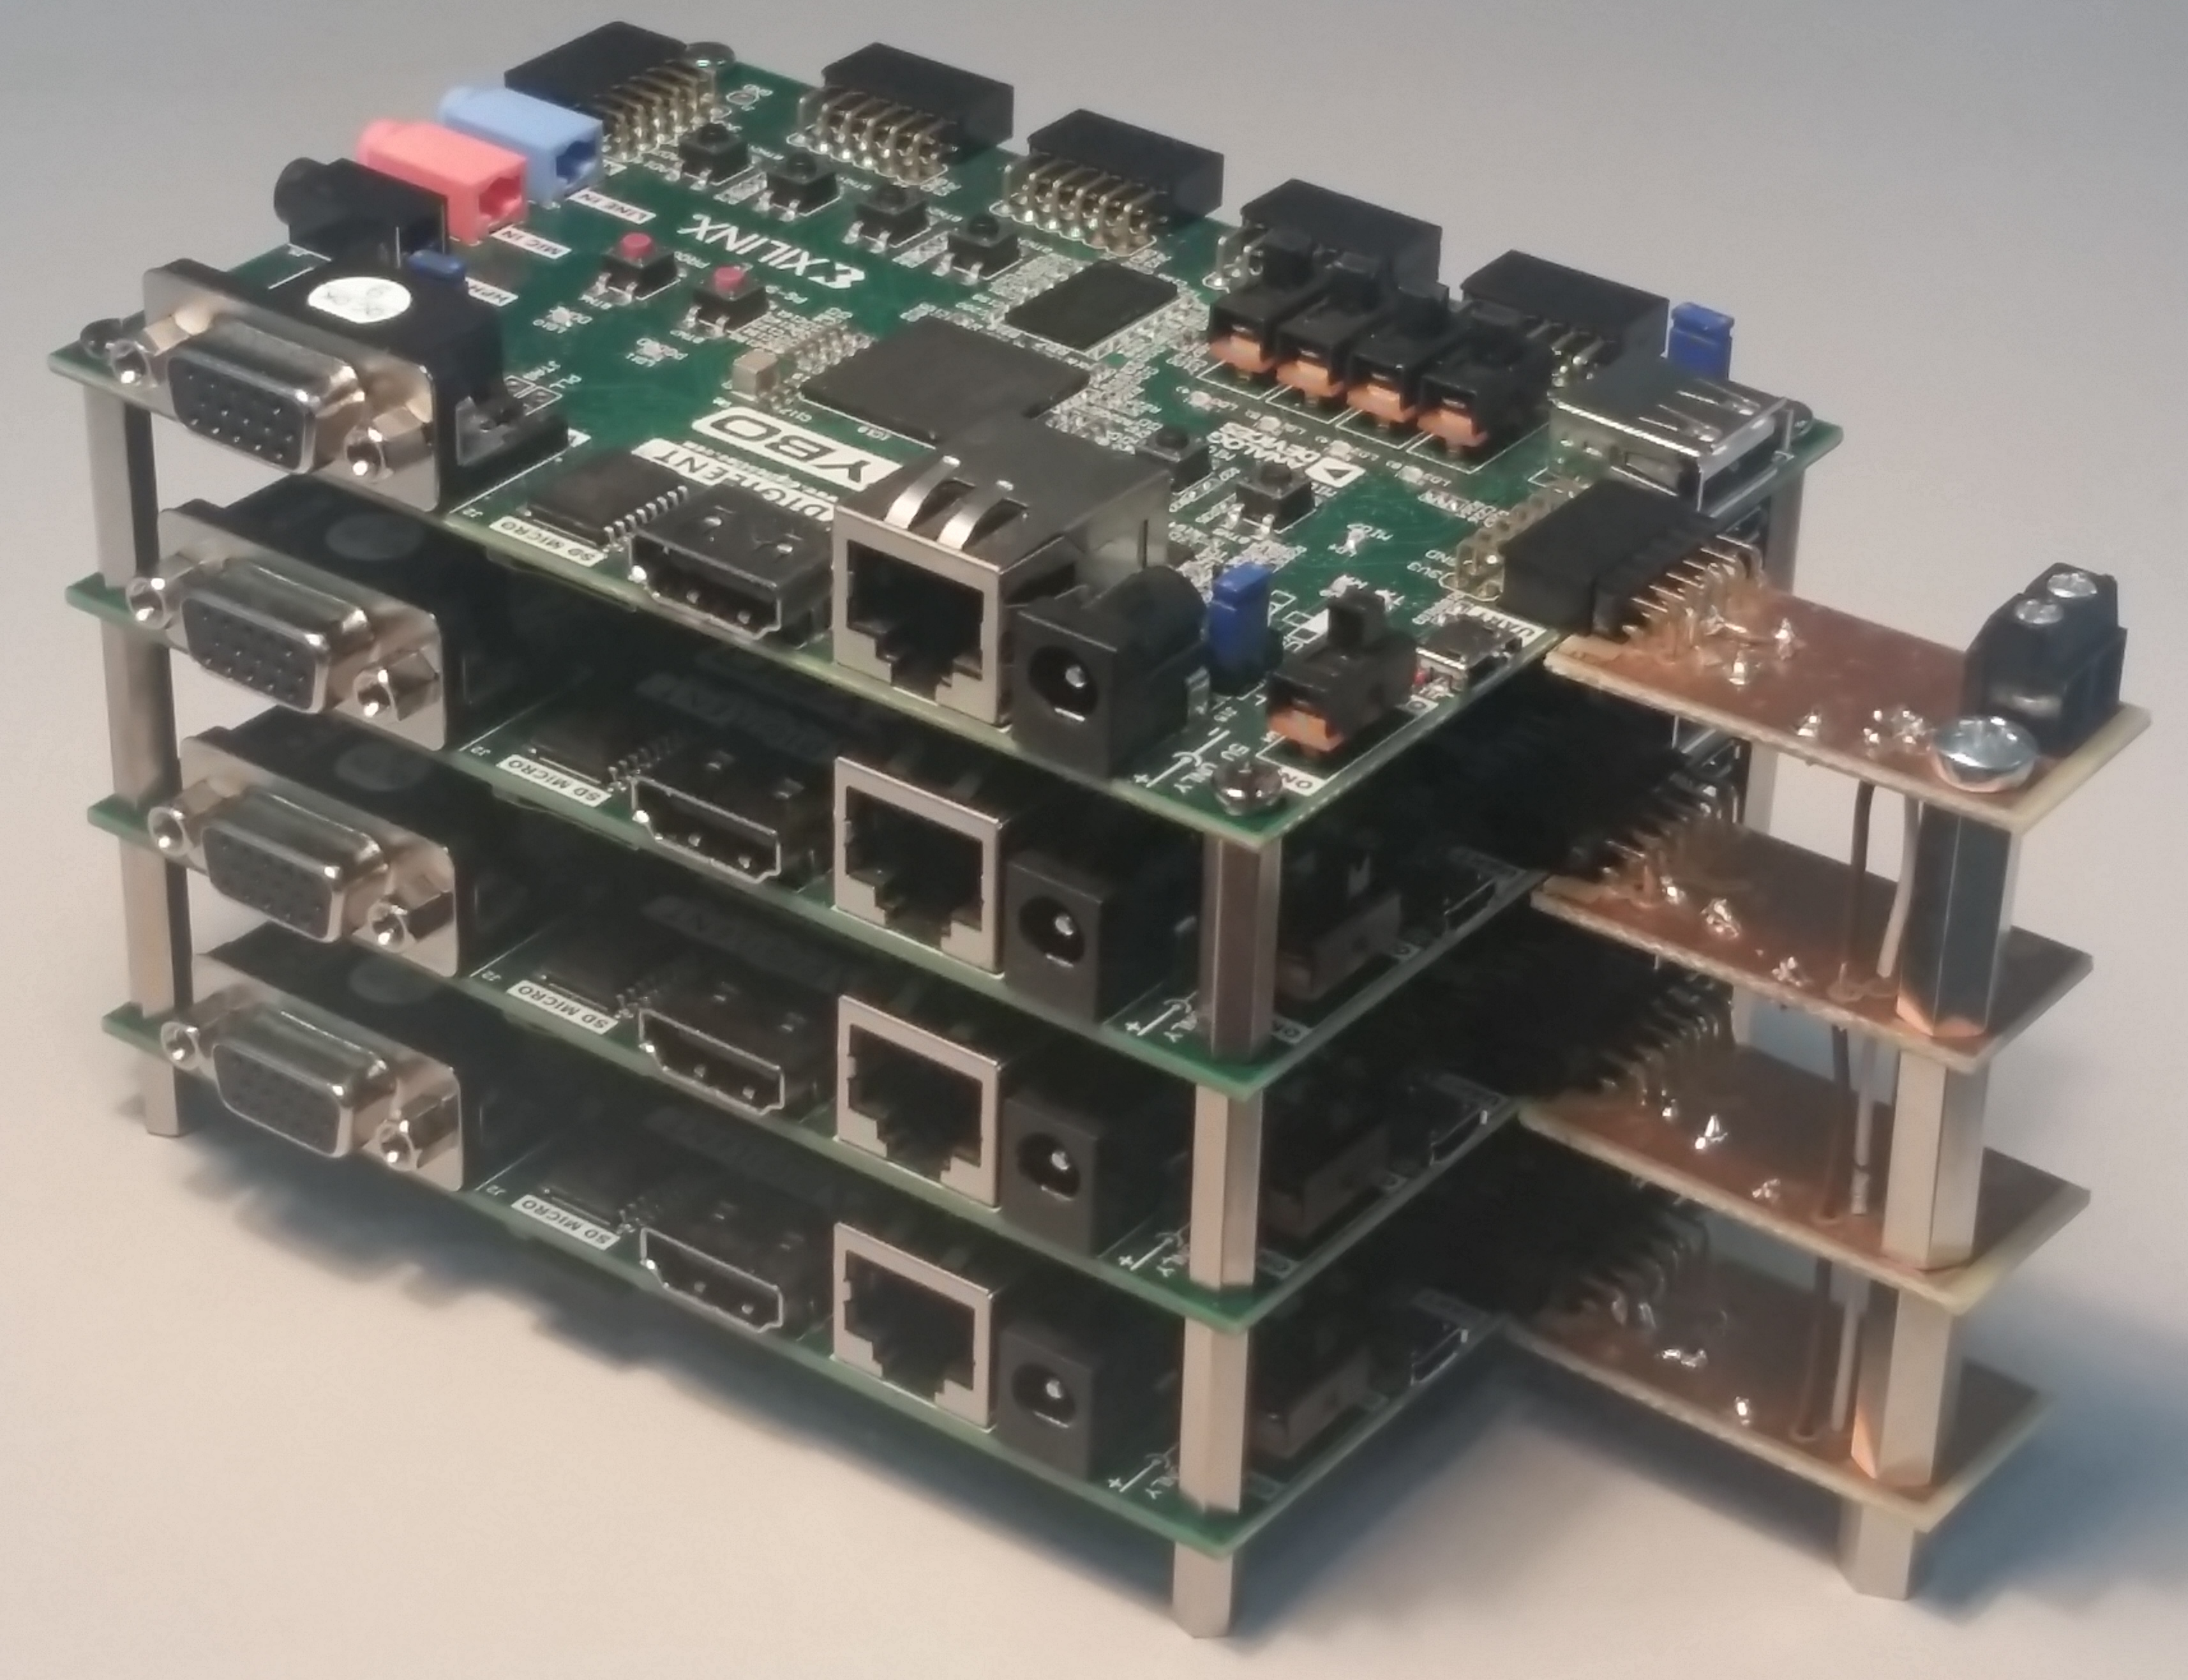
\includegraphics[width = 0.9\linewidth]{graphics/CAN_stack_picture}
	\caption{The CAN stack plugged into one Zybo}
	\label{fig:CAN_stack_picture}
\end{figure}

Because the bus is so short, it isn't practical to make twisted pair, and this will work fine.
The bus itself is also not $120 \si{\ohm}$, but experiment shows that it works.

\todo{Polish the text and re-express some things such as send() function...}

\subsubsection{CAN Message Frame}\label{sub:CanMessageFrame}
Messages sent over CAN is put into a frame. 
One frame contains all the parts in figure~\ref{fig:CAN_frame_pdf}, whereas a message should not be restricted to just 8 bytes -- however it doesn't include any overhead.
A zero input to the transceiver will result in a voltage difference on the CAN bus, and a one input will result in no difference. 
A zero will alway be dominant -- this is used to ensure that two nodes to not talk at the same time.
If a node tries to write a one, but simultaneously reads back a zero, it will know that something is wrong, for instance, that the bus is occupied by a node with higher priority.
The CAN message consists 47 bits of overhead with each message of 0-8 bytes. 
This overhead includes a such things as message IDs and checks, to ensure that the message is received correctly, and collectively this is called a frame. 
The frame of the message is described here.

\begin{figure}[h!]
	\centering
	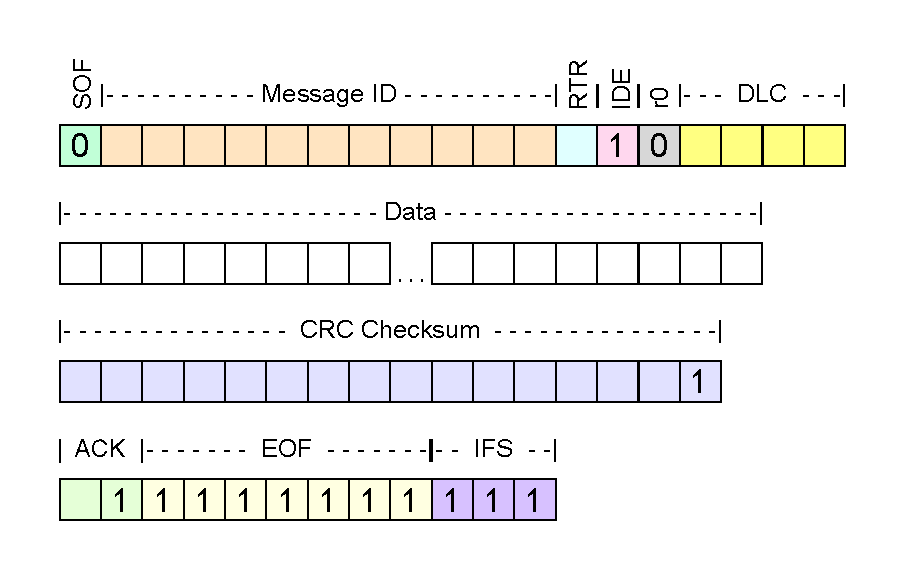
\includegraphics[width = 0.9\linewidth]{graphics/CAN_frame_pdf}
	\caption{Bitwise representation of a CAN frame}
	\label{fig:CAN_frame_pdf}
\end{figure}

\begin{itemize}
	\item SOF: \textbf{S}tart \textbf{O}f \textbf{F}rame: One dominant bit to start a frame.
	\item Message ID: 11 bit message identifier provides information about what the message contains. Subscribers will recognize a message by this ID.
	\item RTR: \textbf{R}emote \textbf{T}ransmission \textbf{R}equest: set to 1 if a transmission is requested from another node. Because is a publisher-subscriber network, this will always be 0.
	\item IDE: \textbf{ID E}xtended: Set to 1 if extended ID is in use. This adds 18 more bits of message identifiers immediately after this bit. At the moment, this is not needed, and should always be 0.
	\item r0: bit reserved for future use, alway set to zero
	\item DLC: \textbf{D}ata \textbf{L}ength \textbf{C}ode: how many bytes, of data, the frame contains. Ranging from 0-8.
	\item Data: Raw data. 
	\item CRC Checksum: \textbf{C}yclic \textbf{R}edundancy \textbf{C}heck: 15 bit checksum based on what was written in the Data portion. The last bit is a delimiter, and is always 1.
	\item ACK: \textbf{ACK}nowledge: The transmitting node will set the first bit of ACK to be recessive (1). Each receiving node will calculate CRC based on the data, and compare it to the CRC checksum. If no error is detected, it will set the bit to dominant (0). On a multi-node network, if one node confirms the data, the transmitting node cannot know if any other node did not receive the data. However, because of the nature of a differential voltage bus it is nearly impossible that two nodes would not receive the the same signal, so long as the bus is correctly impedance matched, and distances do not exceed the specification. The last bit o ACK is a delimiter, and always 1
	\item EOF: \textbf{E}nd \textbf{O}f \textbf{F}rame: Pattern signifies the end of a frame, the pattern is 7 recessive bits.
	\item IFS: \textbf{I}nter\textbf{F}rame \textbf{S}pace: an arbitrary length of recessive bits, at least three bits long. After this point, a new frame may start by setting a zero.
\end{itemize}

Because 0 dominates zero, it is possible to prioritize messages -- lower message ID get higher priority.
If two nodes start writing a message at the same time, the first node to write a 1 when the other node writes 0 will realize that another node has right of way, and will stop transmitting and wait for the current frame to end.
When the end of the message occurs, the node will try to send the message again.
It might then be blocked again by another node, and there is a risk, that it will never send.
It is the developer's responsibility to ensure that this doesn't happen.\\

It is, that messages are extended by bit stuffing.
If either 0 or 1 is written to the controller 5 consecutive times, the opposite polarity is interjected, or stuffed, into the stream. 
This is done to ensure that receiving nodes remain synchronized with the transmitting node, as there is no clock signal.
That means, that a frame can be extended by upwards of 20 \% if the data requires it.


\subsubsection{Testing the CAN Stack for a Basic Network}
\martin{This testing should be moved to the bottom of this section, to test the protocol as well}

After the design and printing of the stack board, testing it was the next step.
The test included using one the CAN controllers within the Zynq chip with the purpose of showing that a basic CAN network between two Zybo boards could be implemented using the stack.
Specifically, the one Zybo was sending the input value of the buttons to the network in order to be received by the second one and turn on the on-board LEDs as a result.
After designing a basic architecture in Vivado and writing a source code, the test was successful, thus proving the basic functionality of a CAN network.
All Zybo boards were programmed with the same architecture and source code.

\paragraph{Architecture}
In order to realize the above test, enabling the CAN controller inside the Zynq chip as well as including two AXI GPIO cores were necessary.
One AXI GPIO was setup as leds 4bits while the other one as btns 4bits as it can be seen in figure \ref{fig:CAN_Testing_Architecture}. The architecture was firmly simple, but adequate to meet the purpose of the test.

\begin{figure}[h!]
	\centering
	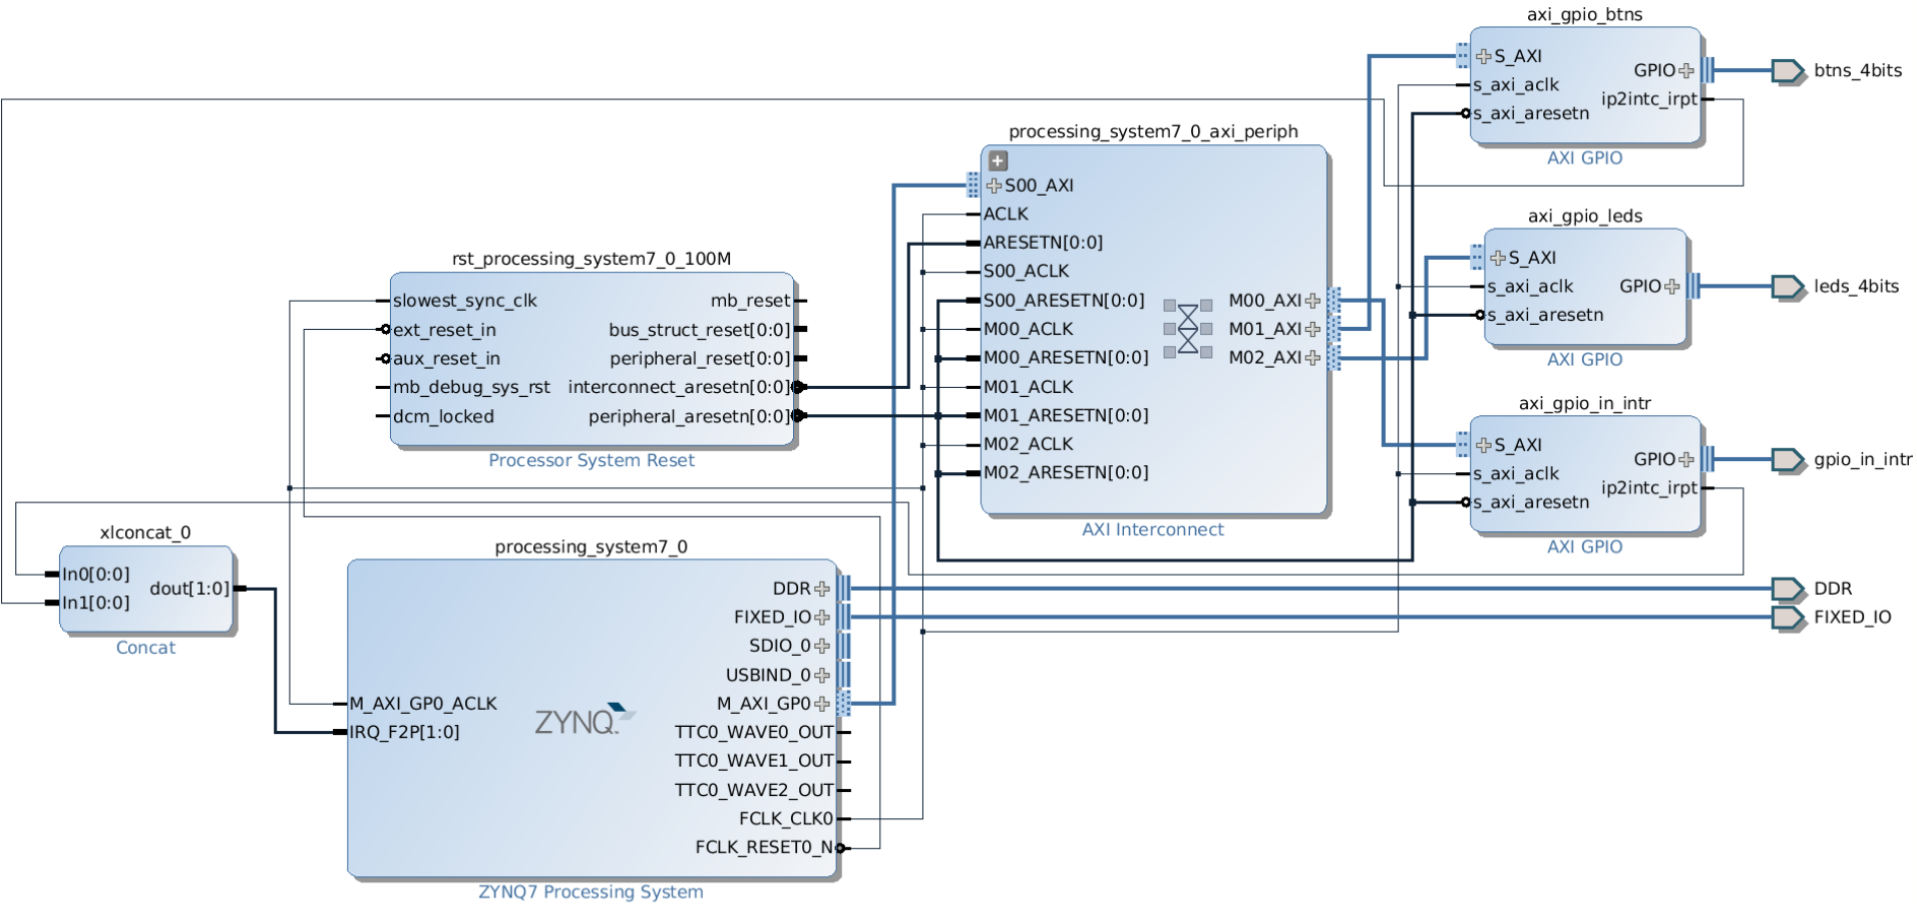
\includegraphics[width = 0.9\linewidth]{graphics/Zybo_BasicTestingArchitecture_for_CAN.png}
	\caption{Block diagram featuring the testing architecture in Vivado.}
	\label{fig:CAN_Testing_Architecture}
\end{figure}

\paragraph{Source Code}
The programming for this task was done in C.
The code from xcanps polled example provided by Xilinx documentation was used as a basis.
The example shows the basic principle of sending and receiving messages on a loopback network on a single board.
With further modifications and the addition of extra functionalities such as reading button input and writing the output to the LEDs, the finalized developed code was suitable to test the communication between two nodes on the CAN network.
\\\\
The basic principle for testing was to trigger an interrupt attached to the button presses, which then the send() function would send the value of the buttons to the network as a message.
In turn, the receive() function was responsible of reading the message transmitted on the bus and writing the value as output to the LEDs.
As mentioned before, this source code was common and uploaded to both boards resulting in a two-way communication, since both of them had a send() and a receive() function, thus one controlling the LEDs of the other one.

\todo{We need a picture with 2 or better, 4 boards as stack! The coolest thing ever :P.}

%!TEX root = ../main.tex

\subsection{Go-Kart CAN protocol (GoCAN)}\label{sub:CAN_protocol}
Due to the requirements of the on-kart network, it was decided to formulate a new protocol specifically for this project.
While CANopen could be used, it is a vast protocol with many features that are of no use in this system.
An elaboration of the choice to make a custom protocol over using CANopen is done in this section.
Additionally, the design of the go-kart CAN protocol, or GoCAN for short, is also presented.
The requirements of GoCAN are listed below.

\begin{itemize}
	\item Simple and easy to learn.
	\item Support for 16 nodes.
	\item One node must be able to receive/transmit data to/from multiple inputs/outputs
	\item Publish/subscribe architecture.
	\item Variable data length - beyond 8 bytes per message
	\item Expandable -- must be able to add more nodes without affecting the existing ones.
	\item Commands: Start/stop broadcasting 
	\item Commands can be send to specific or all nodes
	\item Timestamp data
\end{itemize}

\thomas{This is changed!}
\subsubsection*{The CANopen Protocol}
\label{sub:CANopen}
As mentioned before, CANopen is a high level protocol that runs on top of the CAN protocol.
It is open source project, that runs on the top 5 layers of the OSI model\cite{CANopen_introduction}.
It includes several types of protocols, most interesting are the SDO and PDO. 
By splitting the 11 bit Message ID into a 4 bit function code, followed by 7 bits of node ID, meaning that a node can communicate 16 different functions to 127 different nodes.
\\~\\
The Service Data Object (SDO) can read from or write to any registers on any node. 
It can handle 127 different nodes with each 65536 different indices, each with 256 sub indices, in total, more than 2 billion addresses with each 4 bytes of data.
The way CANopen supports this, is by using the first four bytes of the data portion of the frame for metadata, as described in figure~\ref{fig:CANopen_SDO_data}.

\begin{figure}[h]
	\centering
	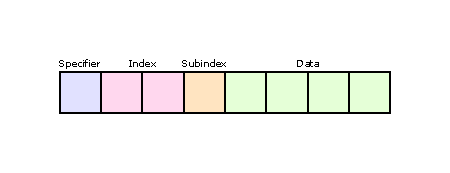
\includegraphics[width=0.9\linewidth]{graphics/CANopen_SDO_data}
	\caption{"The data section of the CAN frame is split into three parts: one byte for the specifier, three bytes for the node index and subindex, and four bytes for the actual data in the transfer."\cite{CANopen_introduction}}
	\label{fig:CANopen_SDO_data}
\end{figure}
\thomas{de-jesusify}

\martin{Clarify facts}
This of course means that the overhead from one message increases from 47 bits to 59 bits, or 184 \% of the maximum data size.
\\~\\
This protocol is not ideal for this network. 
In part because it's request based, but more because of the enormous overhead.
The IMU would produce 999 bits in order to transmit its 9 axis data without loss of precision, and at 400 Hz, that node alone will take up 40 \% of the bandwidth.
In addition to this, all transmits would need to be requested, so the total bandwidth comes close to 70 \%.
%Metadata is 47 bits, plus 32 bits from the Data portion. The data it self is a float, so that's 32 bits; 111 in all. A request does not include data, so that's only 79 bits of data. At 400 Hz, that's (111+79)*9*400=684000.
The SDO is generally used to define or read parameters for that node, that are not bound to change over time.
It should not be used for broadcasting data.
\\
The Process Data Object (PDO) is a protocol used to transmit specific indices with a higher throughput. 
In this protocol, certain indices are mapped to one of 8 PDOs. 
This way, a node can identify data only by the CAN message ID, without using any of the data portion for overhead.
It is also possible to group multiple values together, and to transmit without request -- either at fixed time or event driven.
This brings the data from the IMU down to 523 bits to transmit its 9 axis data.\\
%((32+32)+47)*4+(47+32)

Each node on the CANopen bus has its own Object Dictionary (OD) specifying its addresses. 
Some of these addresses are reserved, but since the Message ID specifies which node it is, there's no risk of overlapping.
If then one part is replaced by a different make or model, then it might be necessary to reconfigure other nodes, and the system loses modularity.\\

For all its nice features, the CANopen protocols do not fit the requirements outlined in the beginning of this section. 
It includes a lot of complexity, which unnecessary for this project.
Instead it has been decided to develop a custom High Level Protocol that relies more on the automatic functionality of the CAN protocol.\\

\subsubsection*{The GoCAN Protocol}
The basic CAN frame is retained for this protocol.
GoCAN, mostly, is a reinterpretation of the message ID of the frame.

\begin{figure}[h!]
	\centering
	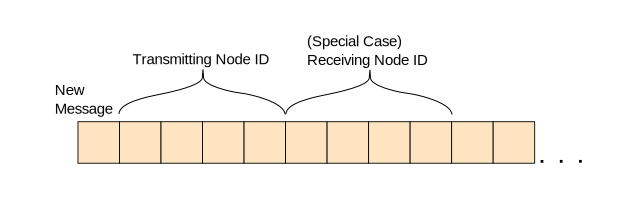
\includegraphics[width = 0.9\linewidth]{graphics/CAN_protocol_general}
	\caption{Naming convention for this high level protocol}
	\label{fig:CAN_protocol_general_pdf}
\end{figure}
\thomas{Indicate messageid, remove color in dotted box, split into two cases}
The message ID is split into three portions, as seen on figure~\ref{fig:CAN_protocol_general_pdf}.
The first bit is set to 1 if this is a new message.
If the node needs to send more than 8 bytes in one message, this bit can be set to 0, thus blocking other nodes with higher priority.
The subsequent four bits indicate the transmitting node ID, which will allow up to 16 nodes. 
The last 6 bits of the message ID determine the message type. 
This leaves 64 different message types for each node.
It is the responsibility of the developer to utilize these correctly.\\

There are two types of nodes: 
\begin{itemize}
	\item \textbf{The Wifi node:} Acts as the link between the user on the monitoring station and the network.
	It transfers data to the monitoring station and distributes commands on the network.
	\item \textbf{Sensor nodes:} Any sensor or data producing unit will be associated with a node.
	A sensor node will produce data and act according to received commands
\end{itemize}


In this case, the subsequent four bits determines the recipient, leaving two bits for command type. 
For now, command types are "Start broadcasting", "Stop broadcasting" and "Synchronize".
These will be explained in more detail in section \ref{sec:CAN_functions}.
If the recipient message ID is the WiFi node ID, then the command applies to all nodes.\\
\thomas{Reference to figure msg id}

The four node IDs currently in use:
\begin{table}[h]
	\begin{tabular}{{l} {l}}
		Wifi node: & 0b0001 \\
		IMU node: & 0b0011 \\
		Sevcon node: & 0b0111 \\
		GPS node: & 0b1110
	\end{tabular}
\end{table}

The WiFi node is given the lowest node ID since this will result in the highest priority.
This is necessary when issuing commands.
The IMU produces short data packages at a high rate, and the GPS node produces data packages at a lower rate. 
Therefore it is of less concern if the GPS message is delayed due to obstruction from other nodes. 

%!TEX root = ../main.tex
\subsection{Functions of the CAN protocol}\label{sec:CAN_functions}
Some added functionality is necessary for the High Level protocol, which will increase the usability of the protocol.

\paragraph*{Timestamps}
As mentioned in section~\ref{sec:CAN-bus} the CAN protocol is not real time, which means all data on the bus must be timestamped. 
This way, the latency of each data point will be known, and it would be possible to work with data fusion.
The resolution of the timestamps has been decided to be 1 ms, as this leaves sufficient accuracy for the sensors analysed in this project.
This presents several challenges, in terms of what the time reference is and how to convey timestamps with adequate precision without creating too much overhead. 
For a node running Linux, the Epoch timestamp is available, but this is not available on baremetal code - it is also too coarse, as it only updates every second.
Instead a counter will be implemented on each node, incrementing an s32 integer every 1 ms.
This gives 24.8 days before overflowing.\\

Because a standard s32 integer takes 4 bytes, it would introduce a large overhead if the timestamp is sent with every message. 
Instead, each timestamp will determine the time of all subsequent data messages, until a new timestamp is sent. 
As an example, the pseudo code below describes the transmission of all nine axes of the IMU with the same timestamp.
Additionally, the IMU can transmit pressure and temperature measurements, but as these are slower signals, they would be transmitted at a lower rate.

\begin{lstlisting}
Send Timestamp
Send Ax, Ay, Az
Send Gx, Gy, Gz
Send Mx, My, Mz
Wait
Send Timestamp
Send Ax, Ay, Az
Send Gx, Gy, Gz
Send Mx, My, Mz
Send Pressure, Temperature
Wait
\end{lstlisting}

Lines 2-4 are measurements taken at the timestamp in line 1.
The WiFi node then saves each of these nine data points with the corresponding timestamp.
Lines 7-10 refer to the timestamp at line 6.\\
Because of the Tx Fifo in the CAN controller, it is possible to build and send four or five frames simultaneously, and let 


\paragraph*{Commands}

\paragraph*{Synchronization}

\paragraph*{Multiframe Messages}

\paragraph*{Datatype and Scaling}


\subsection{CAN Controller Software}
\catalin{Explain the code in more detail. Also mention the interrupt part for gpio.}
\catalin{Bullet list: What other functionalities? And, 1st letters capitals or not?}
\catalin{Better titles}
\martin{Write introduction explaining that this code is for testing, because we were missing the link betwen linux and CAN.}
\subsubsection{Main Functionalities}~\\
As mentioned in section \ref{sub:Basic_SourceCode}, the code was based on the xcanps polled example available by Xilinx documentation.
The important functionalities that needed to be provided by the final software version included:
\begin{itemize}
\item receiving and sending of frames
\item creating the message id
\item decoding of the message id parts, such as the node id, the message type and the command
\item handling interrupts from buttons and a GPIO port
\item controlling the LEDs
\martin{buttons and leds aren't part of the final software? Or are we still talking about the software for testing?}
\item accepting and ignoring messages according to a subscriptions list
\end{itemize}

\subsubsection{Publisher-Subscriber Architecture}
\catalin{Should I explain more about the architecture? Or is it the readers responsibility to read about it?}
A mechanism was also necessary to control the receivers and transmitters of messages.
One of the functionalities of the network was to provide the ability for various nodes to be able to send specific messages to other nodes.
Such a mechanism could easily be implemented using the Publisher-Subscriber architecture which would also make the network data-driven.
Using this method, the communication among the various nodes could be easily configured just by adding messages ids to an array variable containing the node's subscriptions.
The use of this architecture was incorporated in the protocol functionality, along with a set of functions in the source code and an array variable of subscriptions for each node.

\subsubsection{Main Loop}
Since the whole system, that was intended to be designed for this project, could not be put together, an approach to simulate the network in various ways was needed.
Specifically, sending arbitrary messages was achieved by implementing button interrupts
%\martin{I removed some text, that doesn't fit with the validation part}
%and the case where multiple nodes would send messages simultaneously by GPIO port interrupts.
%For details on how the different tests were done the reader may refer to section \ref{sub:CAN_Bus_Tests}.
%Due to conflicts between the interrupt controllers and handlers, only one of the two simulation cases could be active during runtime.
%Depending on the value of a macro definition in the source code the desired devices (buttons or GPIO) would be initialized.

\paragraph{Button Interrupts Runtime}~\\
As seen in behavioral diagram in figure \ref{fig:FlowChart_CANSoft_BtnsIntr}, the program waits for button pushes or for receiving data in the FIFO in the main loop.
In the former case, a message is sent to the network containing the value of the pushed buttons, while in the latter case, the data is decoded and the appropriate value is written to the LEDs as output.
\begin{figure}[h!]
	\centering
	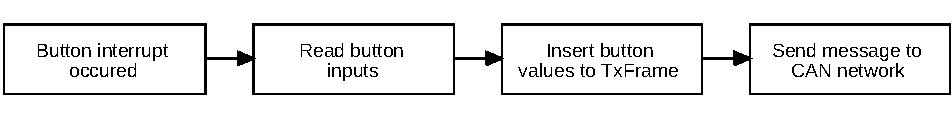
\includegraphics[width = 1\linewidth]{graphics/FlowChart_CANSoft_BtnsIntr.pdf}
	\caption{Behavioral diagram with button interrupts.}
	\label{fig:FlowChart_CANSoft_BtnsIntr}
\end{figure}
\begin{figure}[h!]
	\centering
	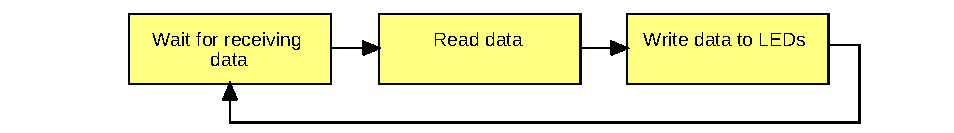
\includegraphics[width = 1\linewidth]{graphics/FlowChart_CANSoft_RecvData.pdf}
	\caption{Behavioral diagram with button interrupts.}
	\label{fig:FlowChart_CANSoft_RecvData}
\end{figure}

\paragraph{GPIO Interrupts Runtime}~\\
\martin{Do we use this? I didn't use interrupts for my code}
The software's behavior is similar in this case, as well as it can be seen in figure \ref{fig:StateDiagram_CANSoft_GPIOIntr}.
The difference is that instead of button values, dummy data may be inserted into the TxFrame according to the simulation needs and the receiving data is only presented in the SDK terminal.
\begin{figure}[h!]
	\centering
	
\includegraphics[width = 1\linewidth]{graphics/FlowChart_CANSoft_GPIOIntr.pdf}
	\caption{Behavioral diagram with GPIO interrupts.}
	\label{fig:FlowChart_CANSoft_GPIOIntr}
\end{figure}

\subsubsection{Sending and Receiving Frames}
\martin{We probably should document something about the xcanps examples used in the verification}
\martin{Describe createMsgID()?}
The figure \ref{fig:SeqDiagram_SendFrame} shows the procedure of sending a frame to the CAN network containing data, which makes use of the protocol function createMsgID().
After returning the message id, the id and the data are put into the TxFrame to be sent once the FIFO has space.
The actual sending is done with a call to the XCanPs function XCanPs\_Send().
\\
Similarly, the procedure of receiving a frame is shown in the figure \ref{fig:SeqDiagram_RecvFrame}.
The node once it calls the RecvFrame() function, it waits in a loop until it receives a frame.
Then, it checks the subscriptions in order to forward the packet for further processing or to ignore it.
In both cases appropriate messages using the function xil\_printf() are presented to the developer in the SDK terminal.

\begin{figure}[h!]
	\centering
	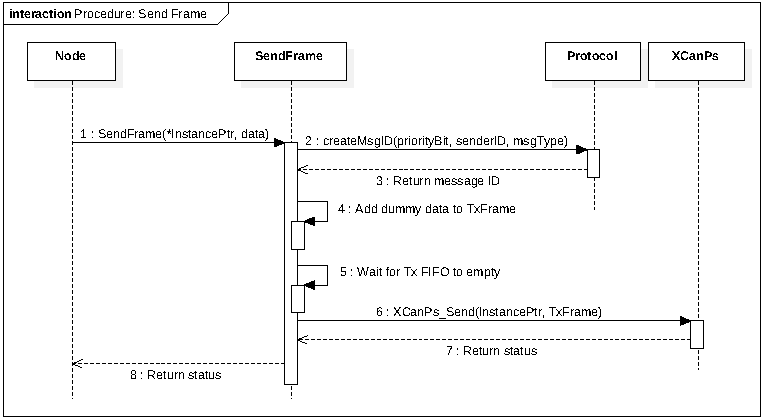
\includegraphics[width = 1\linewidth]{graphics/SeqDiagram_SendFrame.pdf}
	\caption{The sequence diagram of the process of sending a frame.}
	\label{fig:SeqDiagram_SendFrame}
\end{figure}

\begin{figure}[h!]
	\centering
	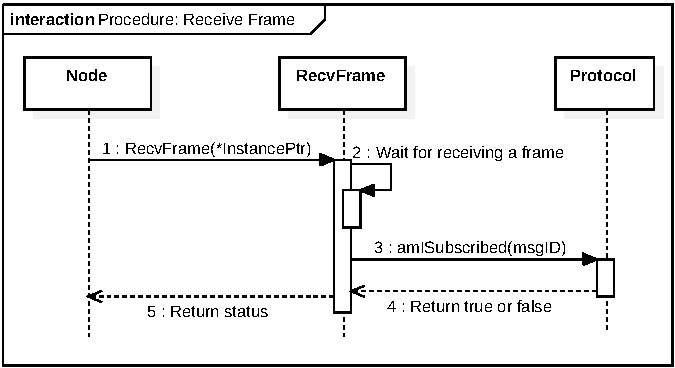
\includegraphics[width = 1\linewidth]{graphics/SeqDiagram_RecvFrame.pdf}
	\caption{The sequence diagram of the process of receiving a frame.}
	\label{fig:SeqDiagram_RecvFrame}
\end{figure}
%!TEX root = ../main.tex
\subsection{Methods to implement CAN on Linux}
\catalin{IMPORTANT: In case we get the actual network running, don't forget to change the text accordingly (implementation not successful etc.)}

The next step after testing the stack board and showing the basic functionality of the CAN network was to implement it using Linux running on the Zybo board.
\martin{It should be mentioned either here or before why it is necessary to implement on Linux as opposed to bare metal.}
This step required enabling the CAN drivers that reside in the Xillinux kernel and gaining access to the CAN devices.
\martin{The can controllers do not have anything to do with xilinux. Does Xilinux provide drivers for the can controllers on the zynq?}
This section describes the necessary procedures that were followed in order to gain control over the CAN network from Linux.
\\
At this point the reader should be informed that although the CAN controllers could be used on the Processing System using bare-metal code, the implementation of CAN on the Programmable Logic and the access to it from Linux was not successful.
\martin{Access to xcanps from Linux, design our own can controller on FPGA, asynchronous mode.}
After a lot of effort to create a physically functional network and researching on how to implement it, the conclusion that the available documentation is lacking was reached.
Alternatively, other means to prove the concept of the project were taken into account, as described in section \ref{sub:Utilizing_Svr_Virtualization}.

\subsubsection{Enabling the CAN Drivers}

This was the first idea on how to utilize the CAN network using Linux.
In order to enable the drivers on the Zynq7 Processing System, the Linux CAN driver guide \cite{Xilinx_wiki_Linux_CAN_driver} was followed.
The Kconfig file under the path \ref{code:can_kconfig_pathfile} needed to be configured.
The entry at line 128 was changed as seen in the code snippet \ref{code:can_kconfig_contents_line128}.
Originally, lines 130 and 131 were as seen in the snippet \ref{code:can_kconfig_original_line130}.
\martin{I think the original code snippet is irrelevant.}

\begin{lstlisting}[caption={CAN Kconfig pathfile.},numbers=none,label=code:can_kconfig_pathfile]
/usr/src/kernels/3.12.0-xillinux-1.3/drivers/net/can
\end{lstlisting}

\martin{Careful about the line length in the code}
\begin{lstlisting}[firstnumber=128,caption={Kconfig file contents from line 128.},label={code:can_kconfig_contents_line128}]
config CAN_XILINXCAN
	tristate "Xilinx(*@ @*)CAN"
	depends on NET [=y] && CAN_DEV [=y] && CAN [=y] && (ARCH_ZYNQ || MICROBLAZE [=y])
	default y
	---help---
	  Xilinx CAN driver. This driver supports both soft AXI CAN IP and
	  Zynq CANPS IP.
\end{lstlisting}

\begin{lstlisting}[firstnumber=130,caption={Original content of lines 130 and 131.},label={code:can_kconfig_original_line130}]
	depends on CAN && (ARCH_ZYNQ || MICROBLAZE)
	default n
\end{lstlisting}

The next step of the process was the modification of the device tree settings file, requiring an entry for the CAN PS to be inserted.
The necessary file was located under the boot folder named as seen in \ref{code:dts_file_zybo}.
The modifications can be seen in the snippet \ref{code:dts_changes_zybo} for can controllers as well as for the AXI CAN core.

\begin{lstlisting}[numbers=none,caption={Device tree settings file and its path.},label={code:dts_file_zybo}]
/boot/xillinux-1.3-zybo.dts
\end{lstlisting}
\catalin{Double quotes are problem here as well. FIX THEM WHENEVER}
\begin{lstlisting}[caption={Device tree settings changes.},label={code:dts_changes_zybo}]
zynq_can_0: can@e0008000 {
        compatible = xlnx,zynq-can-1.0;
        clocks = <&clkc 19>, <&clkc 36>;
        clock-names = can_clk, pclk;
        reg = <0xe0008000 0x1000>;
        interrupts = <0 28 4>;
        interrupt-parent = <&intc>;
        tx-fifo-depth = <0x40>;
        rx-fifo-depth = <0x40>;
    };
axi_can_0: axi-can@40000000 {
        compatible = xlnx,axi-can-1.00.a;
        clocks = <&clkc 0>, <&clkc 1>;
        clock-names = can_clk,s_axi_aclk;
        reg = <0x40000000 0x10000>;
        interrupt-parent = <&intc>;
        interrupts = <0 59 1>;
        tx-fifo-depth = <0x40>;
        rx-fifo-depth = <0x40>;
        };
\end{lstlisting}

\mikkel{Maybe you can provide some thoughts about the problem. Maybe also some words about the patching Xilinx-Digilent etc.}
As was previously mentioned, the implementation was unsuccessful. At the time, the research done on this topic did not lead to successfully enabling the drivers.

\subsubsection{Utilizing the AXI CAN core}

Another way to implement a CAN network was to use the AXI CAN core that is available in the Vivado Suite, instead of utilizing the CAN controllers on the Zynq.
Unfortunately due to a license restriction from Xilinx, the core can only be used for simulation purposes and not actual hardware implementations.
This information became available after the process of generating the bistream file in the form of an error, thus not allowing for further use of the core.
The architecture can be seen in figure \ref{fig:CAN_Arch_with_AXI_CAN}.
The core accepts a clock frequency from \SI{8}{\mega\hertz} to \SI{24}{\mega\hertz}, which in the block diagram is provided by the FCLK\_CLK1.
\martin{Is the clock input relevant? As I see it, it would be more relevant to know if it can operate at 8 MHz to the transceivers.}

\begin{figure}[h!]
	\centering
	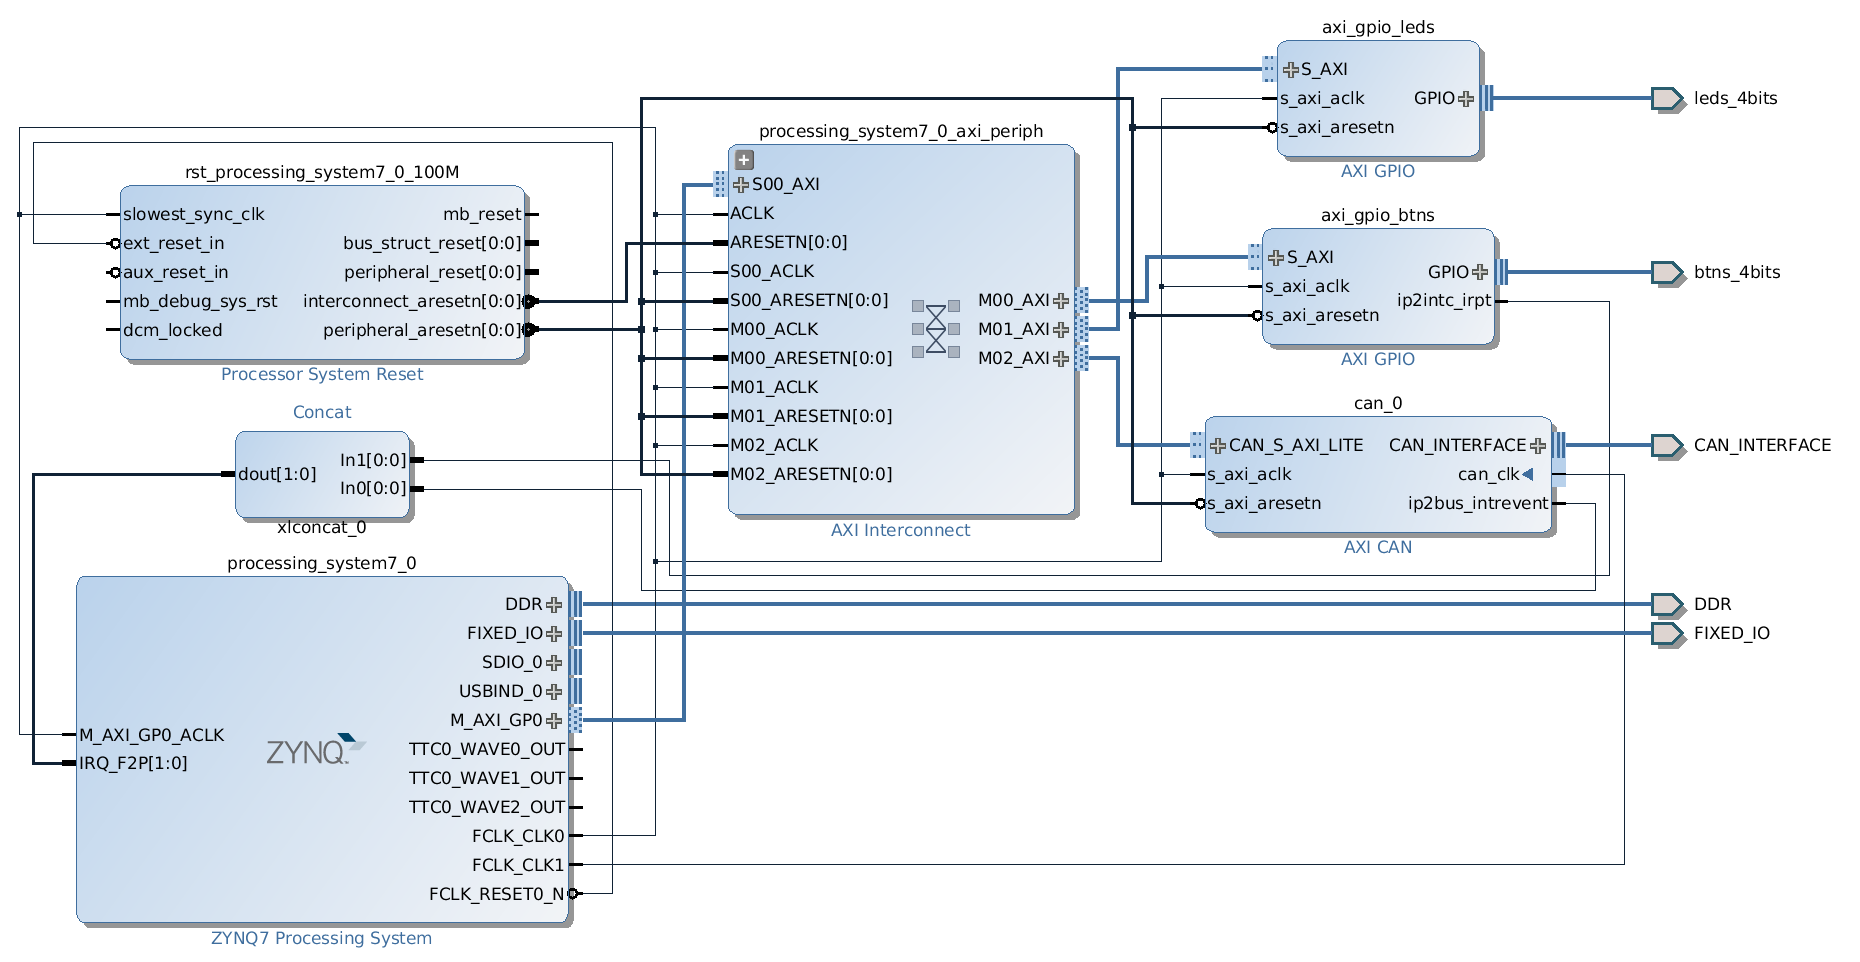
\includegraphics[width = 1.2\linewidth]{graphics/Zybo_Arch_with_AXI_CAN.png}
	\caption{Block diagram featuring the architecture in Vivado with the AXI CAN core.}
	\label{fig:CAN_Arch_with_AXI_CAN}
\end{figure}

\subsubsection{Utilizing Asymmetric Multiprocessing}

Apart from using the AXI CAN core and the CAN drivers, the Zynq-7000 AP SoC provides the possibility of implementing a mechanism called asymmetric multiprocessing since there are two processors which share common memory as well as peripherals.\\
\martin{CAN controllers instead of CAN drivers?}

The idea of this is to run Linux OS on one processor, while on the other one a bare-metal system, which both of them can communicate with each other.
This was a proposed solution for the problem of accessing the CAN devices from Linux which was the most promising of the implementation methods discussed in this report, but due to lack of time, it was researched only at a theoretical level.
\\
A brief implementation description will be given in this section, but for more details about the instructions and applications, the reader may refer to the Xilinx document \cite{Xilinx_AMP}.

\paragraph{Short Implementation Description}~\\
In order to achieve asymmetric multiprocessing on the Zybo board, certain steps are required to be taken, but also a few precautions as well.
An important one is to configure the two processors appropriately in order to use the shared memory without conflicts.
A second one is to setup the CPU0 as the master, because that is the processor assigned for the Linux OS.
It is also the one that will start CPU1 by writing a value to a specific address in memory.
\\
Linux also needs to be configured as symmetric multiprocessing with a maximum number of one CPUs.
It is a good approach because it will ensure that Linux configures the interrupt control distributor (ICD) and the snoop control unit (SCU) appropriately for multi-CPU environment, but only running on one of the two CPUs.
\\
Applications for the bare-metal and the Linux part are needed as well. Specifically, the former makes use of the fist stage boot loader (FSBL) as well as a custom application that will run on the CPU1 after it will be loaded by the FSBL into the memory.
The latter, the Linux OS, uses two applications as well.
The first one is RWMEM which is a utility providing the ability to read and write to various memory locations.
The second one is the Soft UART, which constantly monitors the memory in order to receive data from the application running on the second processor, the bare-metal code.
\\
The next step is to create the Linux kernel and device tree, as well as the u-boot.
\martin{So we need to build a new kernel anyway, which was also the brick wall we hit when trying to access the CAN controllers straight from Linux?}
Acquiring the root file system is also a requirement.
One important note here is the modification of the device tree includes instructions for the Linux to only use one CPU and to not access certain amount of memory, which is reserved for the bare-metal application.
For instructions for the creation of the kernel, u-boot and acquiring the root file system, the reader may refer to the Xilinx Wiki \cite{Xilinx_wiki}.\\
\martin{I don't think we should refer to the whole xilinx wiki. Specific articles or nothing}

Lastly, after all the above steps, the last one is to follow the appropriate procedures to copy the necessary files to an SD card. The files, including the applications, are:
\begin{itemize}
\item BOOT.BIN
\item uramdisk.image.gz
\item devicetree.dtb
\item uImage
\item rwmem.elf
\item softUart.elf
\end{itemize}

The application for the CPU1 is included in the BOOT.BIN file.
\martin{How big a task would it then be to change the baremetal code?}

\subsubsection{Using can-utils for virtual nodes}

During the development of this project, the can-utils tool was also used.
It is a testing tool that can be executed on Linux and can be applied on real as well as virtual CAN devices.
Initially it was used to create a virtual network with two nodes locally on a computer to gain a better understanding of how CAN networks function and how they can be configured.
It was also intended to be used to test the actual network, but since the network was not implemented, further use of the tool was not necessary.
\martin{What exactly can be simulated by can-utils?}
\catalin{Rerun some virtual tests with can-utils to get code snippets}

\subsubsection{Utilizing Service Virtualization for the Proof of Concept}
\label{sub:Utilizing_Svr_Virtualization}

In order to show that the system can be fully functional despite the unsuccessful attempt to implement it, a different approach than the actual implementation is needed.
One way of doing that is to apply a method called service virtualization where one part of the system can be simulated to prove that the rest of the system is fully functional, given the presence of the missing simulated part.
\\
In this case, the system that was designed for this project can be divided into two parts or subsystems.
The first one is the physical CAN network to this point is only functional in bare\-metal code, which is described in section~\ref{sub:CAN_Bus_Tests}.
The second part would be considered the subsystem present on Linux which included the protocol designed to be used with the CAN bus and the application which extracted the data from the sensors.
This is described in section~\ref{sec:node_software}
The connection between the two subsystems is the service virtualization and could be replaced either by a software buffer.



%\catalin{Some more words about how are we going to produce the data and how are we going to pass the data to the application etc.}
%
%The main idea was to run three tests separately, which combined together would prove that the system is fully functional given the fact that there would be access to the CAN controller and physical network from Linux. In other words, a virtualized connection or link between the Linux OS running on the Zybo board and the CAN devices on the Programmable Logic level \catalin{can controllers or devices or sth else?} was simulated.
%
%\catalin{more to add and modify when Thomas makes an awesome illustration for this.}
%
%\catalin{How many tests in total for this proof of concept?}

%!TEX root = ../main.tex
\subsection{Object Dictionary}\label{sub:OD}
In order to ensure that all message IDs are unique, an Object Dictionary is declared for GoCAN.
The name is inspired from CANopen, but unlike the CANopen Object Dictionary, this refers to the messages being transmitted on the bus, and not the parameters or variables of the node.
Because of this, some variables appear in several message IDs, as it might be desirable to reconfigure some nodes to send different data, and the node should group data together to reduce the number of frames.\\

At this time, there are four nodes in the Object Dictionary with their node IDs: Wifi "0001", IMU "0011", Sevcon "0111" and GPS "1110".
The Wifi node can issue commands to other nodes, and as such its portion of the OD is different. 
Common for the other three nodes is that the message type 0x01 is a four byte timestamp.
Other than that, data messages start from 0x08.\\

Table~\ref{tab:OD} in appendix~\ref{app:OD} on page~\pageref{tab:OD} contains the Object Dictionary in its current form.
\section{Off-Vehicle Network}
\label{sec:wifi}
%!TEX root = ../main.tex
The off-kart network is done using WiFi.
It was chosen to use this method as all modern laptops are equipped with the capability of connecting to such a network.
Hereafter the challenge lies in establishing an ad-hoc network between a Zybo and a PC.
This network is created using a USB-WiFi dongle on the Zybo. 
The following script is run to bring down the device, change the network type to ad-hoc, bring up the device, create the ad-hoc network and, finally, assign an IP-address to the device.
Some commands require super user access.
For clarity, \texttt{sudo} is left out from all calls throughout this section.

\begin{lstlisting}[language=bash]
>>service network-manager stop
>>ip link set wlan0 down
>>iw wlan0 set type ibss
>>ip link set wlan0 up
>>iw wlan0 ibss join go-kart 2412
>>ip addr add wlan0 196.178.10.10
\end{lstlisting}
It was verified using the ping command from the Zybo to the PC and vice versa.

Upon setting up the ad-hoc network, a socket connection is created between the Zybo and the PC using socat
\begin{lstlisting}[language=bash]
zybo>>socat - tcp-listen:2048
pc>>socat - tcp:196.178.10.10
\end{lstlisting}

Messages can be passed through this connection by piping data to it.

Following is a description of the steps taken to reach the approach explained above.
\subsection{Setting Up the Ad-Hoc Network}
Since the Zybo is already running a Linux distribution which provides all of the necessary drivers, it was decided to use a WiFi dongle to create the ad-hoc network on the Zybo.
The consequences of this choice are discussed below.
\\~\\
The first step was to ensure that the correct drivers are present on the system.
The USB/WiFi dongle is a TP-LINK TL-WN722N.
This device uses the Atheros AR9271 chipset and is on the list of supported devices for the ath9k\_htc driver (available on Xillinux) on \cite{ath9k}.
It is also capable of supporting ad-hoc networks, a crucial feature in setting up this network.
Running \texttt{dmesg} prints the kernel log revealing, amongst other things, what drivers are loaded.
\begin{lstlisting}[language=bash]
>> dmesg | grep ath
[10.329564] usb 1-1: ath9k_htc: Firmware htc_9271.fw requested
[10.332438] usbcore: registered new interface driver ath9k_htc
\end{lstlisting}
Additionally, the dongle also shows up in the list of USB devices:
\begin{lstlisting}[language=bash]
>> lsusb | grep Ath
Bus 001 Device 002: ID 0cf3:9271 Atheros Communications, 
	Inc. AR9271 802.11n
\end{lstlisting}

As per these commands the operating system (OS) has correctly detected and loaded the driver.
The \texttt{iproute2} package contains the utilities used to manipulate TCP/IP connections.
\begin{lstlisting}[language=bash]
>> ip link show
1: lo: <LOOPBACK,UP,LOWER_UP> mtu 65536 qdisc noqueue 
	state UNKNOWN mode DEFAULT group default 
   link/loopback 00:00:00:00:00:00 brd 00:00:00:00:00:00
2: eth0: <BROADCAST,MULTICAST,UP,LOWER_UP> mtu 1500 qdisc 
	pfifo_fast state UP mode DEFAULT group default qlen 1000
   link/ether 00:0a:35:00:01:22 brd ff:ff:ff:ff:ff:ff
3: wlan0: <BROADCAST,MULTICAST> mtu 1500 qdisc mq 
	state DOWN mode DEFAULT group default qlen 1000
   link/ether ec:08:6b:1b:41:b3 brd ff:ff:ff:ff:ff:ff
\end{lstlisting}

The device has been given the identifier \texttt{wlan0}.
It can be brought up by:
\begin{lstlisting}[language=bash]
>> ip link set wlan0 up
>> ip link show wlan0
3: wlan0: <NO-CARRIER,BROADCAST,MULTICAST,UP> mtu 1500 qdisc 
	mq state DOWN mode DEFAULT group default qlen 1000
   link/ether ec:08:6b:1b:41:b3 brd ff:ff:ff:ff:ff:ff
\end{lstlisting}
At this point the device is up, as can be seen on the list of flags:
\begin{lstlisting}[language=bash]
<NO-CARRIER,BROADCAST,MULTICAST,UP>
\end{lstlisting}
However, the \texttt{NO-CARRIER} flag is also set.
This flag indicates a fault on the physical layer, i.e. a disconnected network cable or similar.
Running a scan on the device shows that it is able to correctly detect nearby networks:
\begin{lstlisting}[language=bash]
>> iw dev wlp2s0b1 scan | grep SSID
SSID: SDU-WEBLOGIN
SSID: eduroam
SSID: SDU-GUEST
\end{lstlisting}
This was believed to be a software related issue, as it could detect networks, but not correctly connect to them.
In an attempt to isolate the error the dongle was connected to a PC.
The dongle worked flawlessly on the PC and connected to the internet after bringing down the standard interface.
Clearly, there are differences between the two systems, one or more of which were causing one to work while the other did not.
In order to eliminate these differences the versions of the involved software was brought up to date.
The PC is running Arch Linux, a distribution using rolling release.
This means that, generally, the software will always be at the latest stable release.
The Xillinux distribution running on the Zybo is based on the Ubuntu 12.04 release, the long term support version from 2012, see \cite{xillinux}.
As such, much of the software is outdated.
The \texttt{iproute2} package as well as the \texttt{network-manager} were updated to the latest version.
Other than provide some experience with building and searching for dependencies, it did little to alleviate the issues.
\\~\\
It was decided to continue attempting to set up the ad-hoc network on the PC, expecting that this process may provide some insight into the issues on the Zybo, and how to fix them.
Initially the drivers were verified using the same procedure as mentioned previously; for brevity, this is left out.
From experience, the first step was to disable the network manager.
A network manager is particularly useful when a user wants to connect to the internet or similar, basic operations.
It automatically detects hardware and manages connections in the area.
The automatic setup means that it will often overwrite any changes made by the user.
For this reason the network manager is disabled:
\begin{lstlisting}[language=bash]
>> systemctl connman.service stop
\end{lstlisting}
\texttt{connman} is the network manager used on the system.
In order to create an ad-hoc network it is necessary to change the mode of the interface to IBSS (Independent Basic Service Set):
\begin{lstlisting}[language=bash]
>> ip link set wlp2s0b1 down
>> iw wlp2s0b1 set type ibss
\end{lstlisting}
The interface needs an address assigned to it in order to communicate on the network.
\begin{lstlisting}[language=bash]
>> ip addr add 192.168.10.9 dev wlp2s0b1
>> ip link set wlp2s0b1 up
\end{lstlisting}
Finally, after having brought up the device, the ad-hoc network can be created:
\begin{lstlisting}[language=bash]
>> iw wlp2s0b1 ibss join go-kart 2412
\end{lstlisting}
This commands creates an ibss (ad-hoc) network called go-kart on frequency 2.412 \si{\giga\hertz}.
Repeating these steps on a different system, assigning a different address to it, makes it possible to ping between the systems: 
\begin{lstlisting}[language=bash]
>> ping 192.168.10.11
PING 192.168.10.11 (192.168.10.11) 56(84) bytes of data.
64 bytes from 192.168.10.11: icmp_seq=1 ttl=64 time=0.592 ms
64 bytes from 192.168.10.11: icmp_seq=2 ttl=64 time=0.638 ms
\end{lstlisting}
Having this up and running, it was attempted to run the above sequence of commands on the Zybo.
This allowed the Zybo to correctly create the network.
Trying to ping the board on its assigned IP-adress, however, yielded a \texttt{no route to host} message.
Looking into the routing tables reveals a discrepancy:
\begin{lstlisting}[language=bash]
>> ip route show
default via 192.168.10.1 dev eth0 metric 100 
169.254.0.0/16 dev eth0 scope link metric 1000 
192.168.10.0/24 dev eth0 proto kernel scope link 
	src 192.168.10.10 
192.168.10.0/24 dev wlan0 proto kernel scope link 
	src 192.168.10.10
\end{lstlisting}
As can be seen, messages on eth0 and wlan0 are both routed to the same address space, 192.168.10.0/24.
Changing the address space to something different corrected the problem.
In this case 196.178.10.0/24 was chosen.
Finally, a short bash script is written to quickly set up the network:
\begin{lstlisting}[language=bash]
>> service network-manager stop
>> ip link set wlan0 down
>> iw wlan0 set type ibss
>> ip link set wlan0 up
>> iw wlan0 ibss join go-kart 2412
>> ip addr add wlan0 196.178.10.10
\end{lstlisting}

\thomas{add script to git}
Since the system will not necessarily have an interface when it is mounted on the go-kart, it will have to automatically run this script on startup.
On Xillinux, this can be achived by placing the script in \path{/etc/init.d/<script_name>}.

\subsection{Making the Connection}
Having correctly set up the network, the next step is to make a connection between the PC and the Zybo.
This can be done using a variety of methods.
For this project, three approaches were considered:

\begin{itemize}
	\item C.
	\item Boost.
	\item Socat.
\end{itemize}

\paragraph*{C}has already been used in other parts of the project.
For this reason, this was the first option to be considered.
This option has the benefit of relying only on the standard C libraries.
Although \cite{beej} was used as a reference in setting up the connection, it proved difficult to create a bi-directional connection across the ad-hoc network.

\paragraph*{Boost}is a widely used C++ library.
As the authors had prior knowledge with this library it became the next choice.
ASIO is part of Boost and contains all of the tools necessary to set up a TCP/IP connection.
Boost provides a multitude of different examples and tutorials on how to use ASIO, specifically the chat server from \cite{boostchat} was modified and formed the basis for the program used in setting up the connection.
\thomas{Put server/client code on github:/code/socket/}
This approach was not without problems, however.
As mentioned previously, Xillinux is based on an older version of Ubuntu, as such, the version of CMake and Boost available on the platform is insufficient.
In updating the software, one significant issue emerged; the size of the library.
Boost takes up 684MB of space, making it infeasible for use on the Zybo.

\paragraph*{\underline{So}cket\underline{cat}} is a command line utility that can be used to establish a bi-directional connection between two hosts.
As opposed to the two prior solutions, socat is implemented and verified by the developers of the utility.
In addition, this utility provides exactly the function needed, as opposed to boost, which is a collection of libraries spanning everything from mathematical algorithms, complex data structures, sockets and numerous other fields.\\
Generally, socat can be called using
\begin{lstlisting}[language=bash]
>> socat [options] <address> <address>
\end{lstlisting}
An address is specified by a keyword and can be a range of different types.
Of interest in this project is \texttt{TCP} and \texttt{STDIO}.
\texttt{STDIO} can also be represented simply by \texttt{'-'}.
The \texttt{TCP} address requires two arguments, the ip address and the port.
A simple message passing service can be set up in two terminals by first setting up a tcp listener in terminal one:

\begin{lstlisting}[language=bash]
>> socat - tcp-listen:2048
\end{lstlisting}

This command will redirect all incoming data from stdio to port 2048 and conversely, all incoming data from port 2048 is redirected to stdio. 
Connecting to port 2048 on localhost can be done from terminal two:

\begin{lstlisting}[language=bash]
>> socat - tcp:localhost:2048
\end{lstlisting}

The message written in terminal one will appear in terminal two and vice versa.
Using this functionality, the WiFi node can be connected to a PC using pipes.
Piping is commonly used on Linux systems to connect the I/O of programs.
The Linux philosophy is that one program should do one thing and do it well.
If more functionality is needed, multiple single-purpose programs are interconnected using pipes.

\subsection{Conclusion}

Throughout this section a connection was made between a PC and the Zybo.
It was chosen to use a USB/WiFi-dongle to carry the signal on the Zybo.
The TP-LINK TL-WN722N, a general consumer dongle, was chosen for two reasons: The chipset of the dongle is supported by the available drivers and it is capable of creating ad-hoc networks.
Using the \texttt{iproute2} package, an ad-hoc network was set up from the the Zybo and connected to from a PC.
A small script was created to automatically set up the ad-hoc network upon booting the system.
Three different approaches were attempted in actually creating a connection across the WiFi network, C, Boost and finally socat.
Clearly, analysis should have been done before deciding on a method prior to starting the implementation of the socket connection.
C was discarded due to complexity and the time constraints of the project.
While Boost ASIO was made to function on the PC, the size of the library made it infeasible for use on an embedded platform.
Finally, it was decided to use the Linux command line utility socat for creating the connection between the PC and the Zybo.
\section{Nodes}
%!TEX root = ../main.tex
The on-vehicle network generally has two types of nodes, a generic sensor node and the wifi node.
This section will seek to design and implement software that adheres to the requirements listed in the table of requirements.
In general all nodes in the system needs to:
\begin{itemize}
\item Get data from CAN network.
\item Send data using a CAN controller.
\end{itemize}
As described earlier these responsibilities are implemented in the bare-metal CAN program described in section \ref{sec:methods_to_implement_can} therefore these responsibilities will be omitted from the coming sections .

\subsection{Sensor Node}
\label{sec:sensor_node}
The requirements state that it should be simple to add new sensor nodes to the system. 
To realize this the node software should be designed to be modular.
It should be easily identified what software and what interface a developer of a new sensor node must adhere to.

An example of a node can be seen in figure \ref{fig:gps_node}.

%The coming sections will explain the design of the node software that will provide the mentioned functionality using the design requirement.

\begin{figure}[!h]
\centering
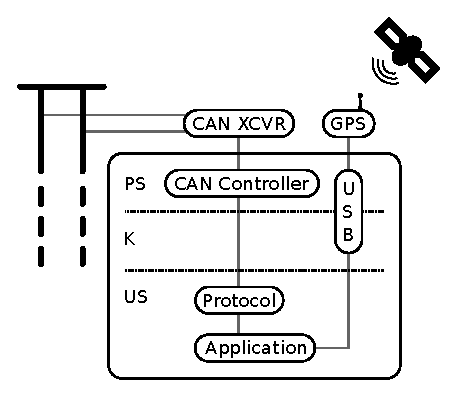
\includegraphics[width=0.5\textwidth]{graphics/analysis_gps.eps}
\caption{GPS node implemented on Zybo board.}
\label{fig:gps_node}
\end{figure}

This specific node has a GPS attached to it connected through a USB interface, but in general it could be any kind of data producing unit connected through any kind of interface.
Because of time constraints the designed software has only been implemented in code to work on a GPS sensor node.
\\From the analysis section it is clear that a sensor node has the following responsibilities:

\begin{itemize}
\item Get data from associated sensor.
\item Pack data according to the specified protocol.
\item Construct and send CAN package.
\item React to the commands it receives.
\end{itemize}

Analyzing on the procedure when data goes from a sensor to the CAN program resulted in the block diagram of figure \ref{fig:filter_1}.

\begin{figure}[!h]
\centering
\begin{subfigure}{0.45\textwidth}
\centering
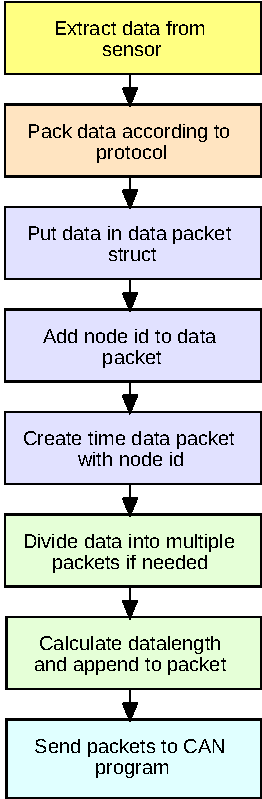
\includegraphics[width=0.60\textwidth]{graphics/FlowChart_Node_Packing}
\caption{Outgoing data. Data going from a sensor and to the CAN program.}
\label{fig:filter_1}
\end{subfigure}
~
\begin{subfigure}{0.45\textwidth}
\centering
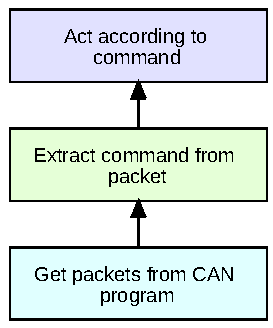
\includegraphics[width=0.60\textwidth]{graphics/FlowChart_Node_Unpacking}
\caption{Ingoing data. Data going from the CAN program to the node.}
\label{fig:filter_2}
\end{subfigure}
\caption{Block diagram showing handling of outgoing and ingoing data. The boxes are colored according to which class implements the functionality. Yellow is the GPS class, orange is the Packer\_GPS class, purple is the node class, green is the protocol class and blue is the CAN\_link class.}
\label{fig:flow_flow}
\end{figure}

To design modular software it needs to be analyzed which blocks are the same for all nodes and which are sensor specific.
The sensor specific tasks are found to be extracting data from sensor and to pack data according to the protocol.
The remaining tasks are the same for all sensor nodes in the system. 
The procedure when data is going from the CAN program to the node is shown in figure \ref{fig:filter_2}.
All tasks are found to be generic for all sensor nodes.

\subsubsection*{Class diagram}
Based on the previous analysis a class diagram was developed and can be seen in figure \ref{fig:node_class_diagram}.
The classes main responsibilities are shown in figure \ref{fig:flow_flow}.
Classes GPS and GPS\_Packer is sensor specific and should be developed for each specific sensor.
In a generic sensor node the GPS class would be a sensor class and the Packer\_GPS class would be a Packer\_Sensor. 
Classes to the left are agnostic to all data they receive going from the sensor and to the CAN network.
They are generic classes and should be reused when developing new nodes.

\begin{figure}[!h]
\centering
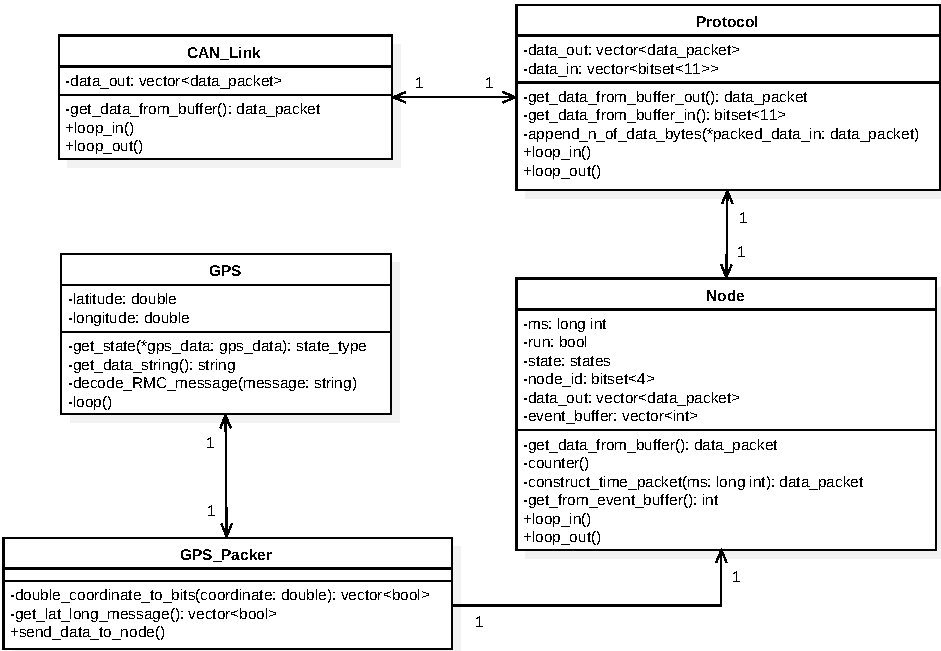
\includegraphics[width=1\textwidth]{graphics/ClassDiagram_NodeSimple}
\caption{Class diagram showing sensor node software.}
\label{fig:node_class_diagram}
\end{figure}

A struct containing all fields of a data packet in boolean data types is defined in listing \ref{code:data_packet}.  

\begin{lstlisting}[caption=Struct for data packet.,label=code:data_packet]
struct data_packet {
  std::bitset<1> nw_msg;
  std::bitset<4> node_id;
  std::bitset<4> dlc;
  std::bitset<6> messagetype;
  std::vector<bool> data; 
  (*@\makebox[\linewidth][c]{$\smash{\vdots}$}@*)
};
\end{lstlisting}
It will be passed between the classes and they will each add their own information. 

The classes and their tasks will be explained here.

~\\ \par \textbf{GPS class} ~ \\
The GPS class needs to extract data from a connected GPS unit and update its own variables with that data.
The specific GPS unit used in this project has a USB interface and uses the NMEA protocol to format data.

~\\ \par \textbf{Packer\_GPS class} ~ \\
The Packer\_GPS class is also sensor specific and is the link between the sensor and the data agnostic node.
It is hard-coded with the message types that the sensor is allowed to send onto the network.
It has the responsibility to pack data according to the developed protocol.
Data in the form of a vector of booleans are then put into the \texttt{data\_packet} struct and passed to the node class.
The reason for making a separate class for the packer and not putting the functionality into the GPS class is that if the specification of the protocol or message types change, only this class needs to be modified.
Similarly, if the GPS module is replaced, the Packer\_GPS class does not need to be altered.

~\\ \par \textbf{Node class} ~ \\
The Node class gets \texttt{data\_packets} from the Packer class and will then prepend its node ID to the message type.
It needs to create a timestamp \texttt{data\_packet} each time data is to be sent.
In order to create the time message the class needs to keep track of milliseconds since receiving the synchronize message.
The class receives start, stop or synchronize events from the protocol class and reacts to those accordingly.

~\\ \par \textbf{Protocol class} ~ \\
The protocol class receives \texttt{data\_packets} from the node class. 
If it receives \texttt{data\_packets} where there are more than eight data bytes it needs to create additional \texttt{data\_packets} and distribute data to them. 
The additional \texttt{data\_packets} must have the same node id and message types, but the new message, nw\_msg, bit should be set to zero..
The class also needs to calculate number of data bytes, \texttt{dl}, to each \texttt{data\_packet}.
On \texttt{data\_packets} coming from the CAN network the class needs to use the last two bits of the messagetype to decode which command is sent to the node.

~\\ \par \textbf{CAN\_link class} ~ \\
The CAN\_link class has the responsibility of transferring and receiving data to and from the CAN program.
As this interface has not yet been implemented this class makes use of the standard input and output. 
Meaning that data from the sensor will be printed in the shell and data to the node should be written to the shell. 

\subsubsection*{Passing data between classes}
Communication between classes is realised by using the producer-consumer pattern.
As the name implies one class produces data and puts this in a queue where another class consumes by taking data out of the queue.
To get the producer and consumer functions to run in parallel they are run in separate threads.
All queues are protected by a mutex to make the software thread-safe.

\subsubsection*{Node class functionality}
The functionalities of the Node class on outgoing data is implemented using a state machine.
It is shown in figure \ref{fig:state_machine}.
\begin{figure}[!h]
\centering
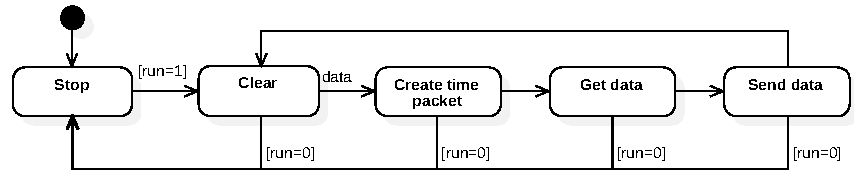
\includegraphics[width=1\textwidth]{graphics/StateDiagram_Node.pdf}
\caption{State machine implementing the node class functionality. }
\label{fig:state_machine}
\end{figure}
\martin{In figure~\ref{fig:state_machine}, the "boolean" value run, should be the same as the boolean value "running" on figure~\ref{fig:node_class_diagram}.}
When the variable \texttt{run} is equal to 1, the node should output sensor data.
\texttt{run} is being updated by the thread that handles incoming commands.
It will then go the clear state and clear all variables and wait for data. 
When data is present it will move through the states create time packet, get data and send data. 
If at any point \texttt{run} is set to 0 the state machine will go to the stop state.
In the stop state the input queue of \texttt{data\_packet} will be cleared.











\subsection{WiFi Node}
The node with a WiFi connection to the stationary computer is a special node in the system.
There should be only one and it should collect all CAN messages, log them and transfer them using WiFi.
Because of time constraints the software designed in this has not been implemented in code.
The WiFi node can be seen in figure \ref{fig:wifi_node}.

\begin{figure}[!h]
\centering
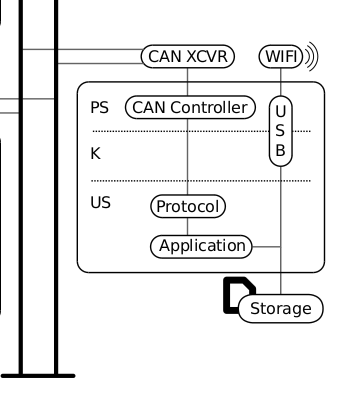
\includegraphics[width=0.4\textwidth]{graphics/wifi_node}
\caption{WiFi node implemented on Zybo board.}
\label{fig:wifi_node}
\end{figure}

From the analysis it is clear that the WiFi node has the following responsibilities:

\begin{itemize}
\item Log all data to SD card.
\item Transmit and receive data through WiFi.
\item Pack data according to protocol.
\item Send log file through WiFi upon request.
\item Timestamp management.
\item Merge multi frame packets.
\end{itemize}
\mikkel{Is multi frame packets what we mean?}
\martin{Yes, I think we mean that. But is timestamp managing a task for the WiFi node?}

It is found that the responsibilities can be grouped into normal operation mode and sending log file mode.
This should be implemented as a state machine as shown in figure \ref{fig:StateDiagram_NodeWiFiStates}.
In normal operation mode the WiFi node should handle data coming from the CAN network and the data coming from the WiFi connection.
If it receives a \texttt{send\_log} command from the stationary computer it should go into the sending log mode and stay there until the log file has been sent.

\begin{figure}[!h]
\centering
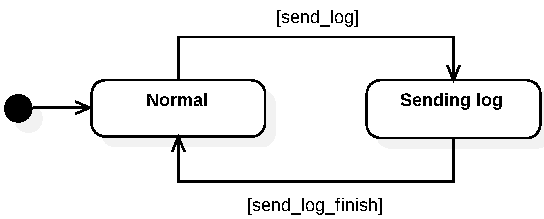
\includegraphics[width=0.5\textwidth]{graphics/StateDiagram_NodeWiFiStates}
\caption{State machine in WiFi node software.}
\label{fig:StateDiagram_NodeWiFiStates}
\end{figure}

In normal operation mode it should handle all incoming data from the WiFi connection as shown in figure \ref{fig:FlowChart_NodeWiFiCmd}.
As it can be seen the WiFi node will only send frames to the CAN network when it receives commands to do so from the stationary computer.

\begin{figure}[!h]
\centering
\begin{subfigure}[b]{0.42\textwidth}
\centering
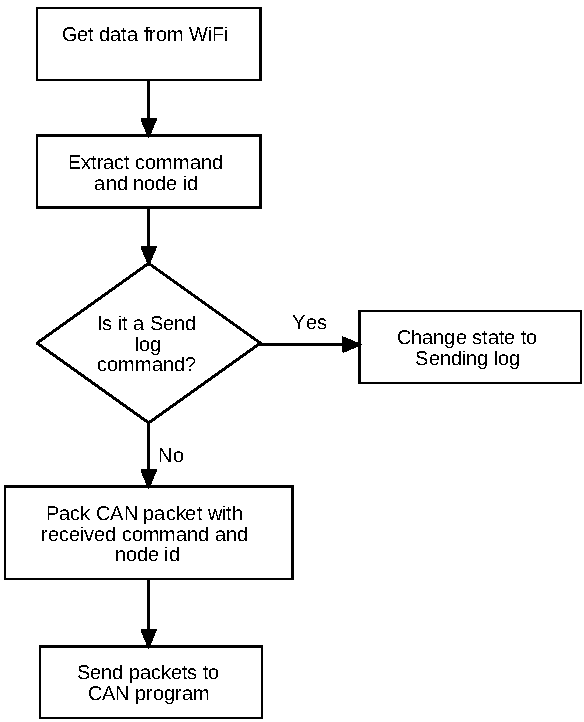
\includegraphics[width=1\textwidth]{graphics/FlowChart_NodeWiFiCmd}
\caption{Handling of data received through WiFi.}
\label{fig:FlowChart_NodeWiFiCmd}
\end{subfigure}
~
\begin{subfigure}[b]{0.52\textwidth}
\centering
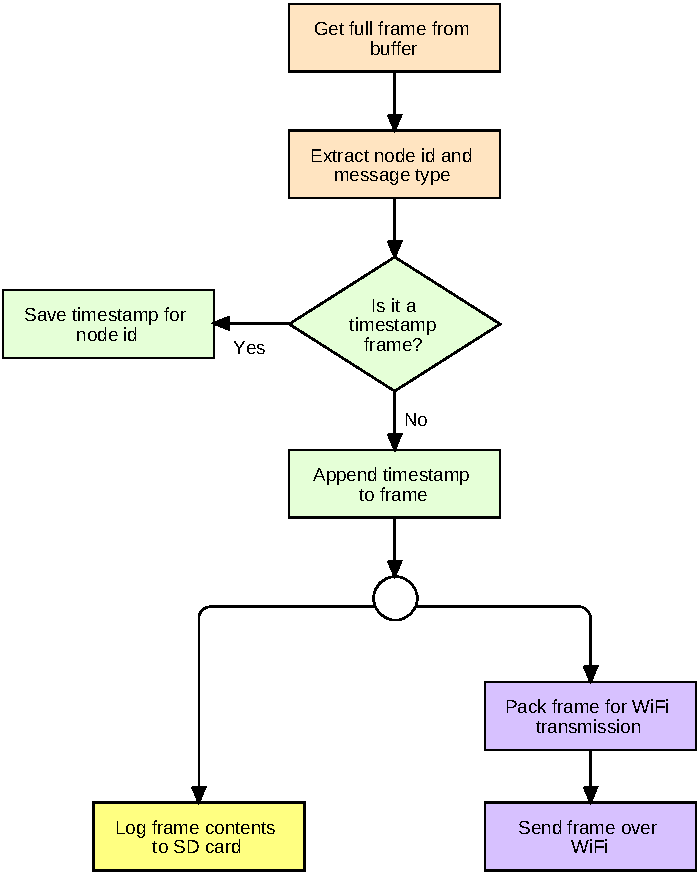
\includegraphics[width=1\textwidth]{graphics/FlowChart_CANFrameProcess}
\caption{Handling of data received from CAN network.}
\label{fig:FlowChart_CANFrameProcess}
\end{subfigure}
\caption{Block diagram showing handling of outgoing and ingoing data. The boxes are colored according to which class implements the functionality. Purple is the WiFi class, pink is the state machine class, orange is the protocol class, green is the CAN\_link class, blue is the timestamper class and yellow is the logger class.}
\label{fig:wifi_flow}
\end{figure}

In normal operation mode the WiFi node needs to receive CAN frames from the CAN program. 
Some frames contain data that is split into more frames.
In order to log and timestamp data correctly these frames needs to be merged together.
The \texttt{new\_msg} field in the messageid will be \texttt{0} if a received frame needs to be merged with the previously received frame.
A state machine handling merging of frames can be seen in figure \ref{fig:StateDiagram_ConcatMsgProcess}.

\begin{figure}[!h]
\centering
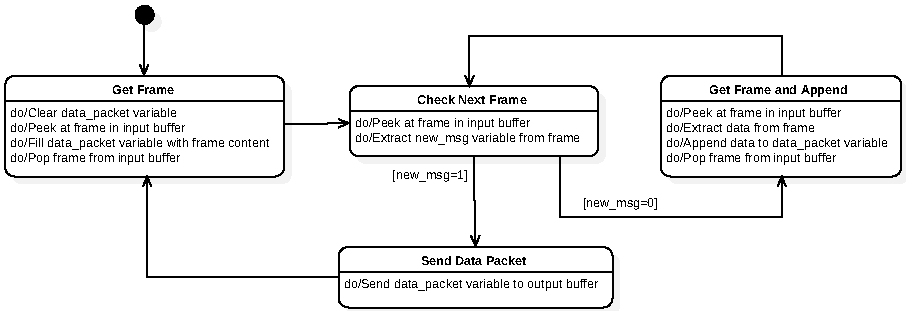
\includegraphics[width=1\textwidth]{graphics/StateDiagram_ConcatMsgProcess}
\caption{Merging multi frame packets together.}
\label{fig:StateDiagram_ConcatMsgProcess}
\end{figure}

The mentioned input buffer is the buffer where the CAN program puts its received frames. 
When the frames are correctly merged they will be put in the merged frame buffer.
The frames in this buffer then needs to be timestamped correctly, logged and sent throug WiFi.
This flow is depicted in figure \ref{fig:FlowChart_CANFrameProcess}.


\subsubsection*{Class diagram}
Based on the previous analysis a class diagram was developed and can be seen in figure \ref{fig:node_class_diagram}.
The classes main responsibilities are shown in figure \ref{fig:wifi_flow}.

\begin{figure}[!h]
\centering
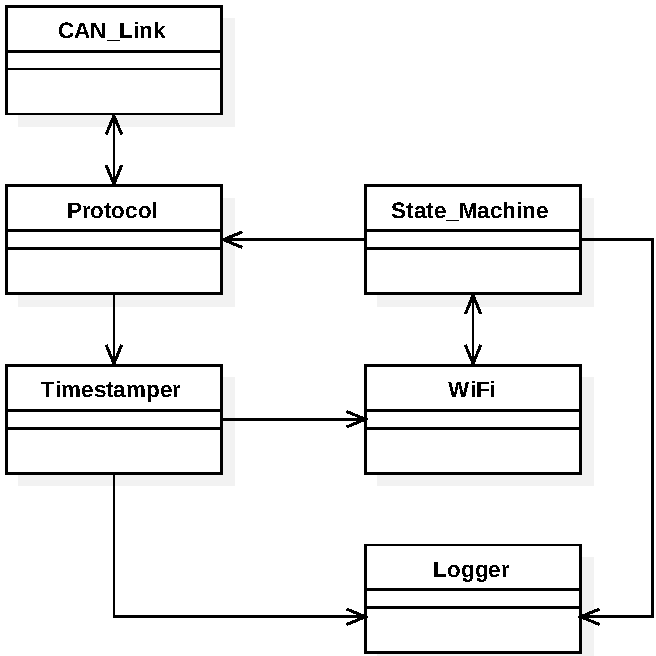
\includegraphics[width=0.6\textwidth]{graphics/ClassDiagram_NodeWiFi}
\caption{Class diagram showing sensor node software.}
\label{fig:StateDiagram_ConcatMsgProcess}
\end{figure}

\mikkel{Should these class descriptions be omitted?}
\subsubsection*{WiFi class}
The WiFi class needs to receive and transmit data through the connected WiFi dongle.
It receives data from the Timestamper class in normal mode and data from State\_Machine in sending log mode.
The State\_Machine also sets if it should transmit the data it gets from the Timestamper class. 

\subsubsection*{State\_Machine class}
The State\_Machine class implements the state machine of figure \ref{fig:StateDiagram_NodeWiFiStates}.
When sending log mode it needs to get a log file from the logger class and give it to the WiFi class.
When i normal mode it needs to extract commands and node ids from the received WiFi data and give it to the Protocol class.

\subsubsection*{Protocol class}
The Protocol class needs to get frames from the full frame buffer and extract node id and messagetype. 
It also needs to pack CAN frames with received commands and node id from the State\_Machine class.

\subsubsection*{CAN\_link class}
The CAN\_link class has the responsibility of transferring and receiving data to
and from the CAN program.

\subsubsection*{Logger class}
The logger class needs to log all received data to a SD-card.
It also needs to read the logged file and transfer it to the State\_Machine classes, when in sending log mode.

\subsubsection*{Timestamper class}
The Timestamper class needs to do the timestamp management described earlier.
It needs to keep the latest received timestamp for each node in the network.
When it receives data from a node it should append the latest received timestamp from that node.  
\section{Sensors}
%!TEX root = ../main.tex
\subsection{Implementation of sensors}\label{sub:implementation_of_sensors}
This section will describe the implementation of the sensors selected during the analysis.
%!TEX root = ../main.tex
%Motor data object: 4600h. includes motor slip frequency (not relevant), currents, voltages and temperature of heatsink. Don't know yet what the subindices are.
%It is possible to map them to Process Data Object for fixed time updates. It doesn't say anywhere what update rate, we can achieve.
%I've gotten a good amount of data from Karsten.

%This section assumes that CANopen has been adequately explained beforehand

\subsection{Interfacing with Sevcon}\label{sub:Sevcon_interfacing}
The Sevcon Gen4, currently on the go-kart, is compatible with CAN.
However, as it is a general purpose motor driver, it cannot be programmed to use GoCAN. 
For this reason, and to make the network unaffected by replacement of the motor driver, it has been decided to use a Zybo to interface with the Sevcon.

\subsubsection*{Physical Connection}\label{sub:sevcon_physical_connection}
Communication with the Sevcon is done through a high speed CAN bus that needs to adhere to ISO11898-2.
As described in section~\ref{sub:CANphys}, one transceiver board has two transceivers along with a terminal so that one Zybo can connect to the Sevcon using the second CAN controller.

\subsubsection*{Sevcon Object Dictionary}\label{sub:sevcon_object_dictionary}
The Sevcon utilizes CAN open, which means all of its parameters are listed in an object dictionary.
Because the Sevcon is a general purpose AC motor driver, its object dictionary is very large, and holds a lot of objects that are irrelevant for this particular setup, such as motor slip, and speed control parameters. 
The object directory is documented in a 1400+ line Excel file. 
Some objects of interest listed in table \ref{tab:parameters_of_interest}.

\begin{table}[h]
	\centering
	\begin{tabular}{| c | c |}
		\hline
		Parameters & Index-subindex \\ % Excel line
		\hline
		Motor Temperature & 4600h-3 \\ % 977
		Measured Id & 4600h-7  \\ %981
		Measured Iq & 4600h-8  \\ %982
		Measured Vd & 4600h-9  \\ %983
		Measured Vq & 4600h-10 \\ %984
		Target Id & 4600h-5    \\ %979
		Target Iq & 4600h-6    \\ %980
		Encoder Read-out & 4630h-9 to 12 \\ %1137
		Throttle value & 2620h \\ %330
		Velocity & 606Ch       \\ %1378
		\hline	
	\end{tabular}
	\caption{List of some of the parameters readable through CANopen}
	\label{tab:parameters_of_interest}
\end{table}

For the most part, these values have 16 bit resolution, which means they can be grouped together four at a time in a process data object.
The fact that a value can be mapped to a PDO means, that it can be transmitted to the Zybo at fixed time intervals or whenever it is updated.
The Encoder Read-out sin/cosine encoder position, so it needs to be converted to mechanical angle. 
This is done using equation~\ref{eq:cos_sin_to_degree}

\begin{equation}
\Omega_m = \mathrm{atan2}(\cos,\sin)
\label{eq:cos_sin_to_degree}
\end{equation}

These adaptations need to be done to make the Sevcon node a generic motor driver node.
That way it would be possible to use this system with a custom made inverter.

\martin{We need to write something about implementation of the other sensors. We also need to use the same order throughout the report}
\section{System Front End}
%!TEX root = ../main.tex
\subsection{\acs{ui} Backend}
\thomas{ensure that they actually do state that this is a requirement}
The requirements state that it should be simple to add additional sensors to the system.
Adding a sensor includes creating a way of easily accessing and showing the data on the observing system.
This section will explain the design of the backend that will provide this functionality.

\subsubsection*{Data Format}
Depending on the author of the data (which node produced the data) the data may be inherently different.
The interpretation of data is therefore not uniform across the entire system.
For this reason, it is necessary to create a system that is agnostic with respect to the type and amount of data being handled.
In section \ref{sub:CAN_protocol} a description of the node and message identification system is given.
The NodeID and MSGtype identifiers are decided by the implementer and together they provide a unique, 11 bit identifier, the Message ID, for the type of data in the message.
Since the Message ID is capable of uniquely identifying the data, it will be used in storing the data.
Additionally each message will be associated with a four byte timestamp.
This timestamp is given as the time in milliseconds since startup and is associated with message type <type>. \thomas{insert correct message type}
\thomas{We need to agree on a way to write nodeid,msgid,msgtype throughout the report}

\subsubsection*{Backend Architecture}
An overview of the functionality can be seen in figure \ref{fig:backendconcept}.
As can be seen, this architecture provides the link between the receiving program (socat) and a potential \acs{gui}.
Upon receiving a message from the go-kart, socat will pipe the raw message to the interpreter.
The interpreter will proceed to extract the message id, the timestamp and the data.
These are then put into a fifo buffer which will contain the latest 1024 data points for a given message id.
\thomas{Why 1024? An arbitrary number that needs some sort of explanation..}
The backend is a collection of functions which provide an API for the UI layer. 

\begin{figure}
	\includegraphics[width=\linewidth]{graphics/backend_concept}
	\caption[Overview of the backend functionality.]{Overview of the backend functionality. 
	Messages are received over wifi from the go-kart. 
	An interpreter reads the message to determine the MessageID (MSGID), timestamp (T) and the data. 
	All information is made available to a \acs{gui} through the backend.}
	\label{fig:backendconcept}
\end{figure}

\begin{figure}[H]
	\missingfigure{Backend Class Diagram}
	%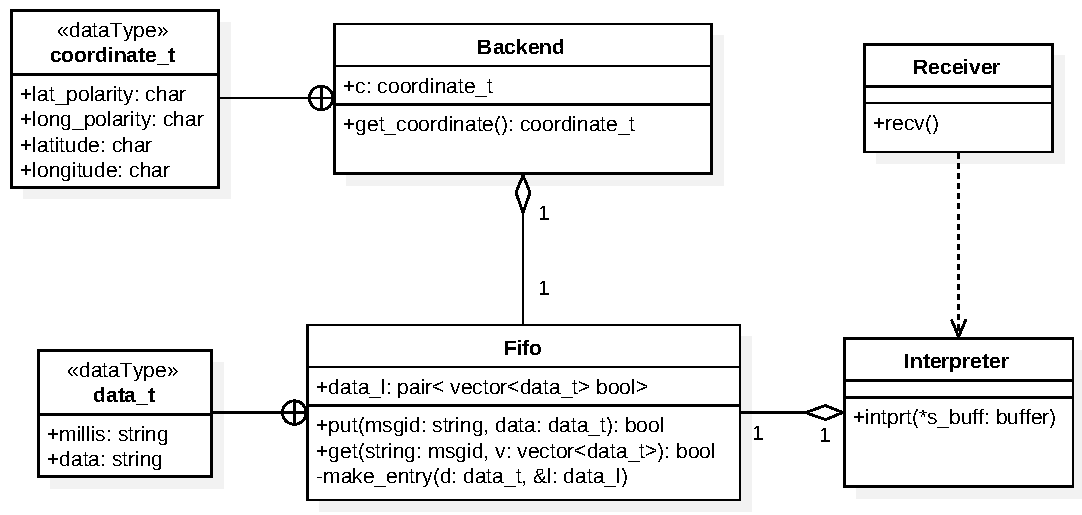
\includegraphics[width=\linewidth]{graphics/backend_class_diagram}
	\caption[Backend class diagram.]{Classdiagram of the backend.}
	\label{fig:backendclass}
\end{figure}

From \ref{fig:backendconcept}, a class diagram has been created.
This can be seen on figure \ref{fig:backendclass}.
Four classes are created, each of which will be explained in more detail below

\paragraph*{\texttt{receiver}}~\\
This class is run in a separate thread.
It continuously listens to std::io, waiting for input from the go-kart.
Upon receiving a message, it is put into a buffer maintained by interpreter.
\paragraph*{\texttt{interpreter}}~\\
As mentioned, this class holds a message buffer, shown in code \ref{code:msgbuffer}.
Whenever a message is put in the buffer, it is split into its three components, a 10 bit message id, a 4 byte timestamp and an data of arbitrary length.
On figure \ref{fig:backendmsg} is a depiction of a message.
\begin{figure}[H]
	\missingfigure{Backend Message (msgid/timestamp/data)}
	%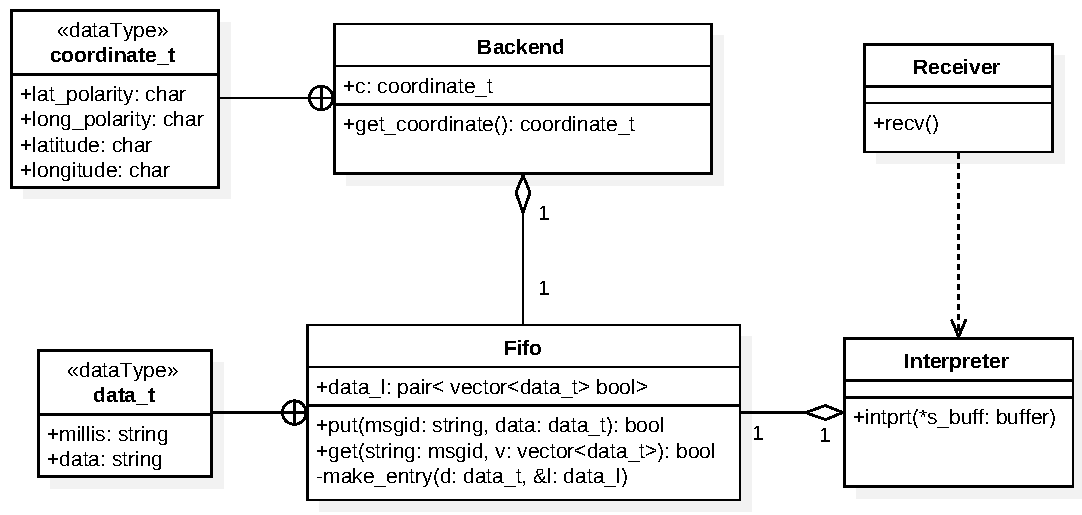
\includegraphics[width=\linewidth]{graphics/backend_class_diagram}
	\caption[Wifi Message.]{Depiction of the message sent over wifi.}
	\label{fig:backendmsg}
\end{figure}

Once split, the information is stored using the put function 
\begin{lstlisting}[caption=Buffer for holding incomming messages,label=code:msgbuffer]
struct buffer 
{
  std::vector<std::string> strings;
  std::mutex mutex;
};
\end{lstlisting}
\newpage
\part{Verification}
%!TEX root = ../main.tex

\thomas{We need to find a good naming convention for these sections - having "tests" in the headline doesn't quite sound right..}
Throughout this section tests will be designed and carried out in order to verify that the various subsystems live up to the requirements set in section \ref{sec:system_requirements}.\\

%\subsubsection{Utilizing Service Virtualization for the Proof of Concept}
\label{sub:Utilizing_Svr_Virtualization}
\catalin{More details here after a group discussion and opinions.}
\martin{I moved this here, at it really is a desription of how we test the system from several angles}
In order to show that the system can be fully functional despite the unsuccessful attempt to implement it, a different approach than the actual implementation is needed.
One way of doing that is to apply a method called service virtualization where one part of the system can be simulated to prove that the rest of the system is fully functional, given the presence of the missing simulated part.
\\
In this case, the system that was designed for this project can be divided into two parts or subsystems.
The first one is the physical CAN network to this point is only functional in bare\-metal code, which is described in section~\ref{sub:CAN_Bus_Tests}.
The second part would be considered the subsystem present on Linux which included the protocol designed to be used with the CAN bus and the application which extracted the data from the sensors.
This is described in section~\ref{sec:node_software}
The connection between the two subsystems is the service virtualization and could be replaced either by a software buffer.

%!TEX root = ../main.tex

\section{CAN Bus}
\label{sub:CAN_Bus_Tests}
With the CAN controller available on the PS of the Zybo, the CAN bus will be tested to determine the transmission capabilities of the network.
The transceivers are able to work at up to 8 Mb/s, while the CAN controllers on the Zybo only guarantee functionality up to 1 Mb/s. \\

The tests are performed using the design from figure~\ref{fig:CAN_Testing_Architecture}, on page~\pageref{fig:CAN_Testing_Architecture} as the FPGA part, though not all parts of this design is used for each test.
Software was developed for bare-metal purpose, and because of this, not all tests were performed using interrupts, as the Zybo had no other task that it could be interrupted from.

The tests performed will be: 
\begin{itemize}
	\item \textbf{Basic communication}: verifying the ability for basic communication between nodes, while confirming, that the CAN stack works.
	\item \textbf{Latency tests}: Measuring the time it takes to send one full frame.
	\item \textbf{Bandwidth}: Determining how much raw data can be transmitted per unit time.
	\item \textbf{Priority when multiple node sending}: Ensuring, that higher message ID make way for the lower ones.
\end{itemize}

\subsection{Basic Communication}
\label{sub:TestingCANStack_BareMetal}


\mikkel{Changed!}
In order to verify that the basic communication of a CAN network works on the developed CAN bus a test needs to be conducted.
The method of the test was to implement the functionality of sending the input value of a pressed button to the network and to receive frames from the network, decode the frames and turn on the appropriate LED.
The flow of event for sending a frame is shown in figure \ref{fig:FlowChart_CANSoft_BtnsIntr} and the flow for the receiving a frame is shown in figure \ref{fig:FlowChart_CANSoft_RecvData}.

\begin{figure}[h!]
	\centering
	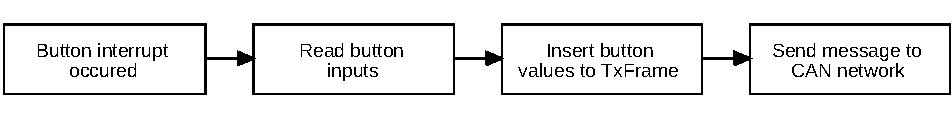
\includegraphics[width = 1\linewidth]{graphics/FlowChart_CANSoft_BtnsIntr.pdf}
	\caption{Flow chart with button interrupts.}
	\label{fig:FlowChart_CANSoft_BtnsIntr}
\end{figure}

\begin{figure}[h!]
	\centering
	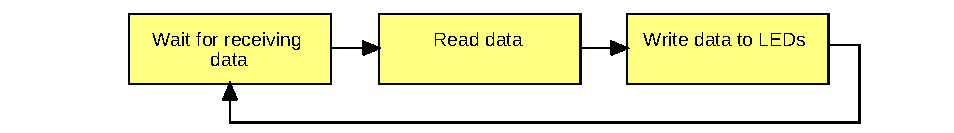
\includegraphics[width = 1\linewidth]{graphics/FlowChart_CANSoft_RecvData.pdf}
	\caption{Flow chart for the process of receiving data.}
	\label{fig:FlowChart_CANSoft_RecvData}
\end{figure}


All Zybos involved in the test was programmed with the architecture shown in figure \ref{fig:CAN_Testing_Architecture} and programmed with both the functionality of sending and receiving frames.
\\~\\
When pressing a button on a Zybo the appropriate LED on the other LED turned on, verifying that frames were packed, transmitted, received and unpacked correctly. 
The test was also performed with multiple Zybos connected to the CAN bus, in this case pressing a button on a Zybo turned on the appropriate LEDs on the rest of the Zybos.


%% THIS IS NOT USED ANYWHERE AND THEREFORE OMITTED
% \paragraph*{Runtime with GPIO Interrupts}~\\
% The software's behavior is similar in this case, as well as it can be seen in figure \ref{fig:FlowChart_CANSoft_GPIOIntr}.
% The difference is that instead of button values, dummy data may be inserted into the TxFrame according to the simulation needs and the receiving data is only presented in the SDK terminal.
% \begin{figure}[h!]
% 	\centering
% 	
\includegraphics[width = 1\linewidth]{graphics/FlowChart_CANSoft_GPIOIntr.pdf}
% 	\caption{Flow chart with GPIO interrupts.}
% 	\label{fig:FlowChart_CANSoft_GPIOIntr}
% \end{figure}

\subsection{Latency Test}\label{sub:CAN_latency}
For this test, only two Zybos are needed.
One node prepares a frame for transmission, then sets a GPIO pin high.
It then performs the necessary checks and writes the message details to the TX FIFO, and then sets its GPIO pin low. \\

The other node will then wait for the full message frame to be received, and then set its GPIO pin high.
Once the metadata of the message (data length and message ID) has been intepreted, the GPIO pin goes low again.
Using an oscilloscope, it is possible to measure the time it takes to transfer a message.\\

The test will be performed for an 8 byte frame.
The messages will be constructed, so that bit stuffing doesn't occur by writing 0xA1 to 0xA8. 
The resulting voltage measurements are displayed in figure~\ref{fig:CAN_test1_raw}.\\

\begin{figure}[h]
	\centering
	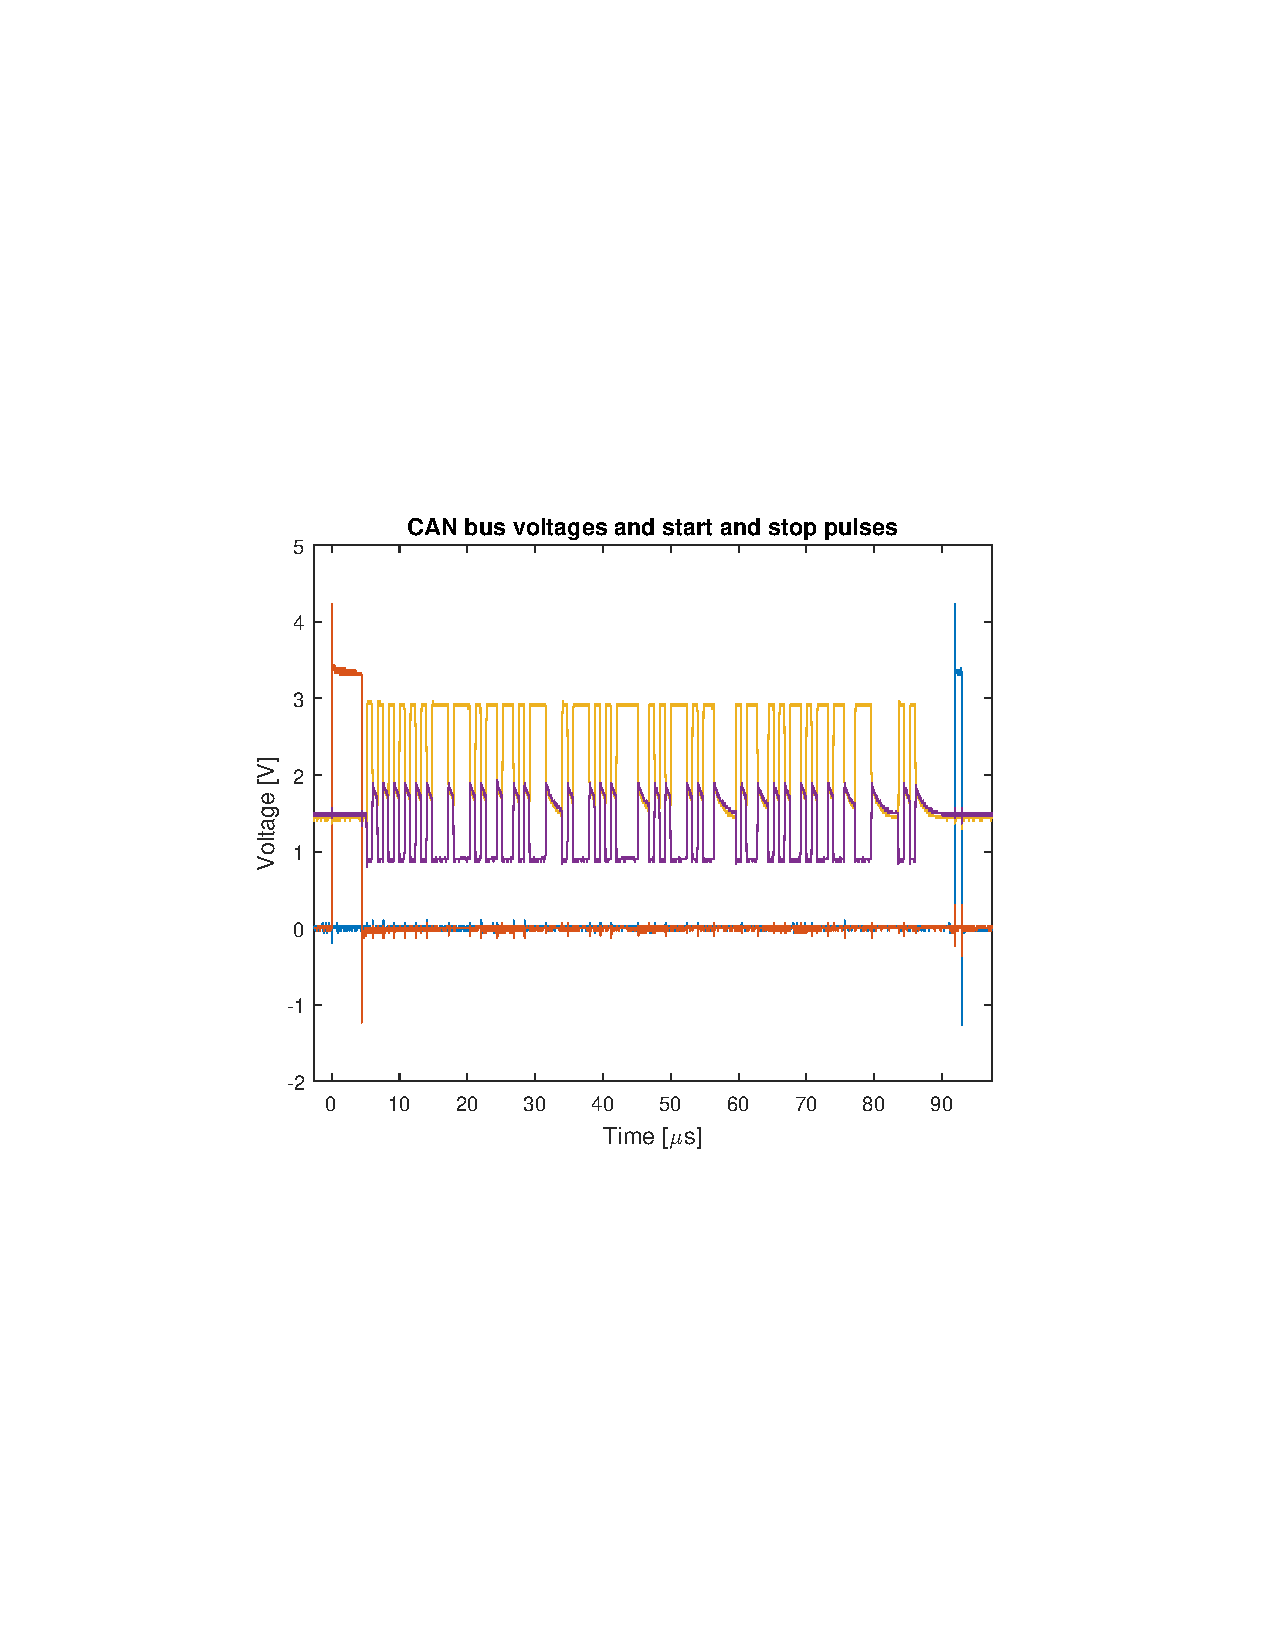
\includegraphics[width = \linewidth]{graphics/CAN_test1_raw}
	\caption[Start and stop pulses for an 8 byte CAN message.]{Start and stop pulses for an 8 byte CAN message. Yellow indicates the voltage of the CAN\_H, purple indicates the voltage of CAN\_L}
	\label{fig:CAN_test1_raw}
\end{figure}

The time from the red voltage goes low, to the time the blue voltage goes high is $87.5 \si{\micro\second}$.
This is of course very dependent on the particular controller used for this test, which according to the datasheet can work up to 1 MHz.
Measuring this test shows, that bit come at 1.25 MHz.
The software used for basis of this test does allow to adjust a pre-scaler, so that the controller works faster, but it is not able to receive frames at a higher rate than 1.25 MHz.\\

The CAN bus voltage can be interpreted to bits, to show what's actually being transmitted.
This is done by measuring the voltage difference between the yellow and purple graphs, keeping in mind, that a difference in voltage corresponds to a zero, while no difference corresponds to a one.
The CAN frame is displayed and interpreted in figure~\ref{fig:CAN_test1_message}.\\

\begin{figure}[h]
	\centering
	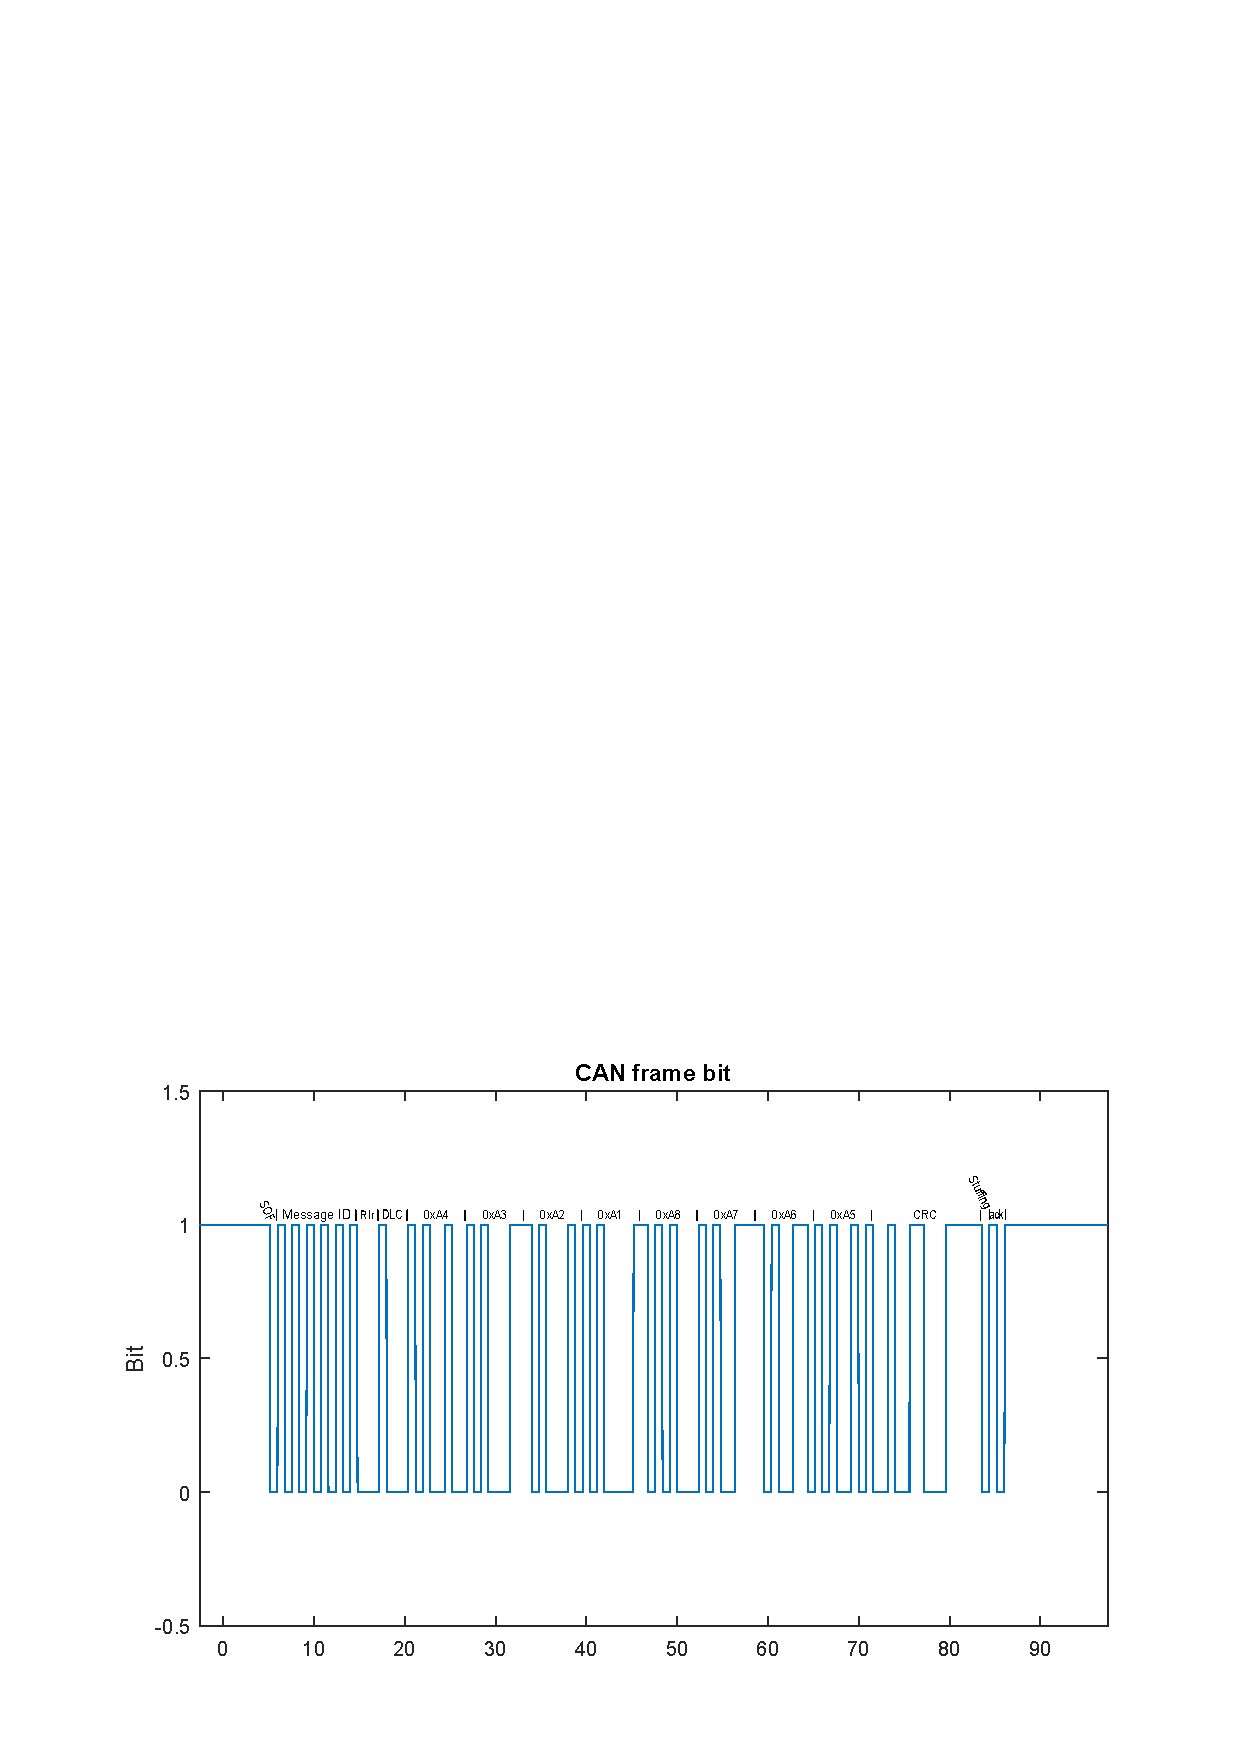
\includegraphics[width = \linewidth]{graphics/CAN_test1_message}
	\caption[Bit interpretation of the CAN frame.]{Bit interpretation of the CAN frame. RIr  is the tree bits: RTR, ID Extention and r0, which are all 0.}
	\label{fig:CAN_test1_message}
\end{figure}

The data portion of the frame is bitwise big endian, but bytewise little endian. 
The message to be sent was codes as two 32 bit unsigned integers: 0xA1A2A3A4 and 0xA5A6A7A8.
The controller then swapped the bytes around, causing the data to become little endian.
This is a convention implemented by the CAN controller, and as the same endianness is applied when sending and receiving the frame, it is irrelevant. 
The message was received correctly.\\

The CRC is calculated automatically by the controller.
Unfortunately it ends on five consecutive \texttt{1}'s, meaning that a \texttt{0} must be stuffed in-between the delimiter, causing the frame to be one bit longer.\\

Additionally this controller uses 5 bits for the IFS part of the frame, rather than the mandatory minimum of 3 bits. 

\subsection{Bandwidth}\label{sub:CAN_bandwidth}
This will be calculated, as the faster controllers are not available.
Bandwidth is considering the amount of net data being transmitted per unit time, when excluding the overhead.
Bandwidth will be calculated for 8 byte frames, and bit stuffing will be omitted.\\

The maximum operating data rate for the transceivers is 8 Mb/s.
As mentioned in section~\ref{sub:CanMessageFrame}, the CAN frame has 47 bits of overhead. 
Including 8 bytes of data, this comes up to 111 bits. 
Time per frame is:

\begin{equation}
\frac{111}{8 \cdot 10^6} = 1.39 \cdot 10^{-5}
\end{equation}

As each frame contains 8 bytes of data, the data rate becomes:

\begin{equation}
\frac{8}{1.39 \cdot 10^-5}= 5.77 \cdot 10^5
\end{equation}

That means, that the effective transfer rate is 577 kB/s, or 4.61 Mb/s with 8 Mb/s controllers. 
With the controllers built into the PS of the Zybo, this effective rate comes down to 720 kb/s.
\martin{Rewrite, so that we do not mention 8 Mb/s here, move that to the future work. Maybe also mention here, that it give up to 4.6 Mb/s}

\subsection{Message Priority}\label{sub:CAN_message priority}
This test is based on the CAN polled example, where two Zybos will transmit data.
The two transmitting Zybos will prepare a CAN frame with the same data content, but different message IDs.
\begin{itemize}
	\item Zybo A will send message ID 0b10100100000.
	\item Zybo B will send massage ID 0b10101000000.
\end{itemize}
I.e. only the fifth and sixth bits have been swapped, meaning that Zybo A will have the higher priority.
Both of these Zybos will prepare their respective Tx frame, and continuously poll the PMOD port.
The PMOD connection must be configured to have pull down, to ensure that unconnected pins are set low.
Using a DC voltage source, the GPIO port of each Zybo will be set high simultaneously.\\

When the PMOD returns a non-zero value, each Zybo will call the XCanPs\_Send function twice.
This will fill two frames with 8 bytes of data into the Tx FIFO of each Zybo. 
Because of the asynchronous nature of the CAN protocol, it is still somewhat random which message gets transmitted first, so the frame will be sent twice. 
This means, that after the first frame is sent from either one of the Zybos, both zybos will start transmitting at the same time. 
In this case one Zybo must stop transmitting when it detects, that it has the lower priority.
This is shown in figure~\ref{fig:CAN_test3_2TX}.\\

\begin{figure}[h]
	\centering
	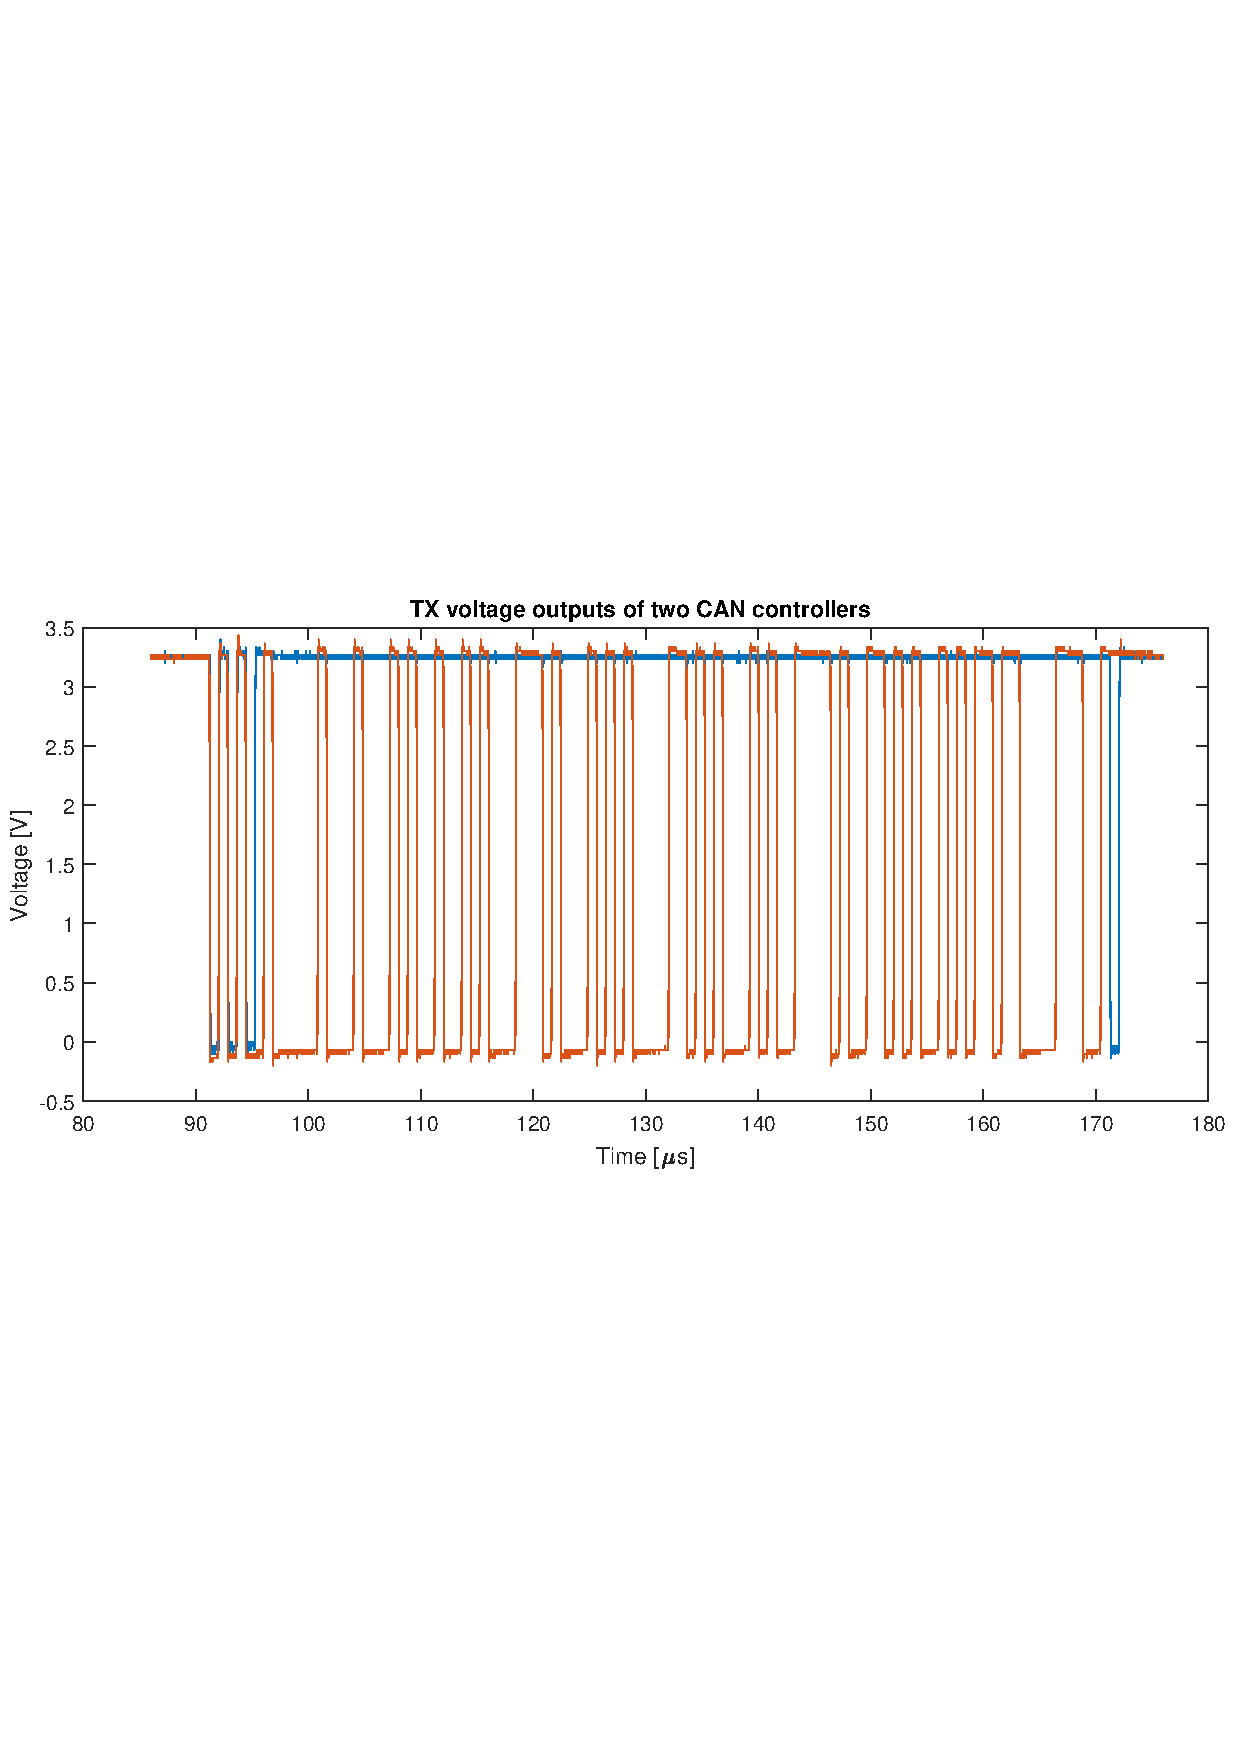
\includegraphics[width = \linewidth]{graphics/CAN_test3_2TX}
	\caption[Voltage measurements of CAN test.]{Voltage measurements taken at the TX pin of Zybo A (red) and Zybo B (blue).}
	\label{fig:CAN_test3_2TX}
\end{figure}

The displayed frame is the second of four frames sent for this test, which is why the graph starts at $80 \si{\micro\second}$.
Both Zybos start sending their frame simultaneously, and as there is no difference until the fifth bit of the message ID, neither Zybo is aware that the other is also sending.
At the time $95\si{\micro\second}$, Zybo B (blue line in figure~\ref{fig:CAN_test3_2TX}) sends out high, whilst receiving low, meaning that another node is sending as well. 
It will then cancel this attempt to transmit, and wait until the current frame has been transmitted before it will try again.
Also note the Zybo B writing the acknowledge bit at the time $171 \si{\micro\second}$.
Because of this, it is not strictly necessary to use a receiving Zybo, because the other node will confirm the CRC of the message.\\

\subsection{Conclusion}\label{sub:CAN_test_conclusion}
It has been shown that the CAN hardware does work.
It is possible to transmit a message from one Zybo to another, without error.
The substantial overhead does limit the potential data bandwidth.
Additionally it was possible to measure the time it takes to construct a CAN frame, although this might vary a great deal from one controller to the next.

\begin{table}[h!]
	\centering
	\begin{tabular}{r | c | c}
		\textbf{Parameter} & \textbf{xcanps controller} & \textbf{8 Mb/s CAN controller} \\
		\hline
		\textbf{Frame time} & $87.5 \si{\micro\second}$ & $13.7\si{\micro\second}$ \\
		\textbf{Build time} & $4.43 \si{\micro\second}$ & - \\
		\textbf{Data bandwidth} & $720 \mathrm{kb/s}$ & $4.61 \mathrm{Mb/s}$
	\end{tabular}
	\caption{Results obtained from the test of the CAN bus.}
	\label{tab:CAN_test_conclusion}
\end{table}

%!TEX root = ../main.tex
\subsection{Wifi}
This section 
%!TEX root = ../main.tex
\section{Node Software}
\label{sec:node_software}
When addressing the node software it is important to remember the distinction between sensor node software and wifi node software.
The software for the wifi node has not yet been fully implemented therefore this section will only address the verification of the functionalities of the sensor node software implemented on a GPS sensor node.

\subsection{GPS Sensor Node}
The functionality of the developed GPS sensor node software was tested as shown in figure \ref{fig:sensor_gps_veri}.
The GPS service virtualization was run to input data as a GPS module does. 
The GPS node software then processed the data and output it to standard output as the CAN bus connection was not realized.

\begin{figure}[h]
	\centering
	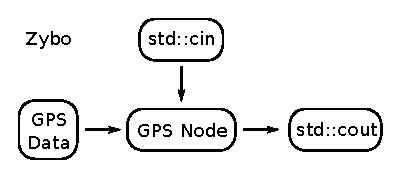
\includegraphics[width = 0.6\linewidth]{graphics/sensor_gps_veri}
	\caption{A line of text}
	\label{fig:sensor_gps_veri}
\end{figure}

When running the software is run it outputs only a string of booleans. 
This is not very readable by humans, so to show the functionality the program was set to print in a humanly understandable way.
A segment of the output from this can be seen in code snippet \ref{code:output_node}.
The first frame should be a timestamp frame. accordingly
It can be seen that the the first frame has node ID 14, 4 data bytes, messagetype 1 and data 2374, meaning that it is from the GPS node with a timestamp of 2374 milliseconds.
The next frame should then be a data frame containing latitude and longitude information.
It can be seen that it has node ID 14, 8 data bytes and messagetype 9, which is a latitude longitude message.
To extract the latitude and longitude from the data field a unpacking algorithm is needed.
Using that it is found that latitude is 55.3673346 degrees North and longitude is 10.4318456 degrees East.

%\begin{lstlisting}[caption=Struct for data packet.,label=code:output_node]
\begin{lstlisting}[language=bash]
(*@\makebox[\linewidth][c]{$\smash{\vdots}$}@*)
Start of frame: 1
Node id: 1110
Number of data bytes: 0100
Messagetype: 000001
Data: 00000000000000000000100101000110
Full frame: 11110000001010000000000000000000000100101000110


Start of frame: 1
Node id: 1110
Number of data bytes: 1000
Messagetype: 001001
Data: 00100001000000000110001010000010000001100011011111000101 11111000
Full frame: 11110001001100000100001000000000110001010000010000 00110001101111100010111111000
(*@\makebox[\linewidth][c]{$\smash{\vdots}$}@*)
\end{lstlisting}

It should be possible to send a sync command to the node by giving it the message ID \texttt{10001111000}.
When typing this into the shell it can be seen that the nodes timestamp is reset.
By sending the message ID \texttt{10001111010} the node stops outputting data.
The node starts sending data again if the message ID \texttt{10001111001} is sent.


\subsubsection*{Conclusion}
The link to the CAN program is not made and therefore the tests are made with standard I/O.
\mikkel{Should there be a conclusion? MAybe it should be omitted?}
By using service virtualization it is verified that the GPS sensor node software has implemented the wanted functionalities.
\mikkel{It should be tested with the real GPS, but this has been omitted because of time constraints?}

%!TEX root = ../main.tex

\section{Front End}
\label{sec:frontendverification}
According to the use cases a user should be able to monitor data created on the network.
This section describes the test done to verify that this functionality is implemented correctly.
\subsection{Method}
Figure \ref{fig:frontendsetup} depicts an overview of the setup used in the verification.
An amount of GPS data is recorded and is presented to the GPS node using service virtualisation.\\

The two parts, CAN-bus and WiFi node were not finished, see sections \ref{sec:methods_to_implement_can} and \ref{sec:somewifinodesection} respectively, as such it was necessary to create service virtualisation for this link.
A small utility was written to serve this purpose, it virtualises the dotted boxes seen in figure \ref{fig:frontendsetup}.
This utility reads the messages sent by the GPS node, extracts the timestamp and inserts it into the data frame in place in the DLC nibble and then outputs it to stdio.
The message is then on the form seen in figure \ref{fig:backendmsg}, the form expected by the front end.
This means that, seen from the perspective of the front end the underlying structure is correct.

\begin{figure}
	\centering
	\includegraphics[width=.75\linewidth]{graphics/frontend_verification}
	\caption[The setup used to verify the functionality of the front end.]{The setup used to verify the functionality of the front end. 
	The dotted boxes are virtualised but the correct connection is maintained between the Zybo and the PC.}
	\label{fig:frontendsetup}
\end{figure}

In order to most accurately reproduce the actual function of the system, the test was done using a wireless connection between a Zybo and a PC.
The connection was established using the method described in section \ref{sec:wifi}.
On the PC, the front end was started, taking its input from a socat listener.
\begin{lstlisting}
>> ./frontend | socat - tcp-listen:2049
\end{lstlisting}
Then, on the Zybo, the GPS and WiFi nodes were started, piping their output to socat:
\begin{lstlisting}
>> ./sensornode | ./verification | socat - tcp:196.178.10.10:2049
\end{lstlisting}
Here, the first and last data points from the data set are shown:
\begin{lstlisting}
>> N 55.36734 E 10.43185
>> N 55.36707 E 10.43109
\end{lstlisting}
This corresponds with the data created on the GPS node.


\newpage
\part{Postface}
%!TEX root = ../main.tex
\begin{thebibliography}{11} %This number should be higher than the number of entries in the bibliography because reasons...
%	\bibitem{id}
%		Author(s) Last name, First name, Company/Organisation, Year. Full Title
	\bibitem{xcanps}
			https://github.com/Xilinx/embeddedsw/blob/master/XilinxProcessorIPLib/drivers/canps/examples/xcanps\_polled\_example.c
	\bibitem{formulastudent}
			University of Southern Denmark, 2014, http://www.sdu-vikings.dk/
	\bibitem{ath9k}
			Open source, June 2015, https://wireless.wiki.kernel.org/en/users/drivers/ath9k\_htc/devices
	\bibitem{boostchat}
			www.boost.org, Boost C++ Libraries, http://www.boost.org/doc/libs/1\_62\_0/doc/html/boost\_asio/examples/cpp11\_examples.html
	\bibitem{beej}
			Hall, Brian, June 2016, Beej's Guide to Network Programming - Using Internet Sockets.
	\bibitem{CAN_introduction}
			Corrigan, Steve, Texas Instruments, July 2008, Introduction to the Controller Area Network (CAN).
	\bibitem{3.3V_CAN}
			Blackman, Jason and Monroe, Scott, Texas Instruments, January 2013, Overview of 3.3V CAN (Controller Area Network) Transceivers.
	\bibitem{interfacenaming}
			Open source, Nov 2015, Predictable Network Interface Names (https://www.freedesktop.org/wiki/Software/systemd/PredictableNetworkInterfaceNames/)
	\bibitem{xillinux}
			Xillybus LTD, http://xillybus.com/xillinux
	\bibitem{Xilinx_wiki_amp}
			Xilinx wiki Asymmetric Multiprocessing, http://www.wiki.xilinx.com/Multi-OS+Support+(AMP+\%26+Hypervisor)
	\bibitem{Xilinx_wiki_Linux_CAN_driver}
			http://www.wiki.xilinx.com/Linux+CAN+driver
	\bibitem{CANopen_introduction}
			http://www.ni.com/white-paper/14162/en/
	\bibitem{Xilinx_AMP}
			John McDougall, February 14, 2013, XAPP1078 v1.0, Simple AMP Running Linux and Bare-Metal System on Both Zynq SoC Processors, https://www.xilinx.com/support/documentation/application\_notes/xapp1078-amp-linux-bare-metal.pdf
	\bibitem{CAN-Utils}
			CAN-Utils tool, https://github.com/linux-can/can-utils/blob/master/README.md
	\bibitem{vectornav}
			VectorNav, vn-100 library, http://www.vectornav.com/support/downloads
	\bibitem{bluetooth}
			Wikipedia, Bluetooth, https://en.wikipedia.org/wiki/Bluetooth
	\bibitem{wiki_wifi}
			Wikipedia, IEEE\_802.11 , https://en.wikipedia.org/wiki/IEEE\_802.11\#Protocol
\end{thebibliography}
\martin{Check cites, ensure that they adhere to the thing and such}
\appendix
%!TEX root = ../main.tex
\newpage
%!TEX root = ../main.tex
\section{Use Case Narratives}
\label{app:usecase}

\begin{table}[H]
\centering
\caption{Usecase narrative for monitor live data from go-kart.}
\label{tab:use_monitor}
\begin{tabular}{| r | p{7 cm} |}
\hline
\textbf{Use case:}                        & Monitor live data                  \\ 
\textbf{Actors:}                          & User                                        \\
\textbf{Purpose:}                         & Monitor live data from go-kart while driving    \\
\textbf{Overview:}                        & The engineer starts the system. The system will begin collecting data on the go-kart and transfer them to a stationary computer. The computer will present data to the engineer on a UI. \\
\textbf{Type:}                            & Essential                                       \\
\textbf{Preconditions:}                   & Go-kart microcontroller is paired with stationary computer                                    \\
\textbf{Postconditions:}                  & System transfers data from go-kart sensors to a stationary computer, showing data in a UI.                                                                                            \\
\textbf{Special requirements:}            & -                                               \\ \hline 
\multicolumn{1}{|c|}{\textbf{Actor action}} & \multicolumn{1}{c|}{\textbf{System response}}\\
\multicolumn{1}{|p{5 cm}|}{1. Start system}       & \begin{tabular}[c]{@{}l@{}}2. Start collecting data\\ 3. Transfer data to stationary computer\\ 4. Present data in UI\end{tabular}                                              \\ \hline
\multicolumn{2}{|c|}{\textbf{Alternative flow of events}}                                   \\
\multicolumn{2}{|p{12 cm}|}{Any line: User can stop the system at any point in time.}              \\ \hline                                                                                                                                    
\end{tabular}
\end{table}


\begin{table}[H]
\centering
\caption{Usecase narrative for log go-kart data.}
\label{tab:use_log}
\begin{tabular}{| r | p{7 cm} |}
\hline
\textbf{Use case:}                        & Log data            			        \\ 
\textbf{Actors:}                          & User                                        \\
\textbf{Purpose:}                         & Log go-kart data                 				\\
\textbf{Overview:}                        & After startup the system will log the collected data locally on the go-kart  \\
\textbf{Type:}                            & Essential                                       \\
\textbf{Preconditions:}                   & System is running and collecting go-kart data   \\
\textbf{Postconditions:}                  & System logs collected go-kart data.      		\\
\textbf{Special requirements:}            & -                                               \\ \hline 
\multicolumn{1}{|c|}{\textbf{Actor action}} & \multicolumn{1}{c|}{\textbf{System response}} \\
\multicolumn{1}{|p{5 cm}|}{}       & \begin{tabular}[c]{@{}l@{}}1. Log collected data locally on go-kart\end{tabular}\\ \hline
\multicolumn{2}{|c|}{\textbf{Alternative flow of events}}                                   \\
\multicolumn{2}{|p{12 cm}|}{Any line: User can stop the logging	at any point in time.}         \\ \hline                                                                                                                                    
\end{tabular}
\end{table}



\begin{table}[H]
\centering
\caption{Usecase narrative for read logged data.}
\label{tab:use_read_log}
\begin{tabular}{| r | p{7 cm} |}
\hline
\textbf{Use case:}                        & Read logged data  			                    \\ 
\textbf{Actors:}                          & User                                        \\
\textbf{Purpose:}                         & To read data that is logged locally on the go-kart               \\
\textbf{Overview:}                        & The engineer will ask the system for the logged data. The system will transfer the logged data to a stationary computer \\
\textbf{Type:}                            & Essential                                       \\
\textbf{Preconditions:}                   & Data is logged in logfile on the go-kart                \\
\textbf{Postconditions:}                  & The log file is on the stationary computer                                                                                      \\
\textbf{Special requirements:}            & -                                               \\ \hline 
\multicolumn{1}{|c|}{\textbf{Actor action}} & \multicolumn{1}{c|}{\textbf{System response}}\\
\multicolumn{1}{|p{5 cm}|}{1. Ask for log file}       & \begin{tabular}[c]{@{}l@{}}2. Transfer logged data to stationary computer\\ 3. Save data to log file on stationary computer\end{tabular}                                              \\ \hline
\multicolumn{2}{|c|}{\textbf{Alternative flow of events}}                                   \\
\multicolumn{2}{|p{12 cm}|}{Any line: If connection is lost the system should detect it and mark the trasferred log file as invalid}              \\ \hline                                                                                                                                    
\end{tabular}
\end{table}

\begin{table}[H]
\centering
\caption{Usecase narrative for start and stop data collection.}
\label{tab:use_start_stop}
\begin{tabular}{| r | p{7 cm} |}
\hline
\textbf{Use case:}                        & Toggle data collection  			                    \\ 
\textbf{Actors:}                          & User                                        \\
\textbf{Purpose:}                         & To start and stop data collection from specified sensors              \\
\textbf{Overview:}                        & The engineer will ask the system to start or stop collecting data from a specific sensor. The system will then start or stop the system respectively. \\
\textbf{Type:}                            & Important                                       \\
\textbf{Preconditions:}                   & System is running               \\
\textbf{Postconditions:}                  & Data collecting is started or stopped for specific sensor.                                                                                      \\
\textbf{Special requirements:}            & -                                               \\ \hline 
\multicolumn{1}{|c|}{\textbf{Actor action}} & \multicolumn{1}{c|}{\textbf{System response}}\\
\multicolumn{1}{|p{5 cm} |}{1. Ask system to start or stop data collecting for specific sensor.}       & 2. System starts or stops data collecting for specific  \\ \hline
\multicolumn{2}{|c|}{\textbf{Alternative flow of events}}                                   \\
\multicolumn{2}{|p{12 cm}|}{-}              \\ \hline                                                                                                                                   
\end{tabular}
\end{table}

\begin{table}[H]
	\centering
	\caption{Usecase narrative for add/modify data producers.}
	\label{tab:use_add_remove}
	\begin{tabular}{| r | p{7 cm} |}
		\hline
		\textbf{Use case:}                        & Add/modify data producers  			                    \\ 
		\textbf{Actors:}                          & Developer                                        \\
		\textbf{Purpose:}                         & To add new nodes to the network, or modify the existing ones              \\
		\textbf{Overview:}                        & Developer adds a node to the network without having to modify existing nodes.  \\
		\textbf{Type:}                            & Essential                                       \\
		\textbf{Preconditions:}                   & System is not running               \\
		\textbf{Postconditions:}                  & A node is modified or added, and the system can be operated the same as before.                  \\
		\textbf{Special requirements:}            & -                                               \\ \hline 
		\multicolumn{1}{|c|}{\textbf{Actor action}} & \multicolumn{1}{c|}{\textbf{System response}}\\
		\multicolumn{1}{|p{5 cm} |}{\begin{tabular}[c]{@{}p{5cm}@{}}1. A new node is added by the developer.\\ 2. System is booted. \end{tabular}}       & 3. System starts normally.             	                \\ \hline
		\multicolumn{2}{|c|}{\textbf{Alternative flow of events}}                                   \\
		\multicolumn{2}{|p{12 cm}|}{-}              \\ \hline                                                                                                                                   
	\end{tabular}
\end{table}

\begin{table}[H]
	\centering
	\caption{Usecase narrative for add custom GUI.}
	\label{tab:use_custom_gui}
	\begin{tabular}{| r | p{7 cm} |}
		\hline
		\textbf{Use case:}                        & Add custom GUI  			                    \\ 
		\textbf{Actors:}                          & Developer                                        \\
		\textbf{Purpose:}                         & Add a User Interface, to neatly display data from go kart              \\
		\textbf{Overview:}                        & An engineer develops a program to read relevant data from the front end program on the laptop, and presents it graphically \\
		\textbf{Type:}                            & Important                                       \\
		\textbf{Preconditions:}                   & System is not running               \\
		\textbf{Postconditions:}                  & System runs as usual, but with a new beautiful GUI        \\
		\textbf{Special requirements:}            & -                                               \\ \hline 
		\multicolumn{1}{|c|}{\textbf{Actor action}} & \multicolumn{1}{c|}{\textbf{System response}}\\
		\multicolumn{1}{|p{5 cm} |}{1. Develop a GUI for the system.}       & 2. System runs as susual, but with new beautiful GUI                               	                \\ \hline
		\multicolumn{2}{|c|}{\textbf{Alternative flow of events}}                                   \\
		\multicolumn{2}{|p{12 cm}|}{-}              \\ \hline                                                                                                                                   
	\end{tabular}
\end{table}
\newpage
\end{document}

